\section{Graph Neural Network Family of Taggers}\label{chap:GN}
The new generation of classifiers developed for flavour tagging at ATLAS introduces a fundamental shift in design, moving away from the hierarchical approach. Instead, a single large neural network operates on a set of track information as well as some jet features to directly output the per flavour probabilities. As suggested in Figure~\ref{fig:ftagArchi}, this change to the flavour tagging software stacks greatly simplifies the maintenance and development, with all the attention focused on a single network. A new software called \textsc{Salt} \cite{SaltCite} built on PyTorch \cite{pytorch} is introduced to simplify the definition and training of multitasking multimodal models with multiple \glspl{gpu}. This large network is built on a far more powerful architecture, thanks to a modified graph attention network (\gls{gat}) \cite{velickovic2018graph, brody2022how} for \gls{gn1} and a transformer encoder for \gls{gn2} \cite{NIPS_transformerPaper}. 

\begin{figure}[h!]
  \center
  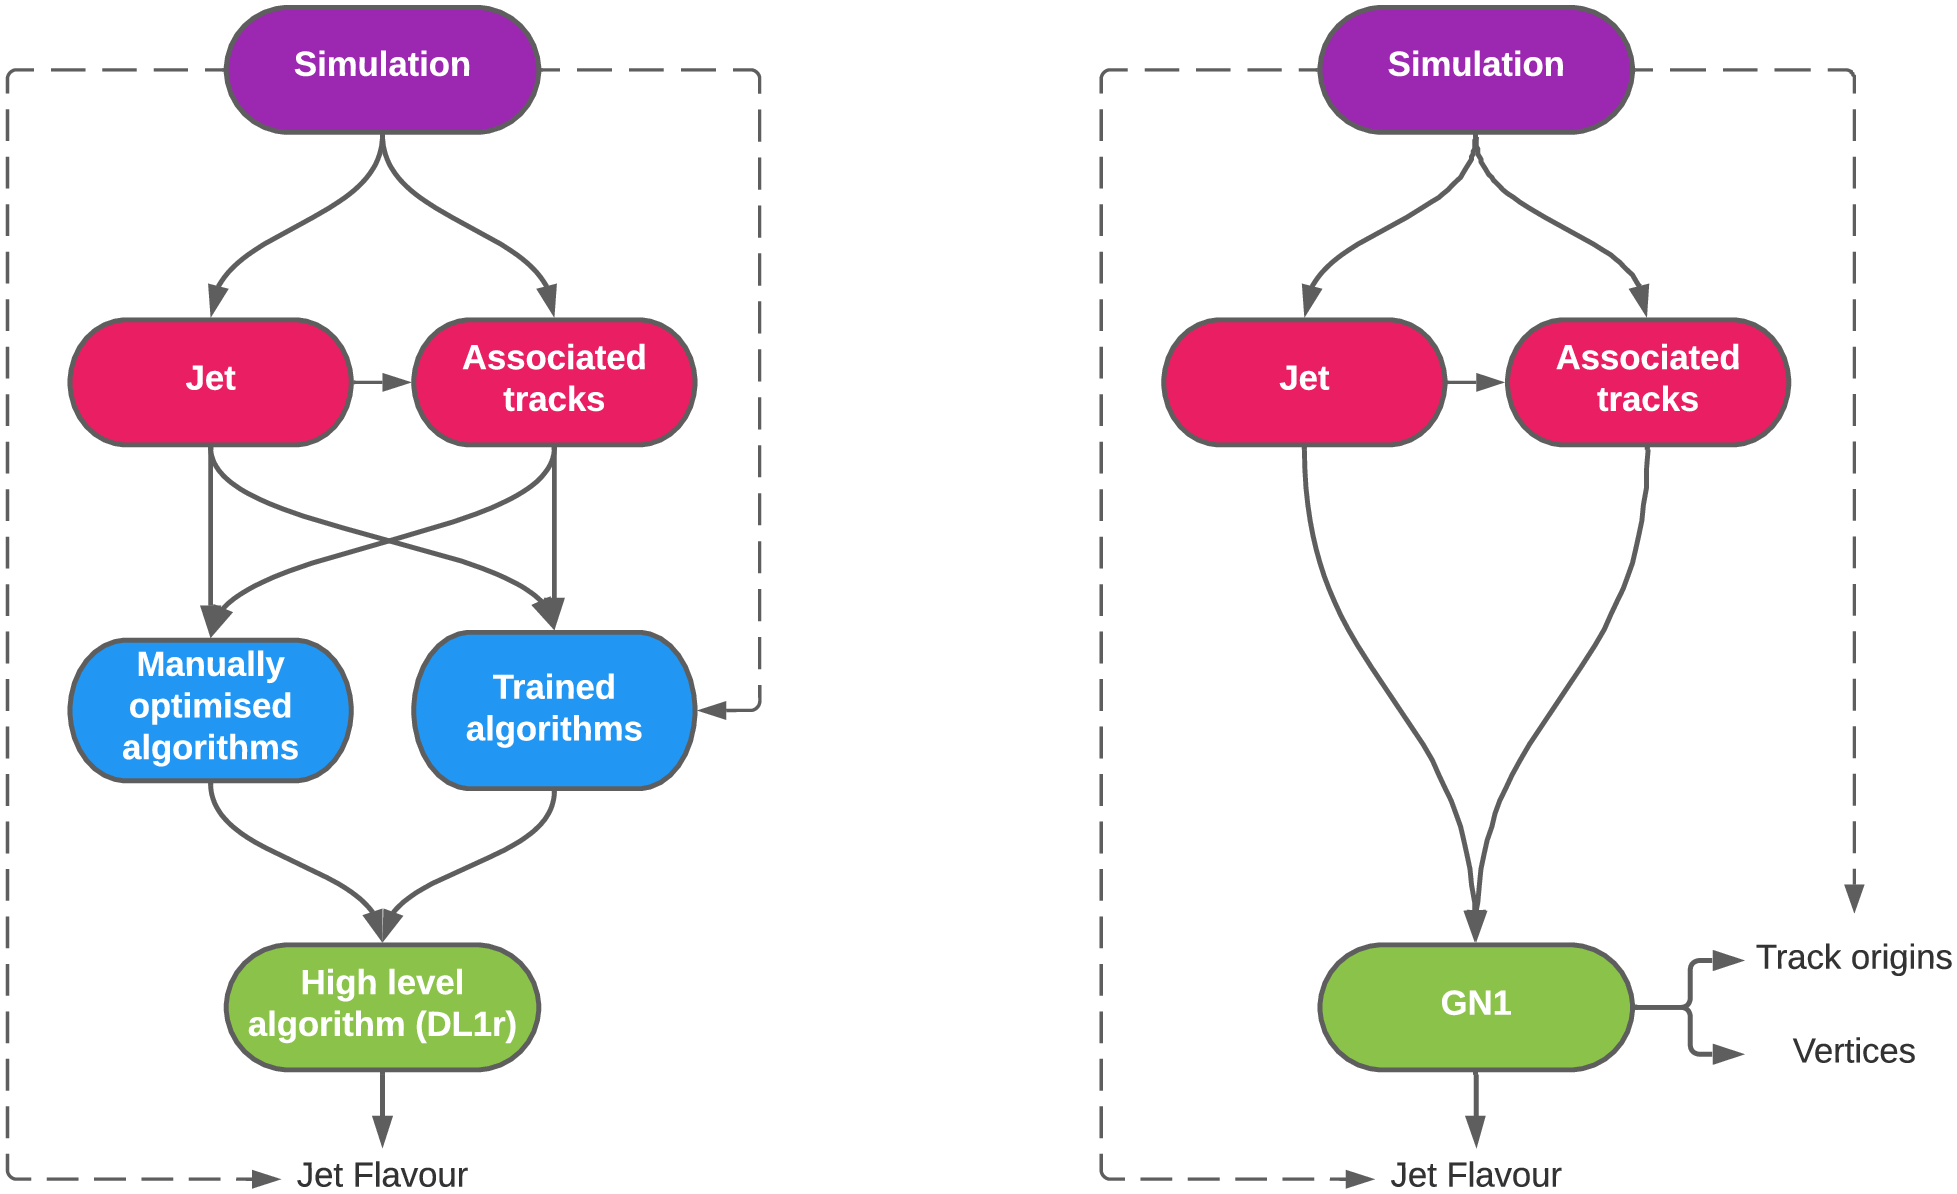
\includegraphics[width=0.9\textwidth]{Images/FTAG/GN/Intro/schematics_difference.png}
  \caption{Comparison of the tagging scheme between the DL1 family (left) and the GN family (right) \cite{ATL-PHYS-PUB-2022-027}. Solid lines represent reconstructed information while dashed lines represent truth information only accessible from the simulations.} 
  \label{fig:ftagArchi}
\end{figure}

\paragraph{}\gls{gn1} uses the information associated with charged tracks in a jet to directly output the flavour-tag probabilities, which are then combined into analogous discriminants to Equations \ref{bdisc} and \ref{cdisc}. This constitutes the primary goal of the network. Alongside predicting the flavour of the jet, auxiliary objectives are also optimised to aid and guide the training. This so-called \textit{multitasking} framework is a common way to distil expert knowledge into the design of an \gls{ml} method, focusing the attention of the network on multiple metrics. In this case, two side tasks are passed along for the physical insights they highlight.
\begin{enumerate}
\item \textit{Track origin prediction}: a classification task aiming to assign a physical process from which the track arises, as per the prescriptions detailed in Table~\ref{tab:gnTrackOrigin}. The flavour of a jet is strongly correlated to the origin of the tracks. This task brings the attention of the network to this important information as a form of supervised attention \cite{hwang2021selfsupervised}.
\item \textit{Vertex prediction}: a classification task predicting whether two tracks come from the same vertex. The decays of $b$- and $c$-hadrons include secondary and tertiary vertices inside a jet. Highlighting the compatibility of two tracks to share a vertex allows the model to infer the presence of such vertices. On the truth side, vertices separated by a distance < 0.1 mm are merged, and tracks labelled as Pile-up or Fake are forced to not have any shared vertex.
\end{enumerate}
These complementary objectives use truth information from the simulation and cannot therefore be predicted at inference time on real data. They improve performance during the training by providing useful information on the content of the jets. A modified approach in which a model is pre-trained on the auxiliary objectives and then fine-tuned on the primary objective is not observed to lead to a gain in performance, hence the objectives are optimised simultaneously. \\

\begin{table}[h]
  \begin{center}
      \begin{tabular}{ll} 
      	 \hline \hline
          Truth Origin & Description \\ \hline
          Pile-up           & From a $pp$ collision other than the primary interaction   \\
          Fake             & Created from the hits of multiple particles  \\
          Primary          & Does not originate from any secondary decay  \\
          fromB            & From the decay of a $b$-hadron  \\
          fromBC           & From a $c$-hadron decay, which itself is from the decay of a $b$-hadron   \\
          fromC            & From the decay of a $c$-hadron \\
          OtherSecondary   & From other secondary interactions and decays  \\ \hline \hline
      \end{tabular}
    \caption{Truth origins used to label the physics process leading to the produced tracks \cite{ATL-PHYS-PUB-2022-027}. Charged particles and tracks are matched using the truth matching probability \cite{ATLAS-tracks-algo}, and a value below 0.5 is taken to imply the reconstructed track parameters are mismeasured.}
    \label{tab:gnTrackOrigin}
  \end{center}
\end{table}

\begin{table}[h]
  \begin{center}
      \begin{tabular}{rl} 
      	 \hline \hline
          \multicolumn{2}{c}{Jet Inputs}\\ \hline
          $p_t$   & Jet transverse momentum \\ 
          $\eta$  & Signed jet pseudorapidity \\ \hline \\
          \multicolumn{2}{c}{Track Inputs}\\ \hline
          $q/p$             & Track charge divided by momentum (curvature)  \\
          $d\eta$           & Pseudorapidity of the track, relative to the jet $\eta$ \\
          $d\phi$           & Azimuthal angle of the track, relative to the jet $\phi$ \\
          $d_0$             & Closest distance from the track to the PV in the longitudinal plane  \\
          $z_0 \sin\theta$  & Closest distance from the track to the PV in the transverse plane  \\
          $\sigma(q/p)$     & Uncertainty on $q/p$ \\
          $\sigma(\theta)$  & Uncertainty on track polar angle $\theta$ \\
          $\sigma(\phi)$    & Uncertainty on track azimuthal angle $\phi$ \\
          $\sigma(d_0)$     & Lifetime signed transverse \gls{ip} significance \\
          $\sigma(z_0)$     & Lifetime signed longitudinal \gls{ip} significance \\
          nPixHits          & Number of Pixel hits \\
          nSCTHits          & Number of \gls{sct} hits \\
          nIBLHits          & Number of \gls{ibl} hits \\
          nBLHits           & Number of B-layer hits \\
          nIBLShared        & Number of shared \gls{ibl} hits \\
          nIBLSplit         & Number of split \gls{ibl} hits \\
          nPixShared        & Number of shared Pixel hits \\
          nPixSplit         & Number of split Pixel hits \\
          nSCTShared        & Number of shared \gls{sct} hits \\
          %nPixHoles         & Number of Pixel holes \\
          nSCTHoles         & Number of \gls{sct} holes \\ \hline \hline
      \end{tabular}
    \caption{Input features of the GN family of models \cite{ATL-PHYS-PUB-2022-027}.}
    \label{tab:gnInputVariables}
  \end{center}
\end{table}

Being built around a graph computation, the \gls{gn1} and \gls{gn2} networks are directly adapted to work with a variable number of unordered inputs. The input is composed of 21 tracks with track features listed in Table~\ref{tab:gnInputVariables}. Each track is further enriched with 2 jet-level features: the jet transverse momentum $p_T$ and pseudorapidity $\eta$. Tracks are selected from a set of requirements slightly modified from those used for \gls{dips}: $\geq$ 8 hits in the silicon layers with $<$ 2 shared hits, $<$ 3 holes in the silicon layers, $<$ 2 holes in the pixel detector, and tracks must have $p_T > 0.5$ GeV, $|d_0| < 3.5$ mm, and $|z_0 \sin\theta| < 5$ mm. A hole is a missing hit that was expected on a layer between two recorded hits of the same track. At most the first 40 tracks associated with a jet as ranked by transverse \gls{ip} significance $s_{d_0}$ are selected for processing. The input feature list includes missing information from the track and shared hits to specifically target high $p_T$ jets, where tracks are more collimated and their separation can be unresolvable with the deployed detector technology. The \gls{gn1} and \gls{gn2} models share the properties presented so far. They however differ in their architecture, which is explored in further detail in the next two sections.

\subsection{GN1: Graph Attention Network for Flavour Tagging}\label{chap-GN1}
The architecture of \gls{gn1}, described in Figure~\ref{fig:gnnArchitecture}, relies on a modified graph attention network \cite{brody2022how} specifically designed for graph learning on sets, the so-called \textit{Set2Graph} \cite{serviansky2020set2graph}. The design of the network architecture was subject to coarse hyperparameter optimisation. The first step takes all tracks, each represented by a vector of features composed of the 21 track features plus the two jet features, and embeds each of these track vectors into a latent space of dimension 64 with a feed-forward network of three hidden layers with 64 neurons. This is similar to the track neural network $\Phi$ of the \gls{dips} model. \\

\begin{figure}[h!]
  \center
  \hspace{-1.6cm}
  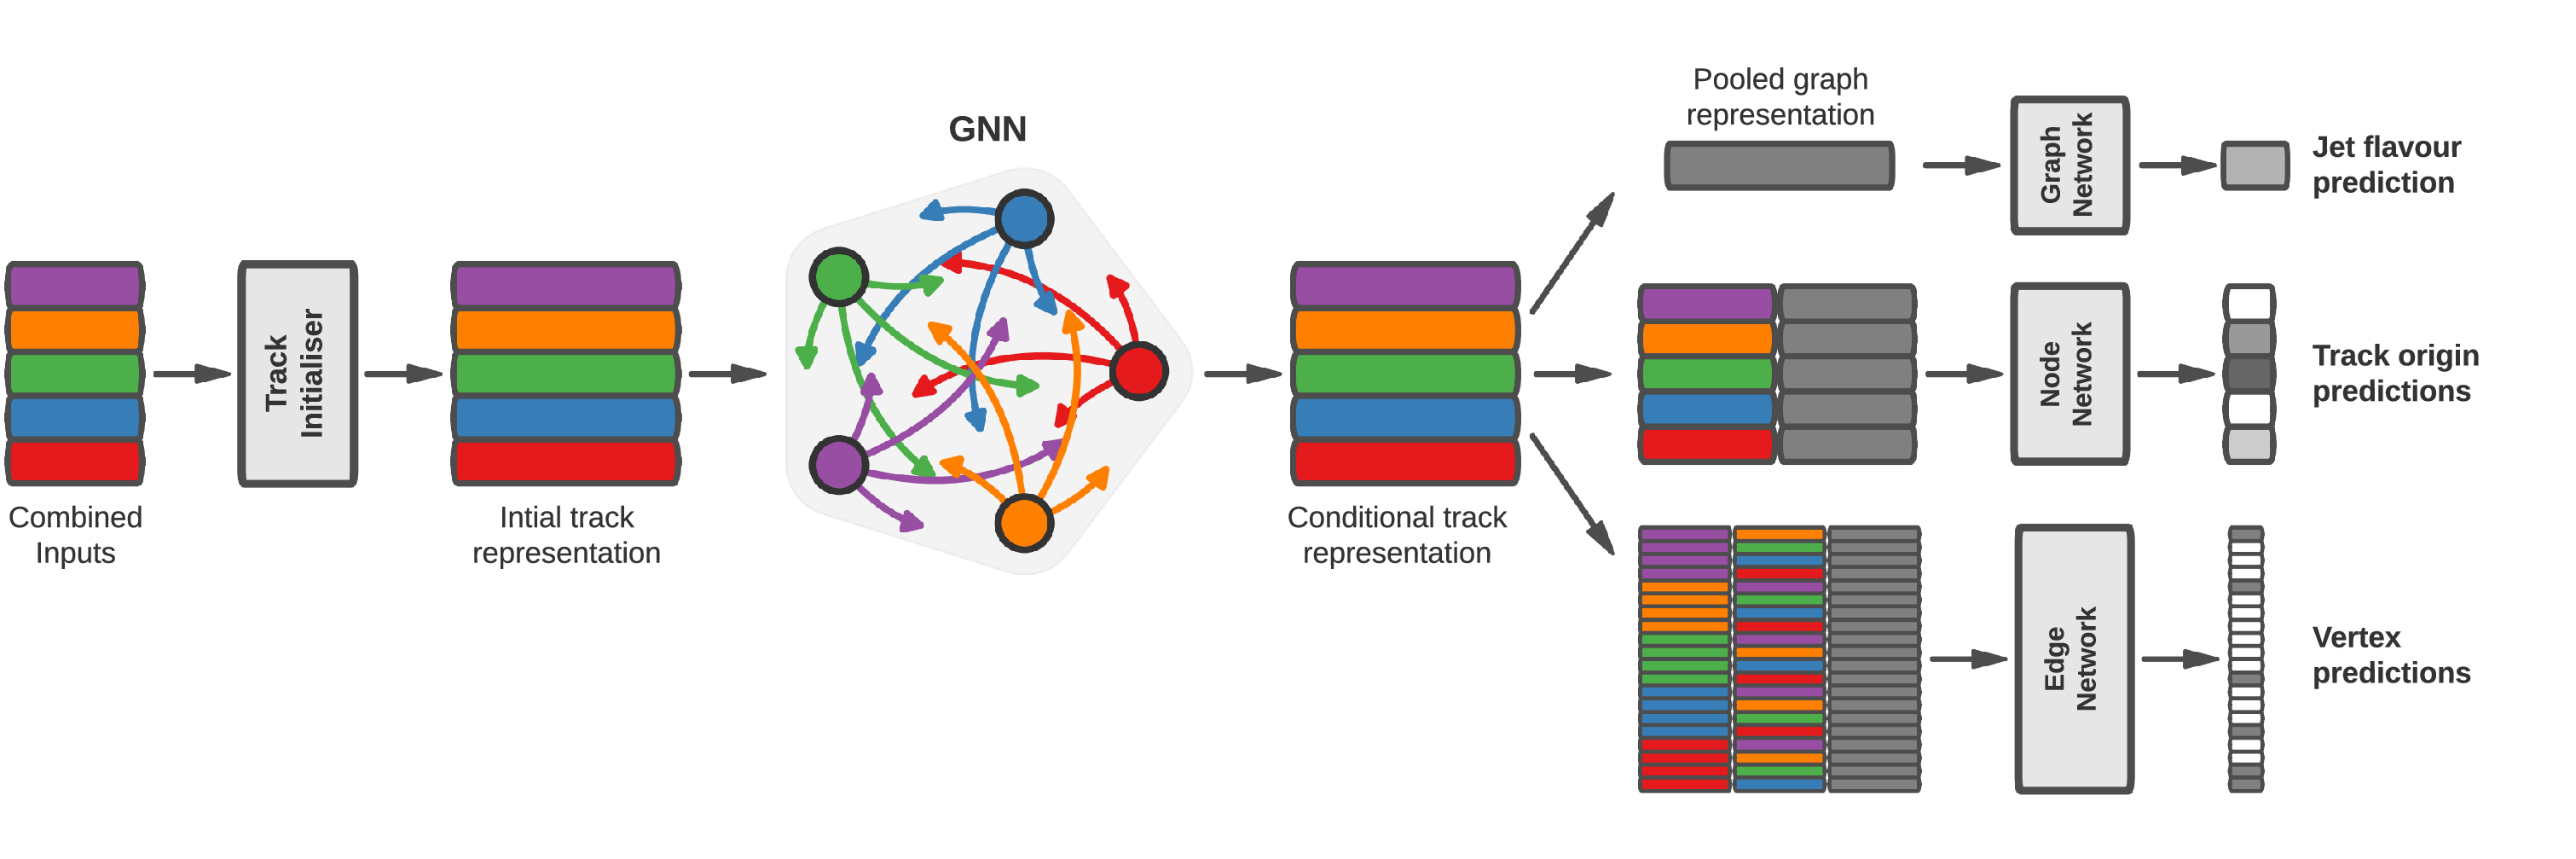
\includegraphics[width=1.1\textwidth]{Images/FTAG/GN/Intro/gnn_architecture.png}
  \caption{The architecture of the GN1 network \cite{ATL-PHYS-PUB-2022-027}. The combined input is made of the set of tracks, each of which is given a copy of the two jet variables in addition to the track features, as described in Table~\ref{tab:gnInputVariables}. After a first embedding taking the input to an enriched latent representation, a fully connected graph is defined with the embedded tracks as nodes. The output of the graph is a conditional track representation used by the three training objectives.} 
  \label{fig:gnnArchitecture}
\end{figure}

A fully-connected graph is built with the embedded track representations as nodes. For this section, there is one node per track labelled $h_i$ and represented by a feature vector of dimension 64. The graph network updates the defined graph $G(\mathcal{N})$ into a graph $G'(\mathcal{N}')$, with $\mathcal{N}$ and $\mathcal{N}'$ the set of nodes, by aggregating the features of each vertex $h_i$ and neighbouring nodes $\mathcal{N}_i$ to $h_i$ using the operation of Ref. \cite{brody2022how}. In the present case, the graph is fully connected, hence $\mathcal{N}_i = \mathcal{N}$. The following 4 steps are applied during a single graph update \cite{ATL-PHYS-PUB-2022-027}:
\begin{enumerate}
  \item Each node feature vector is passed through a fully connected layer $W$ producing an updated representation $W\,h_i$ of size 64.
  \item Pairwise scalar edge scores are computed for each pair of nodes $i, j \in \mathcal{N}$ by 
  \begin{equation}
    e\left(h_i, h_j\right) = V^T \theta\left([Wh_i, Wh_j]\right),
  \end{equation}
  where $V$ is a second feed-forward layer of size 128, $\theta$ is the \gls{relu} activation function, and $[,]$ stands for the concatenation operation of two tensors. 
  \item Attention weights are derived from the pairwise edge scores, using a softmax over all $j$ per node $h_i$:
  \begin{equation}
    a_{i,j} = \textrm{softmax}_j\left(e(h_i, h_j)\right).
  \end{equation}
  \item The final step is to aggregate the information to update each node $h_i \rightarrow h'_i$ by computing the attention-weighted sum over all node representations $\forall j \in \mathcal{N}$: 
  \begin{equation}
    h'_i = \sum_{j} a_{i,j} \,.\, W h_j,
  \end{equation} 
\end{enumerate}

For \gls{gn1}, applying 2 attention heads with 3 successive graph network layers is found to deliver optimal performance without any overtraining observed. The outputs of the graph network are \textit{conditional track representations}, updating every track representation with information from other tracks. The ordering of the conditional tracks is kept similar to that of the original set to match processed tracks to their truth information. Furthermore, a global representation is derived by combining the conditional track representation with a pooling operation using learnable attention weights. These rich conditional and global representations can now be passed as inputs to three distinct feed-forward neural networks leading to the different objectives \cite{ATL-PHYS-PUB-2022-027}:
\begin{enumerate}
  \item \textit{Jet flavour prediction}: performed by a graph classification network that is only fed the global representation. The primary objective of predicting the jet flavour is done by this network, composed of 4 hidden layers with 128, 64, 32, and 16 neurons respectively, finishing on an output of size 3 with a softmax activation for $b$-, $c$-, and light-jet probabilities.
  \item \textit{Track origin prediction}: performed by a node classifier processing each conditional track representation with the global representation. This network is built with three layers of reducing width 128, 64, and 32, to finish on the output layers of size 7 with a softmax activation, matching to the 7 classes corresponding to the different truth origins considered in Table~\ref{tab:gnTrackOrigin}.
  \item \textit{Vertex prediction}: performed by a node-pairs binary classifier that receives every possible combination of conditional track representations as well as the global representation. This network is made of 3 layers of size 128, 64, and 32 for a final output of size 1 with a sigmoid activation, stating whether the pair of tracks have a common vertex or not. 
\end{enumerate}

The architecture of \gls{gn1} is somewhat akin to an enhanced version of \gls{dips}, with the track initialiser and graph classifiers corresponding to $\Phi$ and $F$. Added elements are the powerful \gls{gnn} layers, the conditional representation pooling layer with attention, and the auxiliary objectives. \gls{gn1} is trained by  minimising the combined loss function $\mathcal{L}_{\textrm{total}}$ defined as 
\begin{equation}\label{eq:totalobjgn}
  \mathcal{L}_{\textrm{total}} = \mathcal{L}_{\textrm{flavour}} + \alpha \, \mathcal{L}_{\textrm{track}} + \beta \, \mathcal{L}_{\textrm{vertex}}.
\end{equation}
$\mathcal{L}_{\textrm{flavour}}$ is the categorical cross-entropy loss, as defined in Equation \ref{eq:statEntropy}, over the different jet flavours to output the per-flavour probabilities. $\mathcal{L}_{\textrm{track}}$ is the categorical cross-entropy loss for the track origin prediction averaged over all tracks in a batch. Due to intrinsic differences in the relative frequency of track origins, the contribution of each origin is weighted by its inverse frequency of occurrence. Finally, $\mathcal{L}_{\textrm{vertex}}$ is the binary cross-entropy of the track-pair compatibility averaged over all track-pairs in a batch. The importance of matching tracks from $b$- and $c$-hadrons is artificially increased by doubling the weights of their track-pairs. In Equation \ref{eq:totalobjgn}, special weights are applied to combine the different tasks that are represented by distinct values, reflecting their specific loss functions and difficulties. Weights of $\alpha = 0.5$ and $\beta = 1.5$ \cite{ATL-PHYS-PUB-2022-027} lead the auxiliary objectives to converge to similar values, giving the different additional terms equal weighting in $\mathcal{L}_{\textrm{total}}$. This choice of parameters also lets the primary objective $\mathcal{L}_{\textrm{flavour}}$ dominate the global loss, with small variations of $\alpha$ and $\beta$ not significantly impacting the performance. The results presented here come from Ref. \cite{ATL-PHYS-PUB-2022-027}, where a \gls{gn1} model is trained for 100 epochs with a sample of 30 million jets made of 60\% $t\bar{t}$ and 40\% $Z'$, as previously described in this chapter. The validation loss on a statistically independent sample of 500k jets is monitored, with the epoch minimising it selected for further analysis. The optimiser is based on Adam \cite{adamPaper} with a learning rate of $10^{-3}$ and a batch size of 4000 jets spread across 4 \glspl{gpu}. \\


\begin{figure}[h!]
  \centering
  \begin{subfigure}[b]{0.98\textwidth}
      \centering
      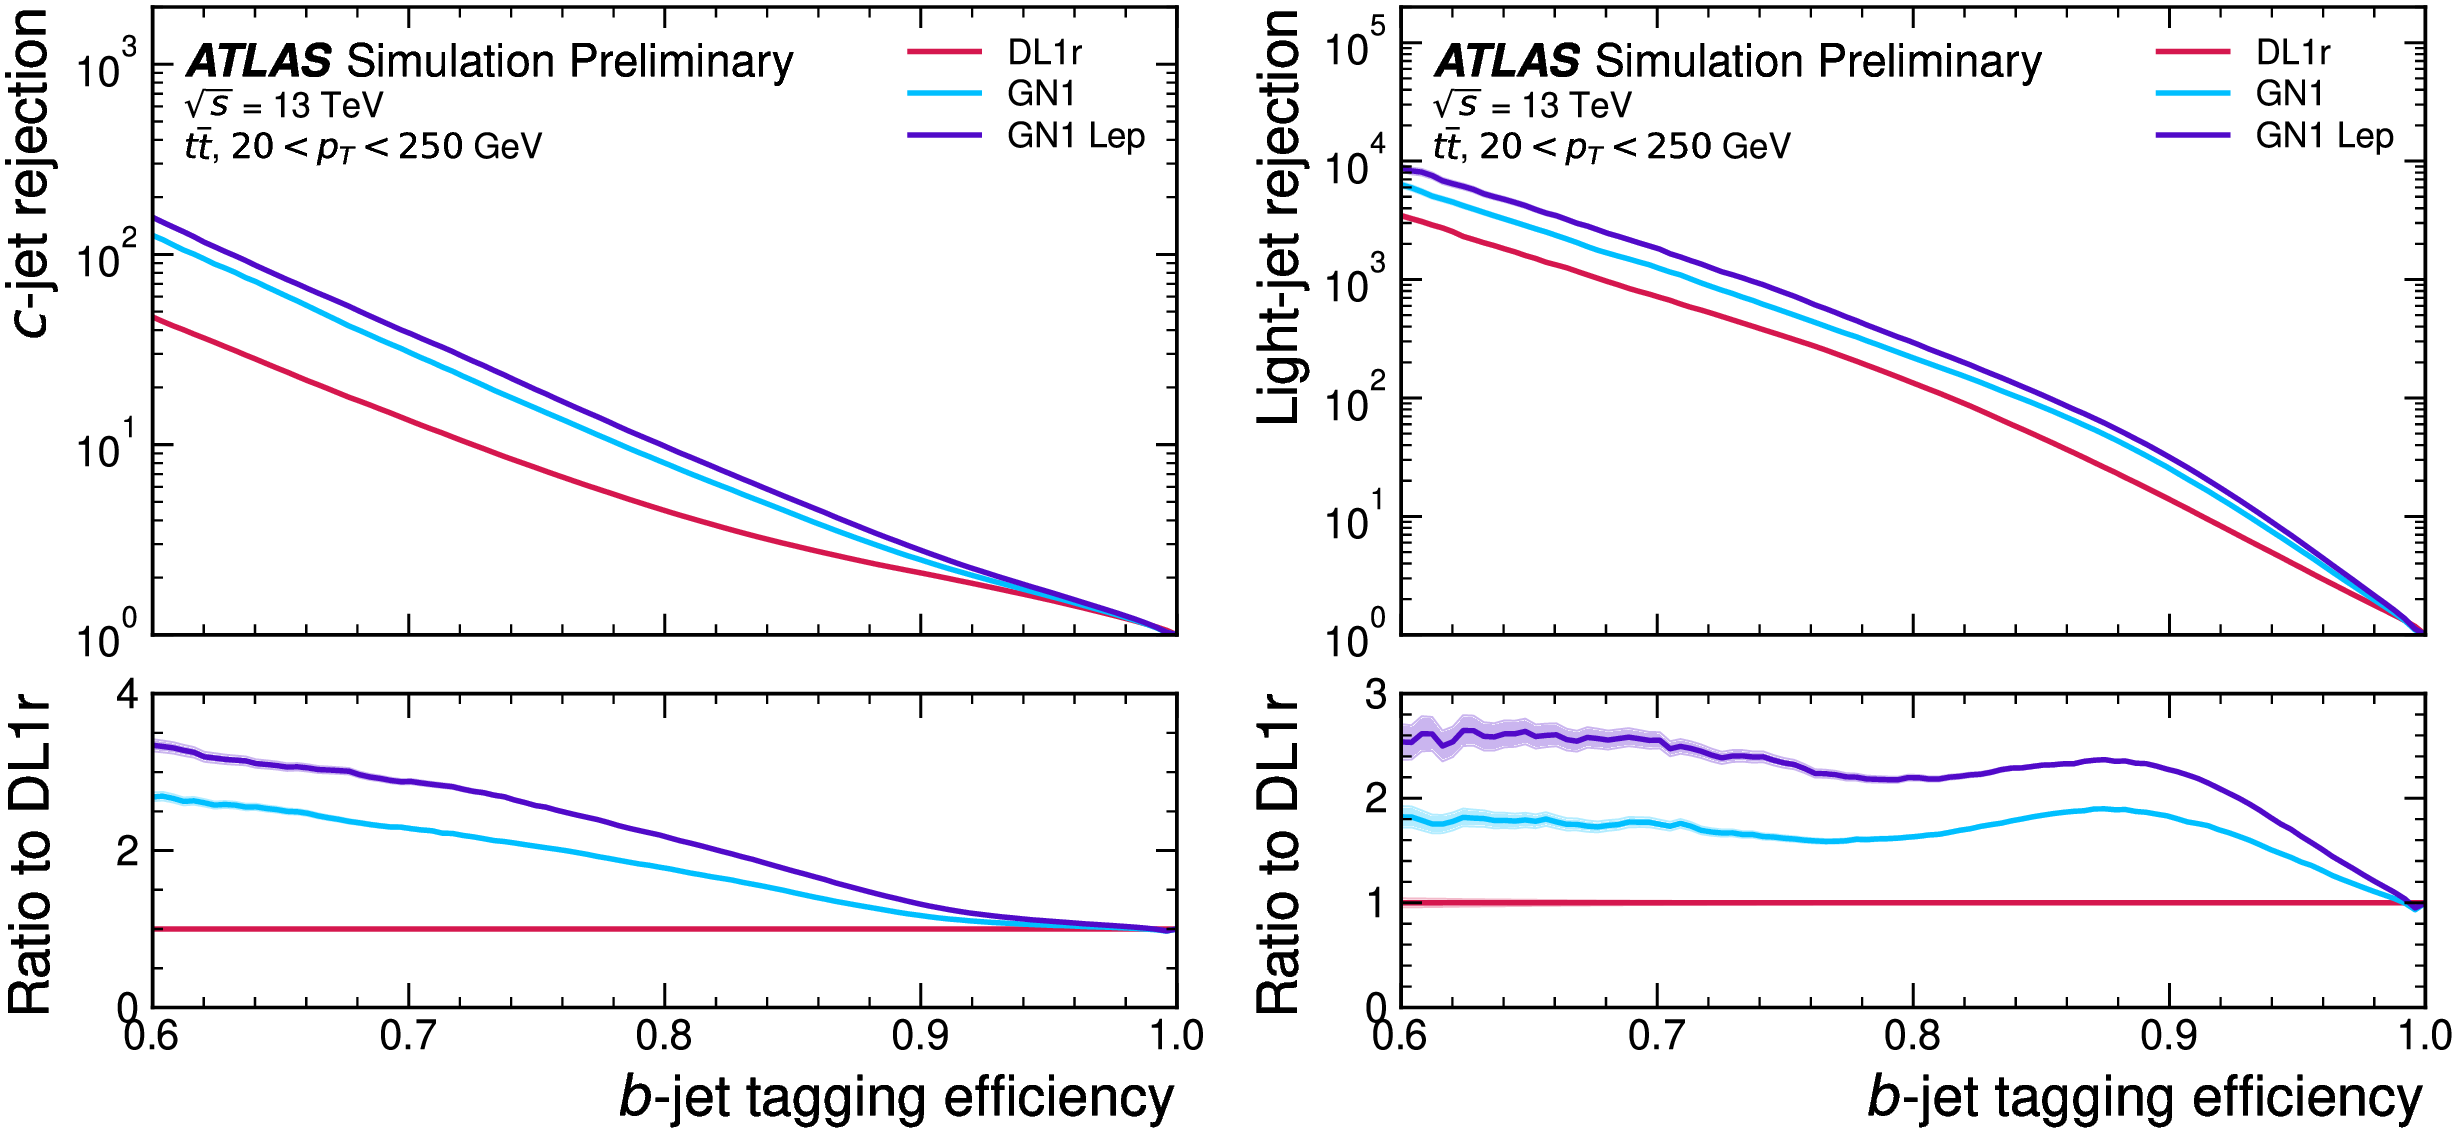
\includegraphics[width=0.98\textwidth]{Images/FTAG/GN/GN1/ROC/ttb.png}
      \caption{GN1 and DL1r performance on the $t\bar{t}$ test sample, with $20 < p_T < 250$ GeV.} 
      \label{fig:GN1ttb}
  \end{subfigure}\\
  \begin{subfigure}[b]{0.98\textwidth}
    \centering % UNreadable: increase font size
      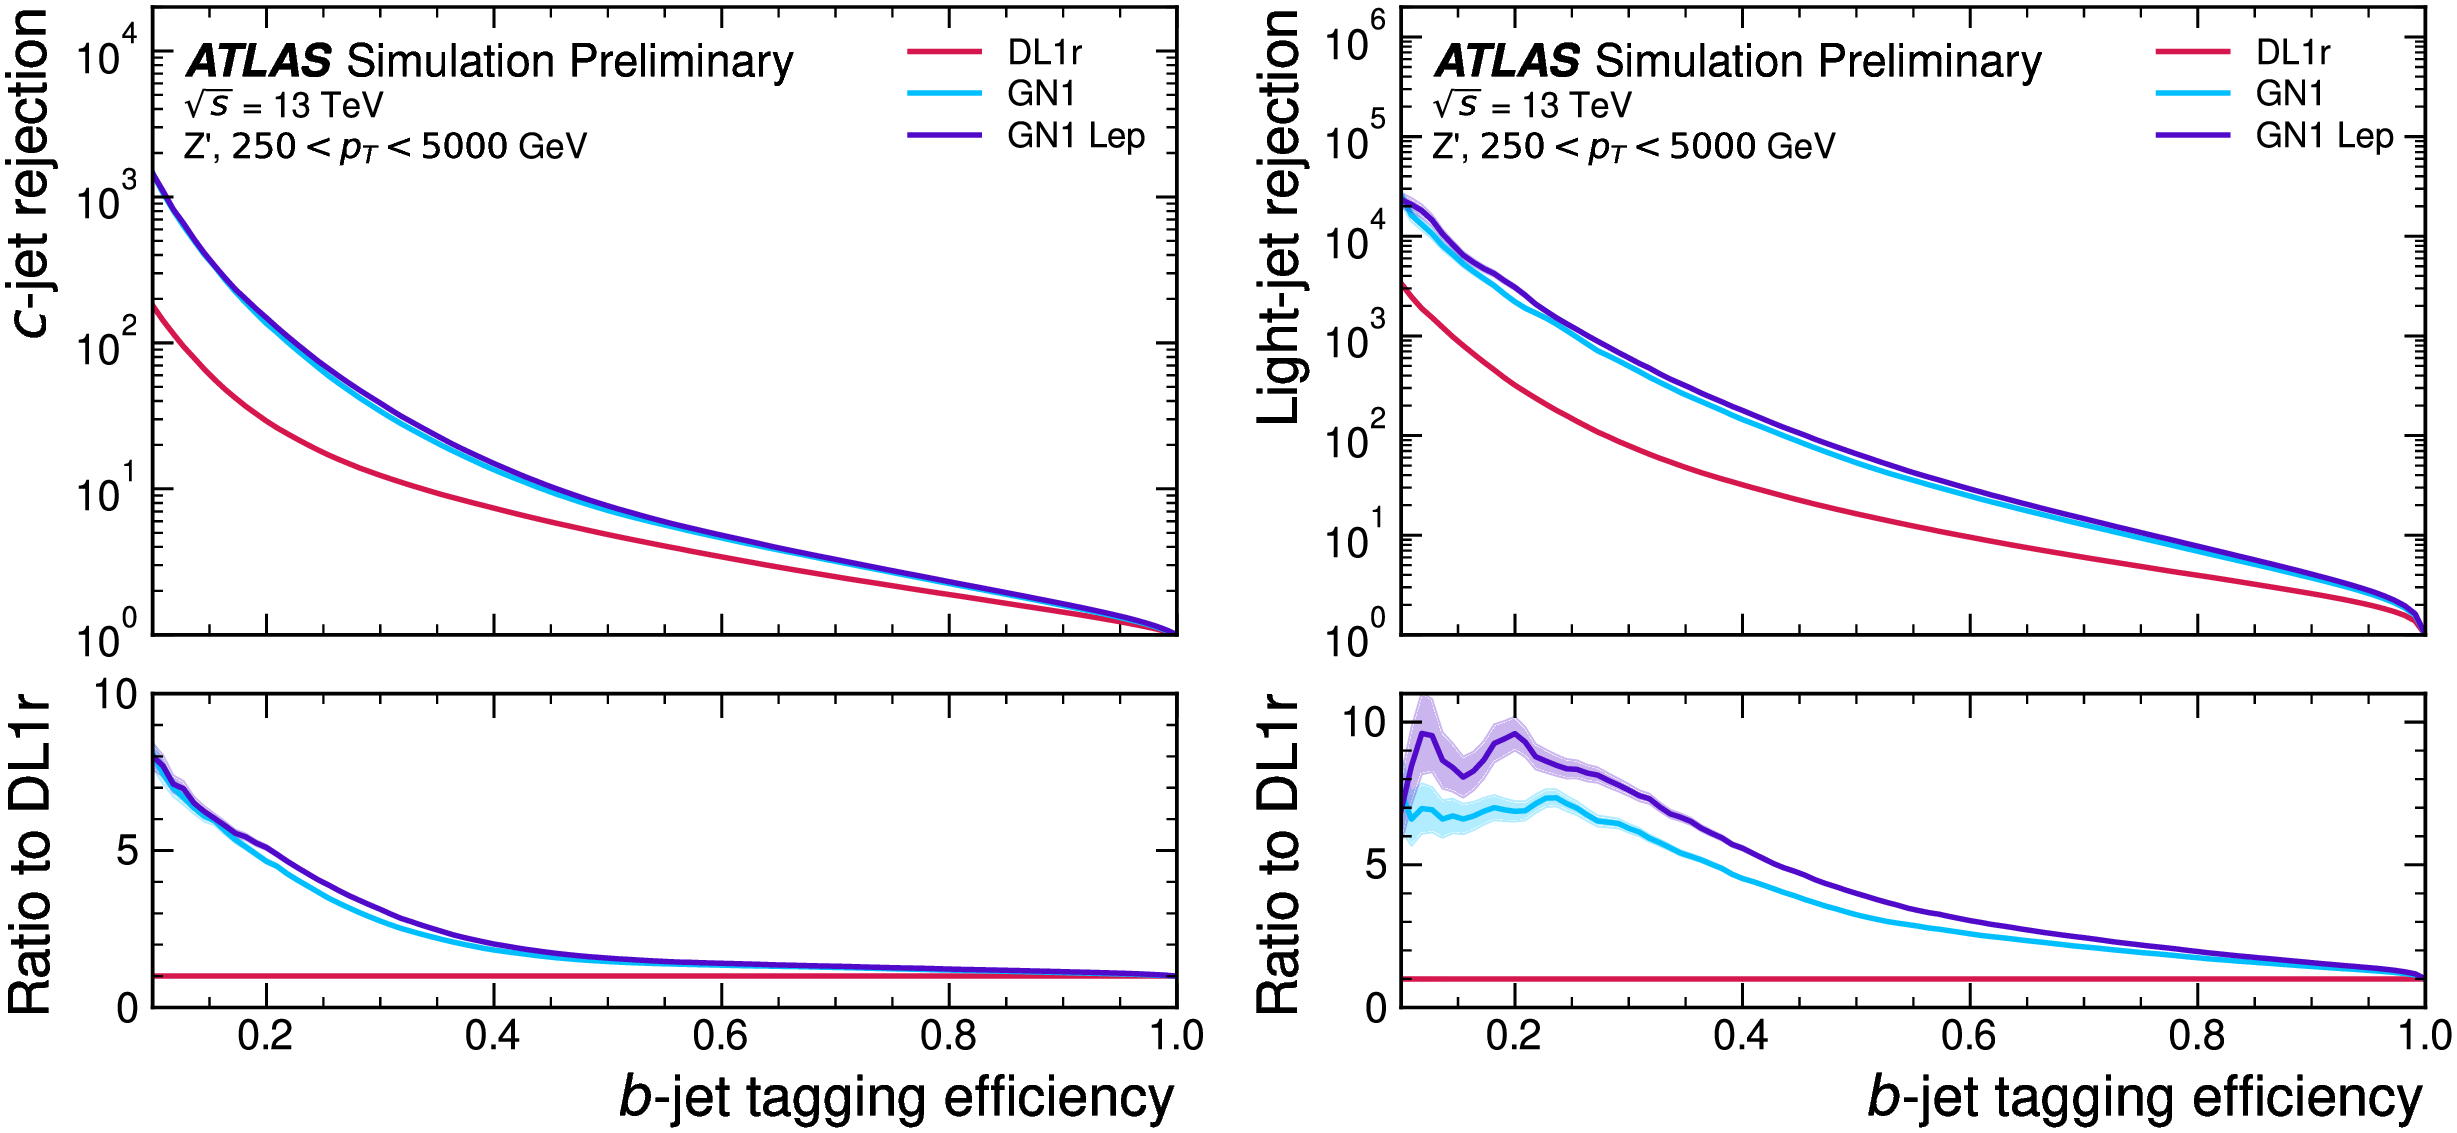
\includegraphics[width=0.98\textwidth]{Images/FTAG/GN/GN1/ROC/zpb.png}
      \caption{GN1 and DL1r performance on the $Z'$ test sample, with $250 < p_T < 5000$ GeV.} 
      \label{fig:GN1zpb}
  \end{subfigure}
  \caption{ROC curves tracing the $b$-tagging efficiency versus the $c$-jet (left) and light-jet (right) rejections for the $t\bar{t}$ (top) and $Z'$ (bottom) test samples \cite{ATL-PHYS-PUB-2022-027}. Models compared are DL1r in red, GN1 in blue, and GN1 Lep in purple. The bottom panels show the ratio to DL1r. The flavour fraction is set at $f^b_c = 0.018$ for DL1r and 0.05 for GN1 and GN1 Lep. The binomial error bands are shown as shaded regions.}
  \label{fig:GN1rocb}
\end{figure} 


The results of the training are presented in Figures \ref{fig:GN1rocb} and \ref{fig:GN1rocc} for $b$- and $c$-tagging respectively, where a \gls{dl1r} model retrained on similar inputs to the GN1 with 75 million jets is presented as reference. The \gls{roc} curves of a GN1 model with an additional track input to those of Table~\ref{tab:gnInputVariables} indicating whether a track was used in the reconstruction of an electron or a muon is also included as GN1 Lep. Most of the improvement in rejection from \gls{gn1} models is found a lower tagging efficiencies. At the typical \gls{wp} of 70\% on the low $p_T$ region defined by $t\bar{t}$, the $c$-jet (light-jet) rejection is 110\% (80\%) above that of \gls{dl1r}. As was highlighted in Figures \ref{fig:DL1dtt} and \ref{fig:DL1dz}, the performance of \gls{dl1d} is approximately 20\% to 50\% above \gls{dl1r} at the 70\% \gls{wp}, which is much lower than the observed gains made by the \gls{gn1} models. Improvements are made across the  $p_T$ spectrum, with a 180\% (500\%) increase in rejection at a 30\% \gls{wp} on $Z'$, which roughly corresponds to the efficiency obtained when applying the 70\% \gls{wp} from $t\bar{t}$ on this higher energy sample. The \gls{gn1} version with lepton information further improves the performance, to a $c$-rejection (light-rejection) of 180\% (150\%) at the 70\% \gls{wp} on $t\bar{t}$ and 180\% (600\%) on the $Z'$ at the 30\% \gls{wp}. A factor behind the observed performance improvement is the looser track selection leveraged by \gls{gn1} and the more sophisticated exploitation of the noisy set of low-level track information. The \gls{gn1} and \gls{dl1r} discriminants for $b$-tagging are presented in Figure~\ref{fig:GN1disb}. The distributions for \gls{gn1} move the $b$-jet distribution to higher values of the discriminants, indicating higher confidence in the associated predicted $p_b$. 

\newpage
\begin{figure}[h!]
  \centering
  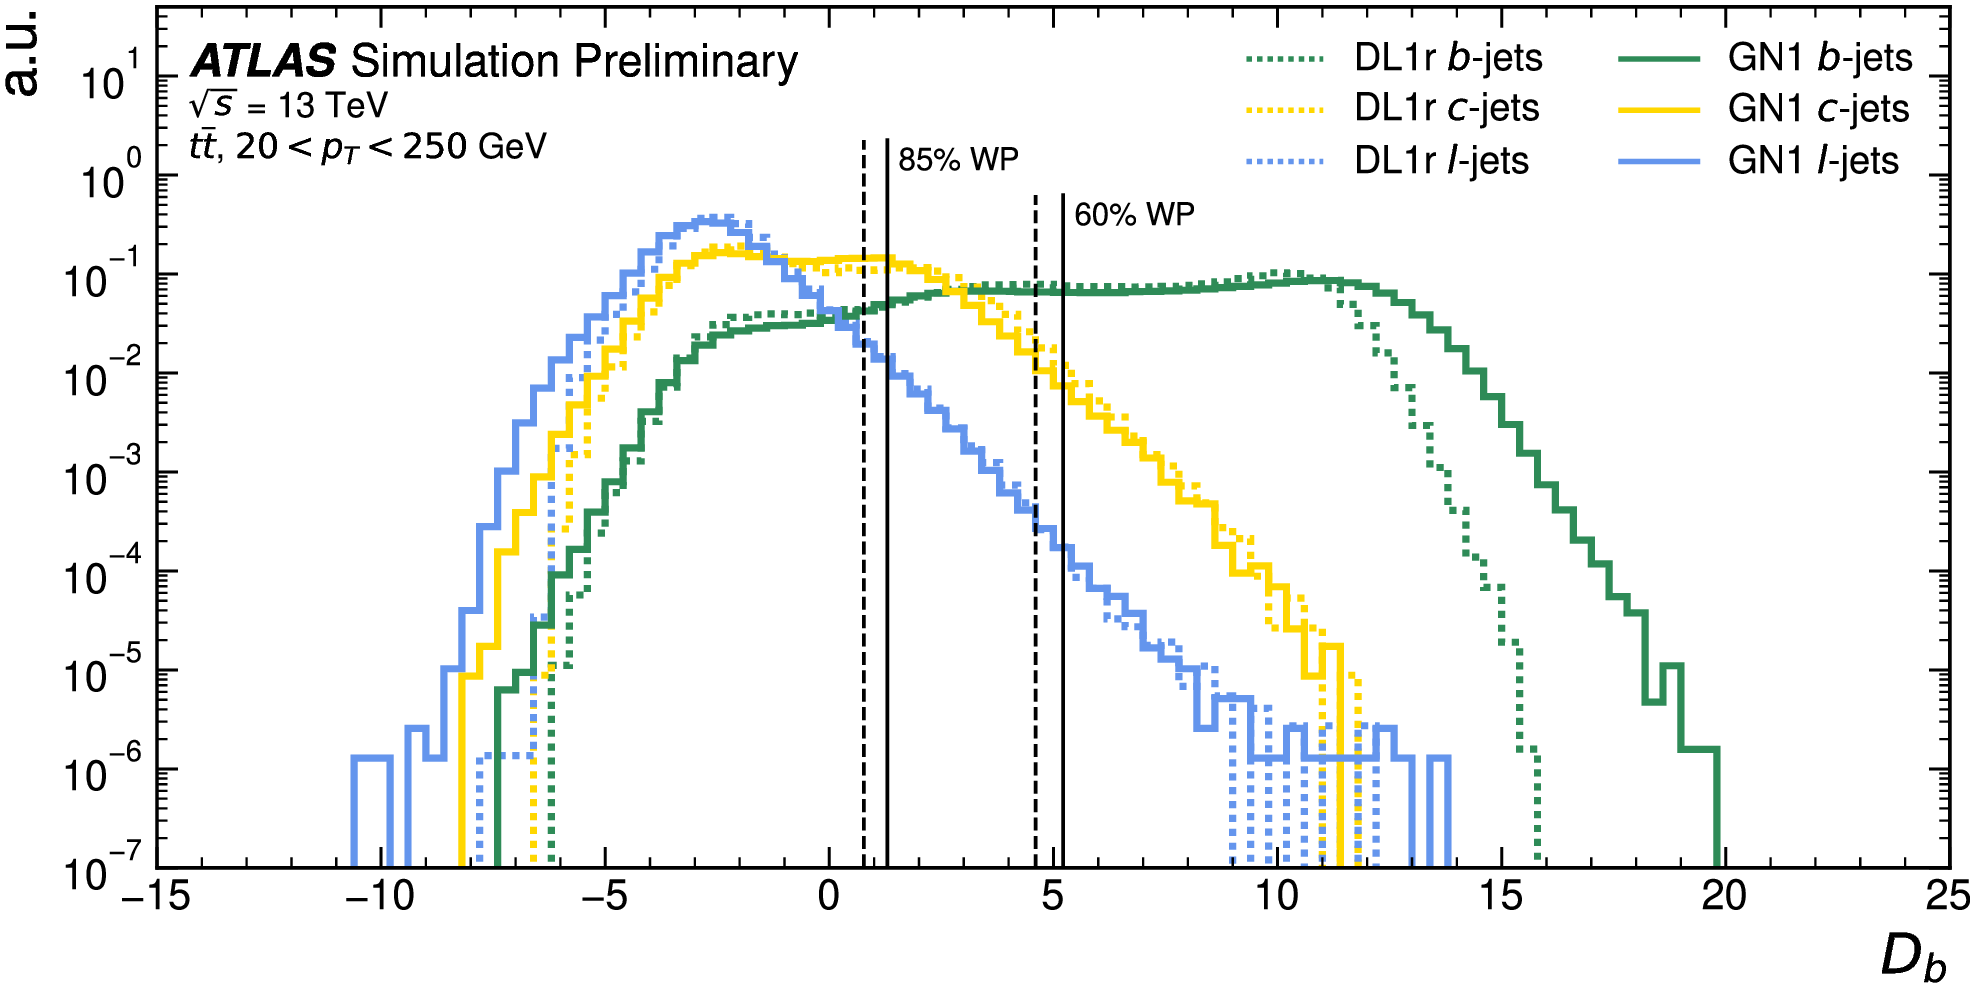
\includegraphics[width=0.8\textwidth]{Images/FTAG/GN/GN1/eff/ttb.png}
  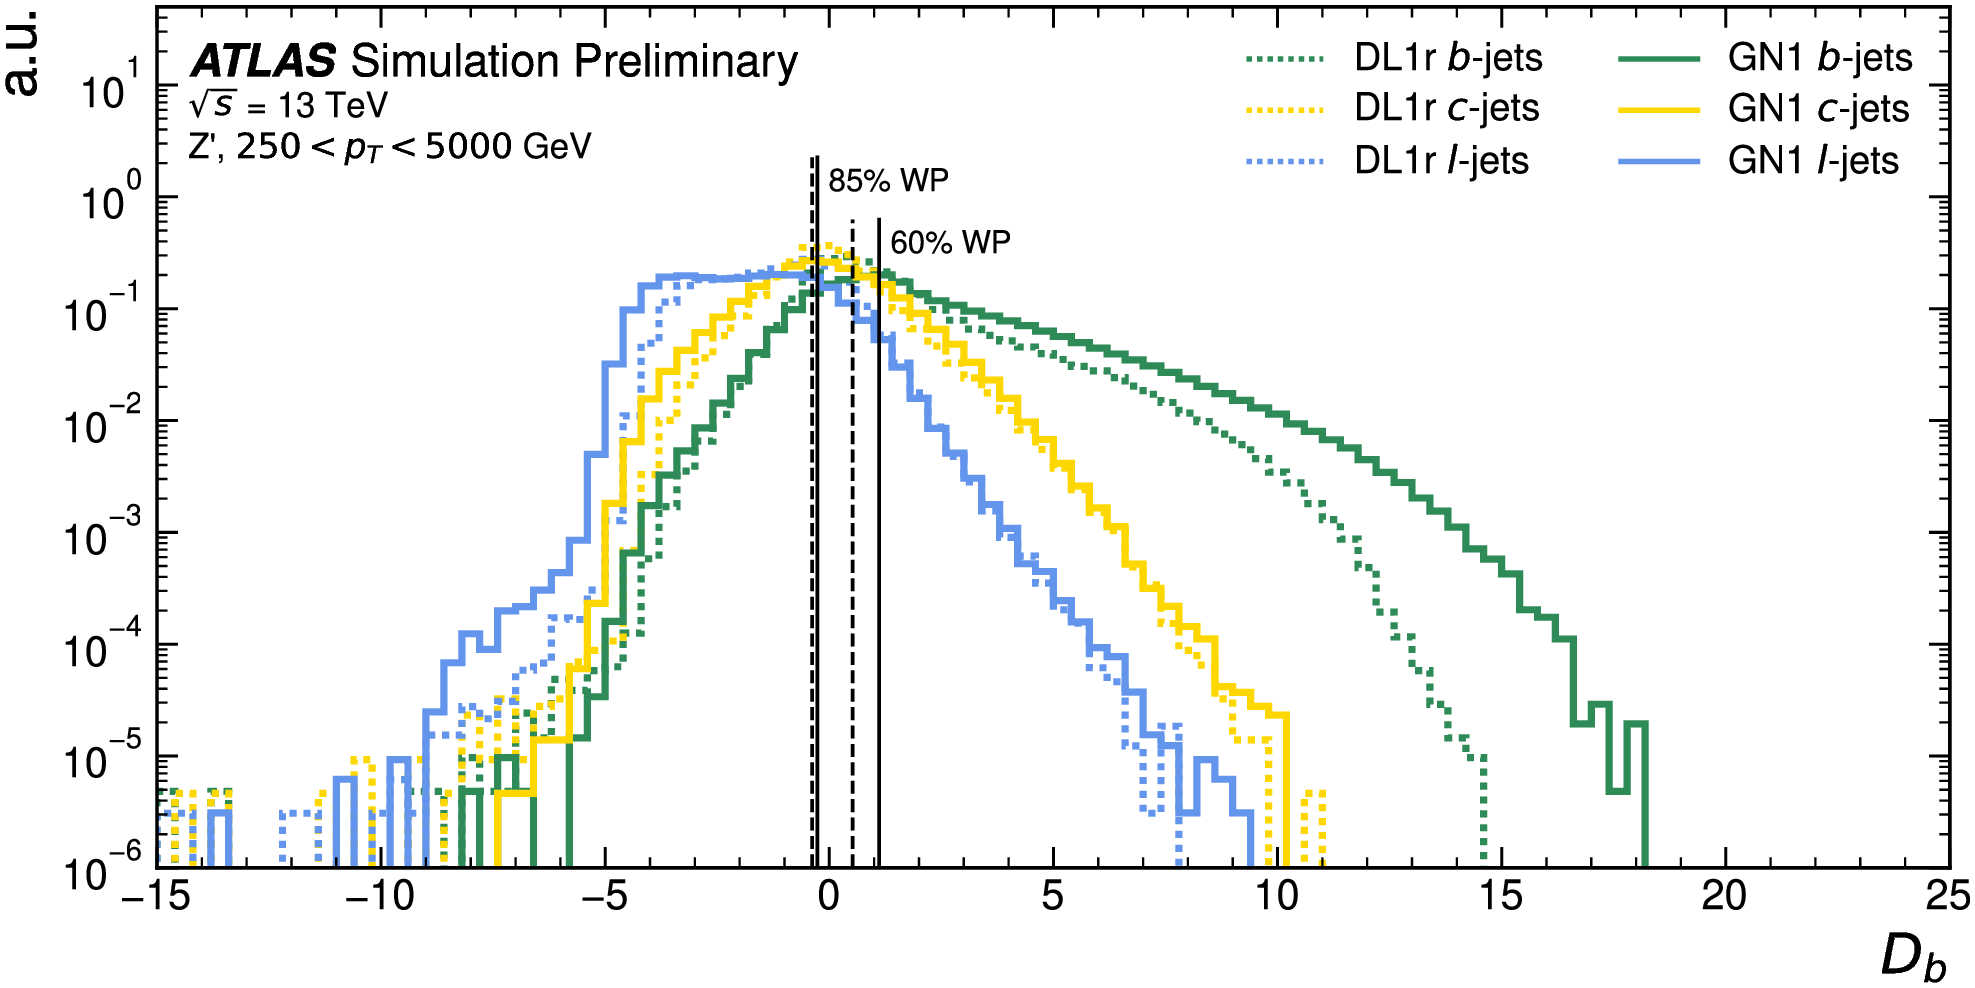
\includegraphics[width=0.8\textwidth]{Images/FTAG/GN/GN1/eff/zpb.png}
  \caption{Comparing the GN1 and DL1r $b$-tagging discriminants $D_b$ normalised distributions on the $t\bar{t}$ (top) and $Z'$ (bottom) test samples \cite{ATL-PHYS-PUB-2022-027}. Models compared are DL1r in dashed lines and GN1 in continuous lines. Flavours are indicated by a different colour: green for $b$-jets, yellow for $c$-jets, and blue for light-jets. Flavour fractions are set at $f^b_c = 0.018$ for DL1r and 0.05 for GN1.}
  \label{fig:GN1disb}
\end{figure} 

Concerning the $c$-tagging performance, the \gls{roc} curves and the discriminant distributions $D_c$ are presented in Figures \ref{fig:GN1rocc} and \ref{fig:GN1disc}. \gls{gn1} significantly outperforms \gls{dl1r} for $c$-tagging: both background rejections are doubled on the $t\bar{t}$ sampled at a $c$-tagging \gls{wp} of 25\%, with a more modest increase on the $Z'$ sample of 60\% for $b$-rejection and 100\% for light-rejection at the same $c$-tagging \gls{wp}. \\

\begin{figure}[h!]
  \centering
  \begin{subfigure}[b]{0.98\textwidth}
      \centering
      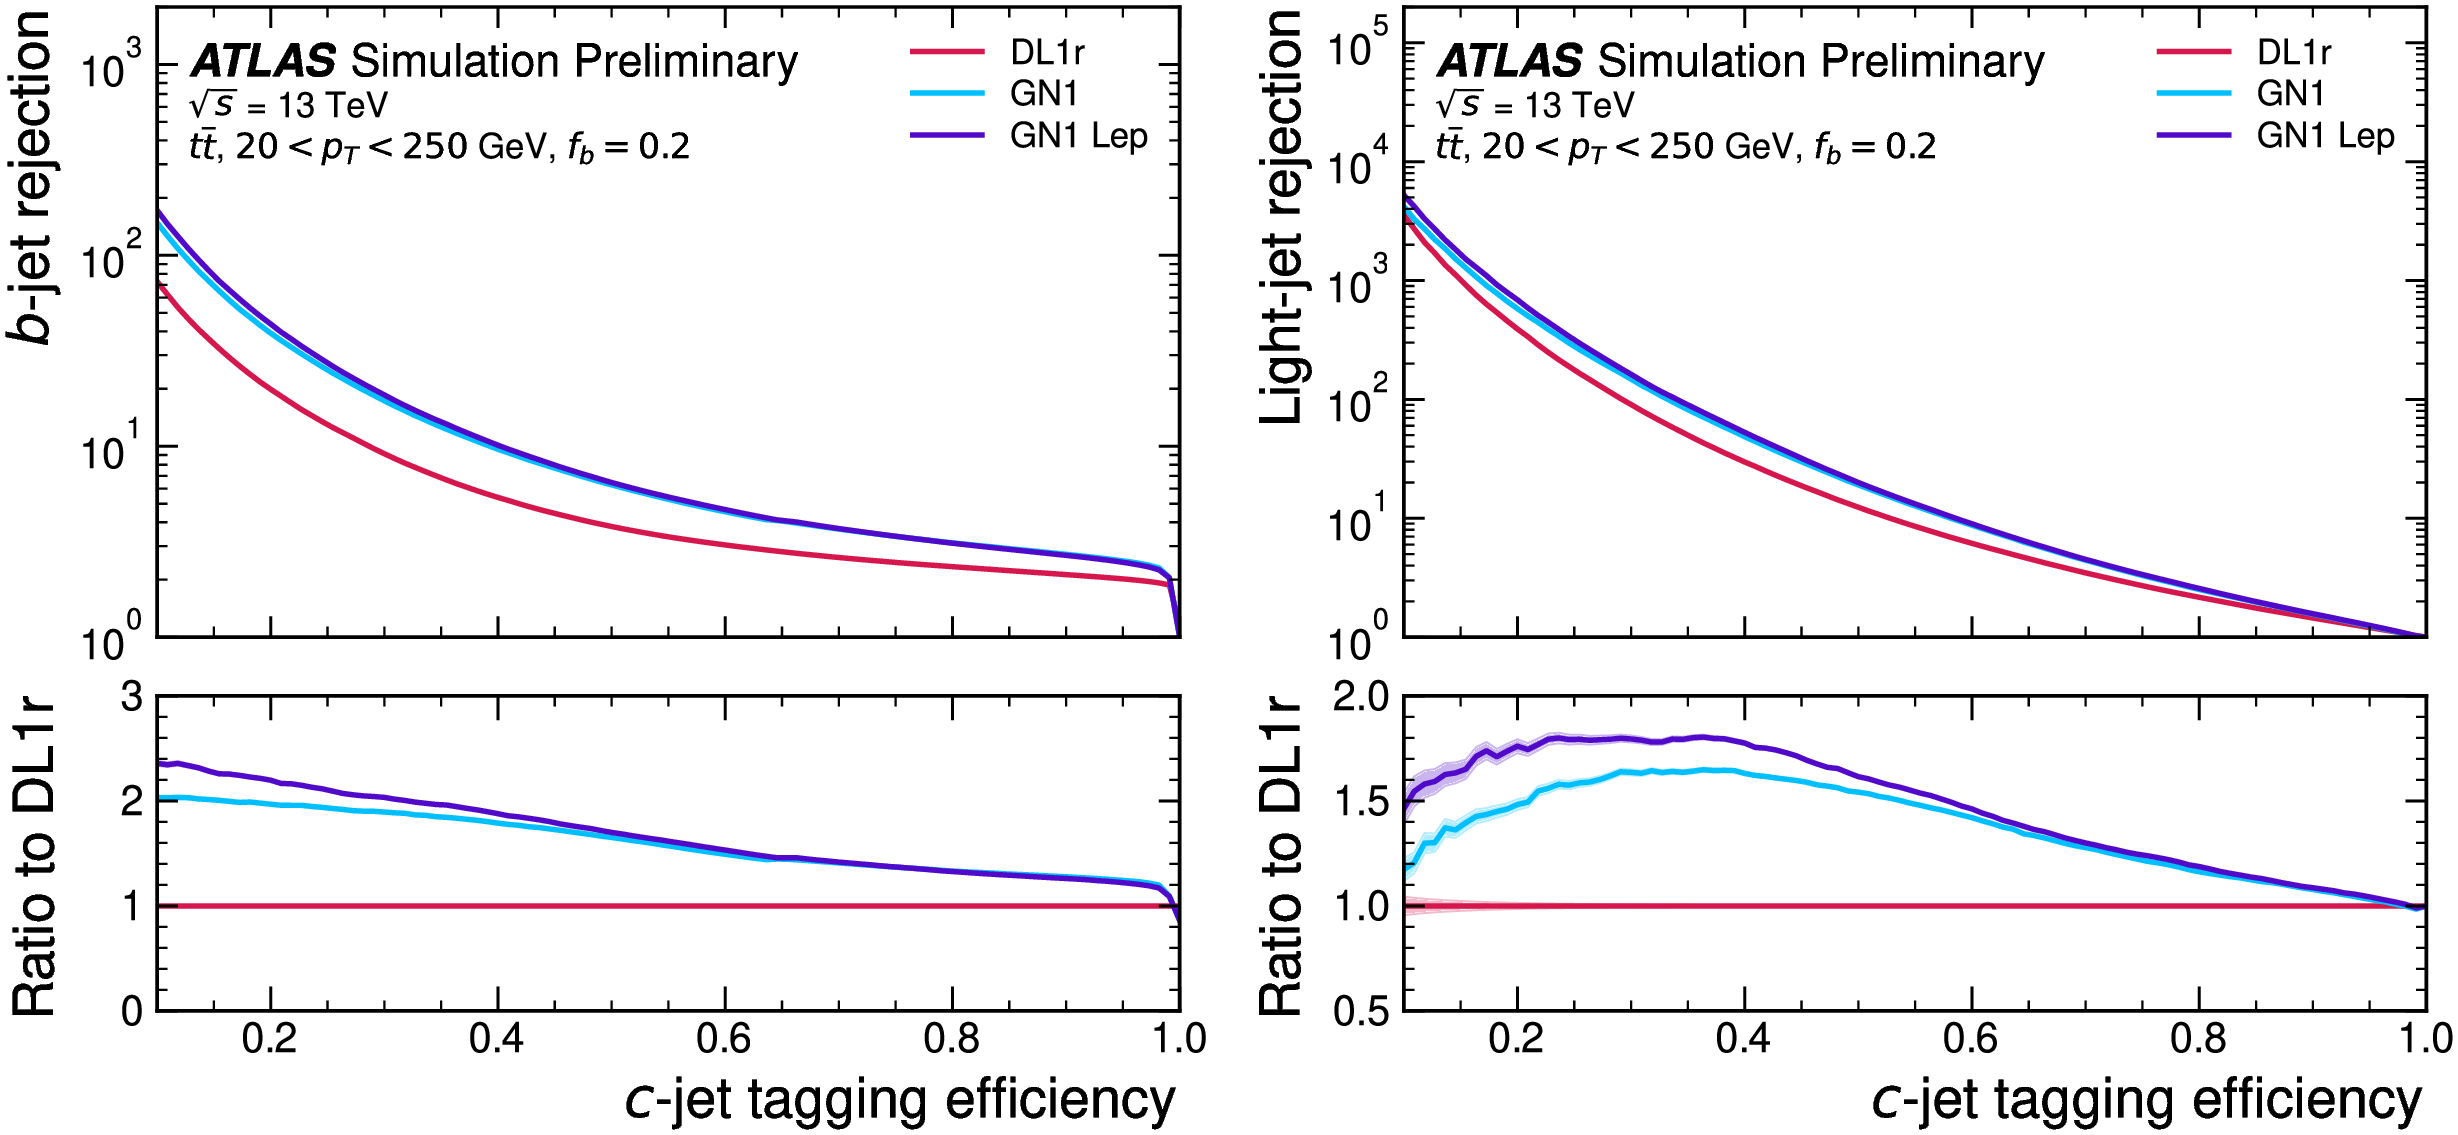
\includegraphics[width=0.98\textwidth]{Images/FTAG/GN/GN1/ROC/ttc.png}
      \caption{GN1 performance on the $t\bar{t}$ test sample, with $20 < p_T < 250$ GeV.} 
      \label{fig:GN1ttc}
  \end{subfigure}\\
  \begin{subfigure}[b]{0.98\textwidth}
    \centering
      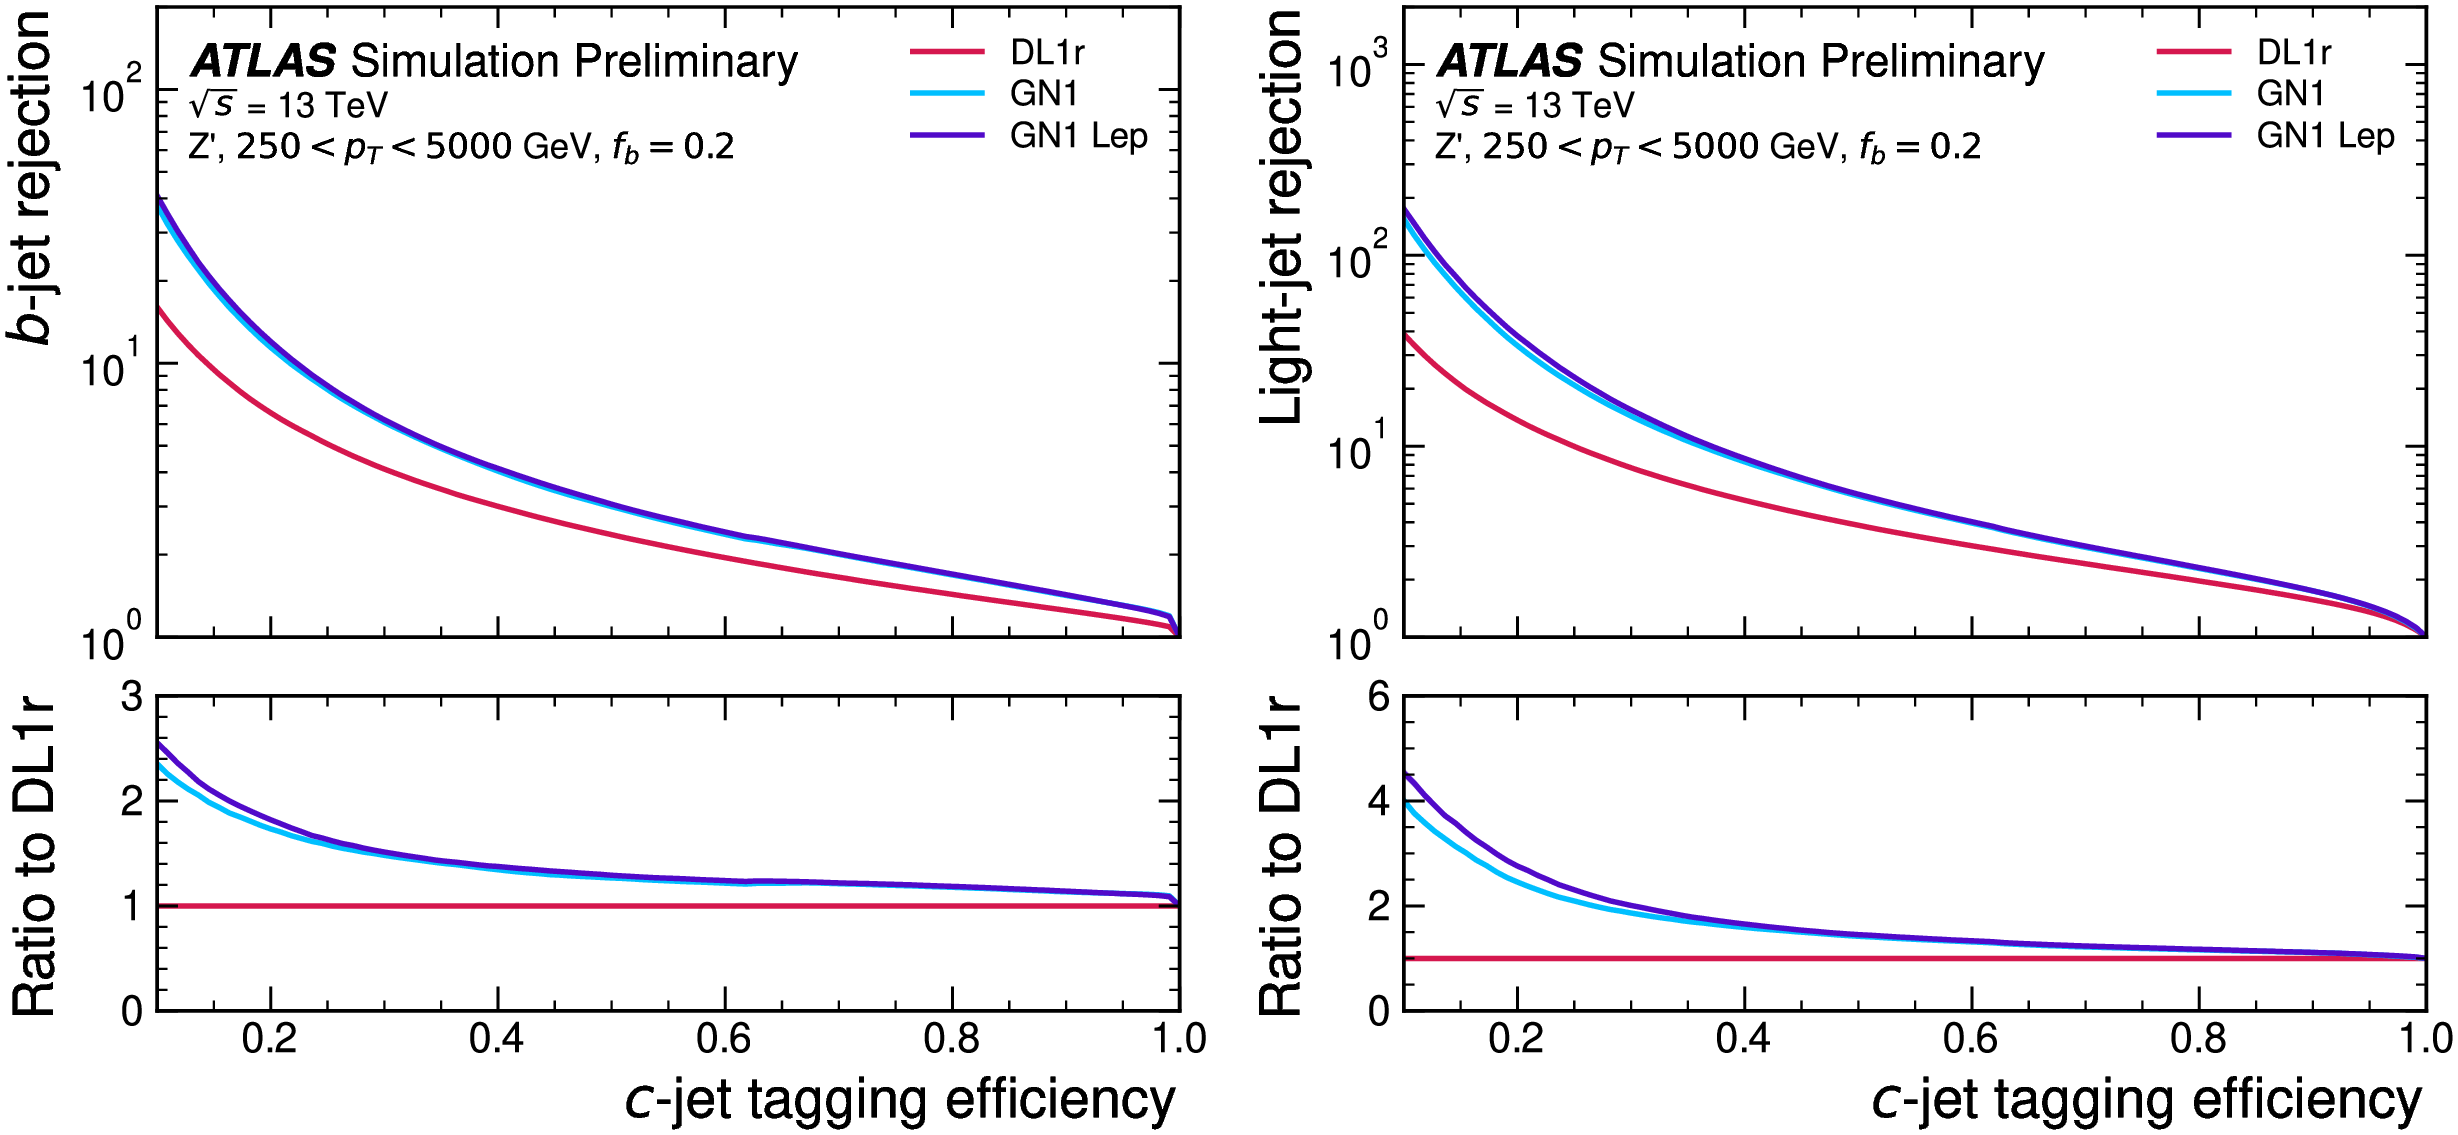
\includegraphics[width=0.98\textwidth]{Images/FTAG/GN/GN1/ROC/zpc.png}
      \caption{GN1 performance on the $Z'$ test sample, with $250 < p_T < 5000$ GeV.} 
      \label{fig:GN1zpc}
  \end{subfigure}
  \caption{ROC curves tracing the $c$-tagging efficiency versus the $b$-jet (left) and light-jet (right) rejections for the $t\bar{t}$ (top) and $Z'$ (bottom) test samples \cite{ATL-PHYS-PUB-2022-027}. Models compared are DL1r in red, GN1 in blue, and GN1 Lep in purple. The bottom panels show the ratio to DL1r. The flavour fraction is set at $f^c_b = 0.2$. The binomial error bands are shown as shaded regions.}
  \label{fig:GN1rocc}
\end{figure} 

\begin{figure}[h!]
  \centering
  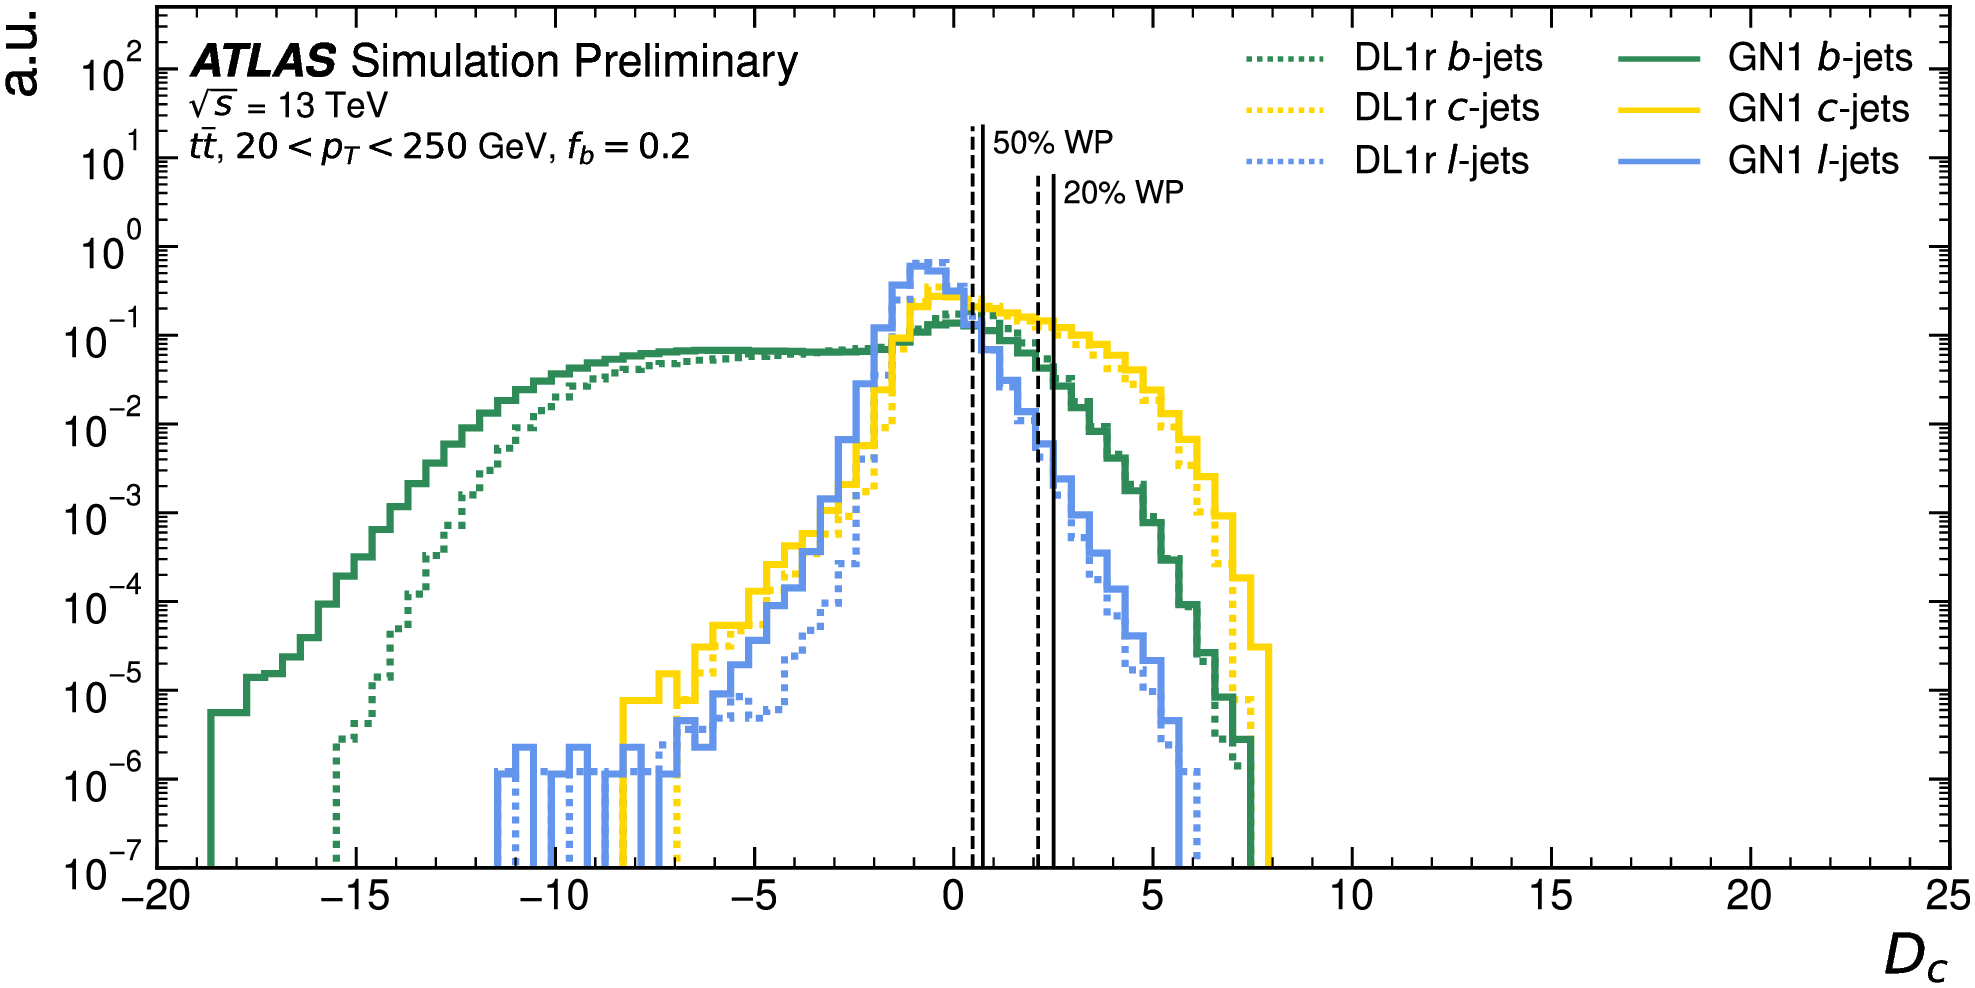
\includegraphics[width=0.8\textwidth]{Images/FTAG/GN/GN1/eff/ttc.png}
  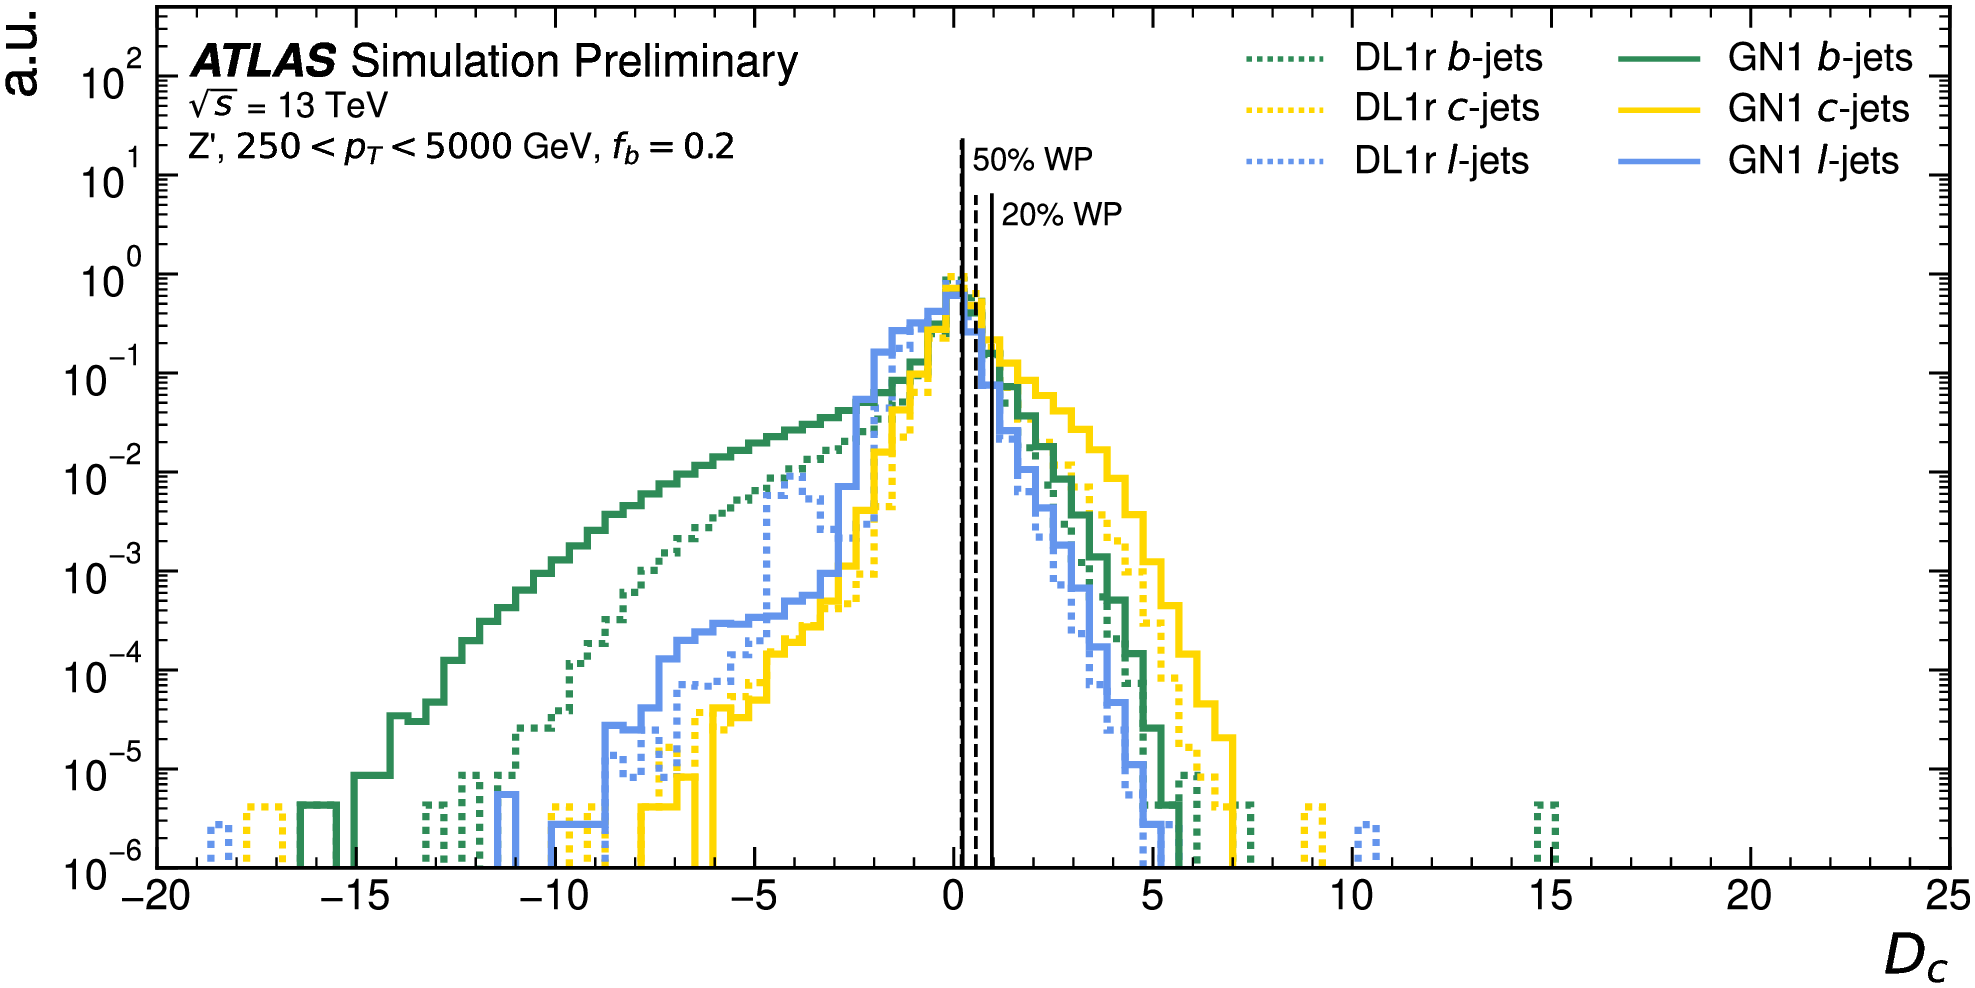
\includegraphics[width=0.8\textwidth]{Images/FTAG/GN/GN1/eff/zpc.png}
  \caption{Comparing the GN1 and DL1r $c$-tagging discriminants $D_c$ normalised distributions on the $t\bar{t}$ (top) and $Z'$ (bottom) test samples \cite{ATL-PHYS-PUB-2022-027}. Models compared are DL1r in dashed lines and GN1 in continuous lines. Each flavour is indicated by a different colour: green for $b$-jets, yellow for $c$-jets, and blue for light-jets. The flavour fraction is set at $f^c_b = 0.2$.}
  \label{fig:GN1disc}
\end{figure} 

\begin{figure}[h!]
  \centering
  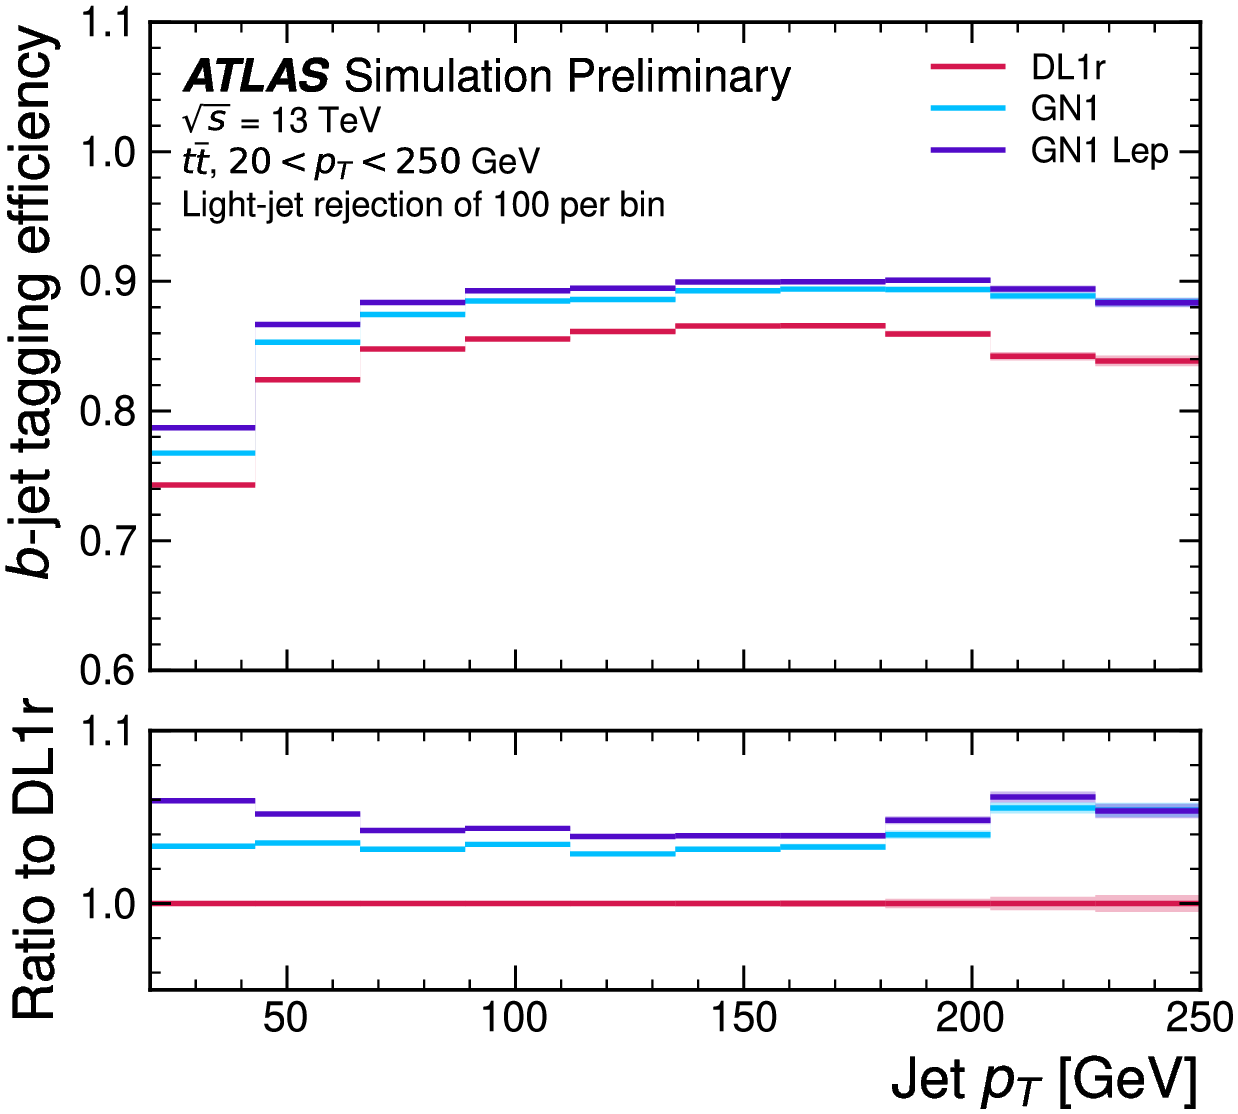
\includegraphics[width=0.45\textwidth]{Images/FTAG/GN/GN1/eff/ptttb.png}
  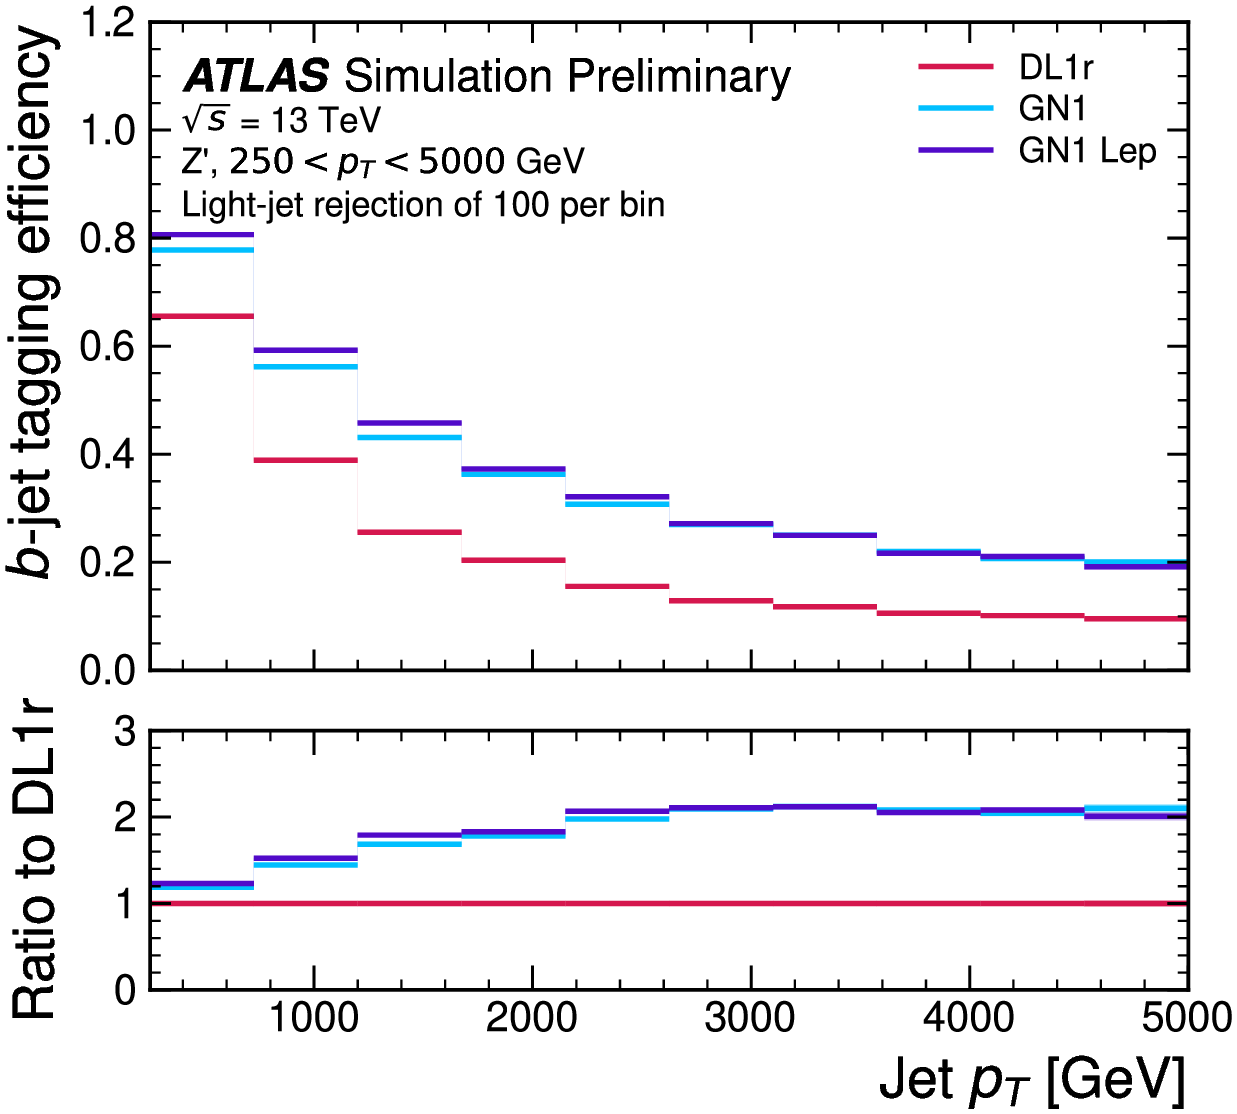
\includegraphics[width=0.45\textwidth]{Images/FTAG/GN/GN1/eff/ptzpb.png}
  \caption{Comparing the GN1 and DL1r $b$-tagging efficiency as a function of jet $p_T$ at a fixed 100 light-jet rejection in each bin on the $t\bar{t}$ (left) and $Z'$ (right) test samples \cite{ATL-PHYS-PUB-2022-027}. Models compared are DL1r in dashed lines and GN1 in continuous lines. The flavour fraction is set at $f^b_c = 0.018$ for DL1r and 0.05 for GN1 and GN1 Lep.}
  \label{fig:GN1ptb}
\end{figure} 

As previously highlighted, the tagging performance is strongly anti-correlated with the jet energy considered, explaining the observed rejection differences between the $t\bar{t}$ and $Z'$ samples. Higher energies correlate with higher transverse momentum $p_T$. More energy in the system introduces a higher multiplicity of fragmentation particles challenging the reconstruction process. The direction of emission of the particles is more collimated and approaches the resolution power of the tracking detector granularity. Different tracks are no longer individually resolvable and their hits are merged. Due to relativistic effects, the time of flight of heavy-hadrons increases at higher $p_T$, delaying their decay further into the depth of the detector. Traces left by the heavy-hadrons paths and fragmentation particles introduce inaccuracies in the reconstructed track parameters \cite{ATLAS-tracks-algo}. This degradation of the track quality impacts the jet tagging performance significantly, as displayed in Figure~\ref{fig:GN1ptb} showing the $b$-tagging efficiency as a function of jet $p_T$ for a fixed light-jet rejection of 100 in each bin. \gls{gn1} outperforms \gls{dl1r} across the studied $p_T$ spectrum, with a very significant $b$-efficiency improvement of a factor $\sim$ 2 at high values of $p_T$, above 2 TeV. \\

To conclude this section on \gls{gn1}, the importance of the auxiliary tasks is discussed by presenting ablations studies removing them iteratively from the full \gls{gn1} model. For this purpose, three variants of \gls{gn1} are trained equivalently to the full \gls{gn1}:
\begin{itemize}
  \item Without any auxiliary objectives, leading to a model labelled ``GN1 No Aux'' only optimising the jet classification objective.
  \item With only the vertexing auxiliary objective, for the model labelled ``GN1 Vert''.
  \item With only the track classification auxiliary objective, for the ``GN1 TC'' model.
\end{itemize}
Figure~\ref{fig:GN1ablb} displays the \gls{roc} curves of these modified models compared to the previously introduced \gls{dl1r} and the full \gls{gn1}. Removing the auxiliary objectives has a large impact on performance. The \gls{gn1} No Aux model is effectively similar to a \gls{dl1d} model, having similar performance gains with respect to \gls{dl1r}. Remarkably, this performance is obtained from a single network processing track without any of the subtagger nor methods used by the DL1 family, effectively underlying the powerful representation power of \gls{gat}. Adding either of the auxiliary tasks has the same beneficial impact on performance, as GN1 TC and GN1 Vert performs similarly and each is enough to significantly outmatch \gls{dl1r}. The real gain is obtained by adding both auxiliary tasks, which further boosts the effectiveness of the model.\\

\begin{figure}[h!]
  \centering
  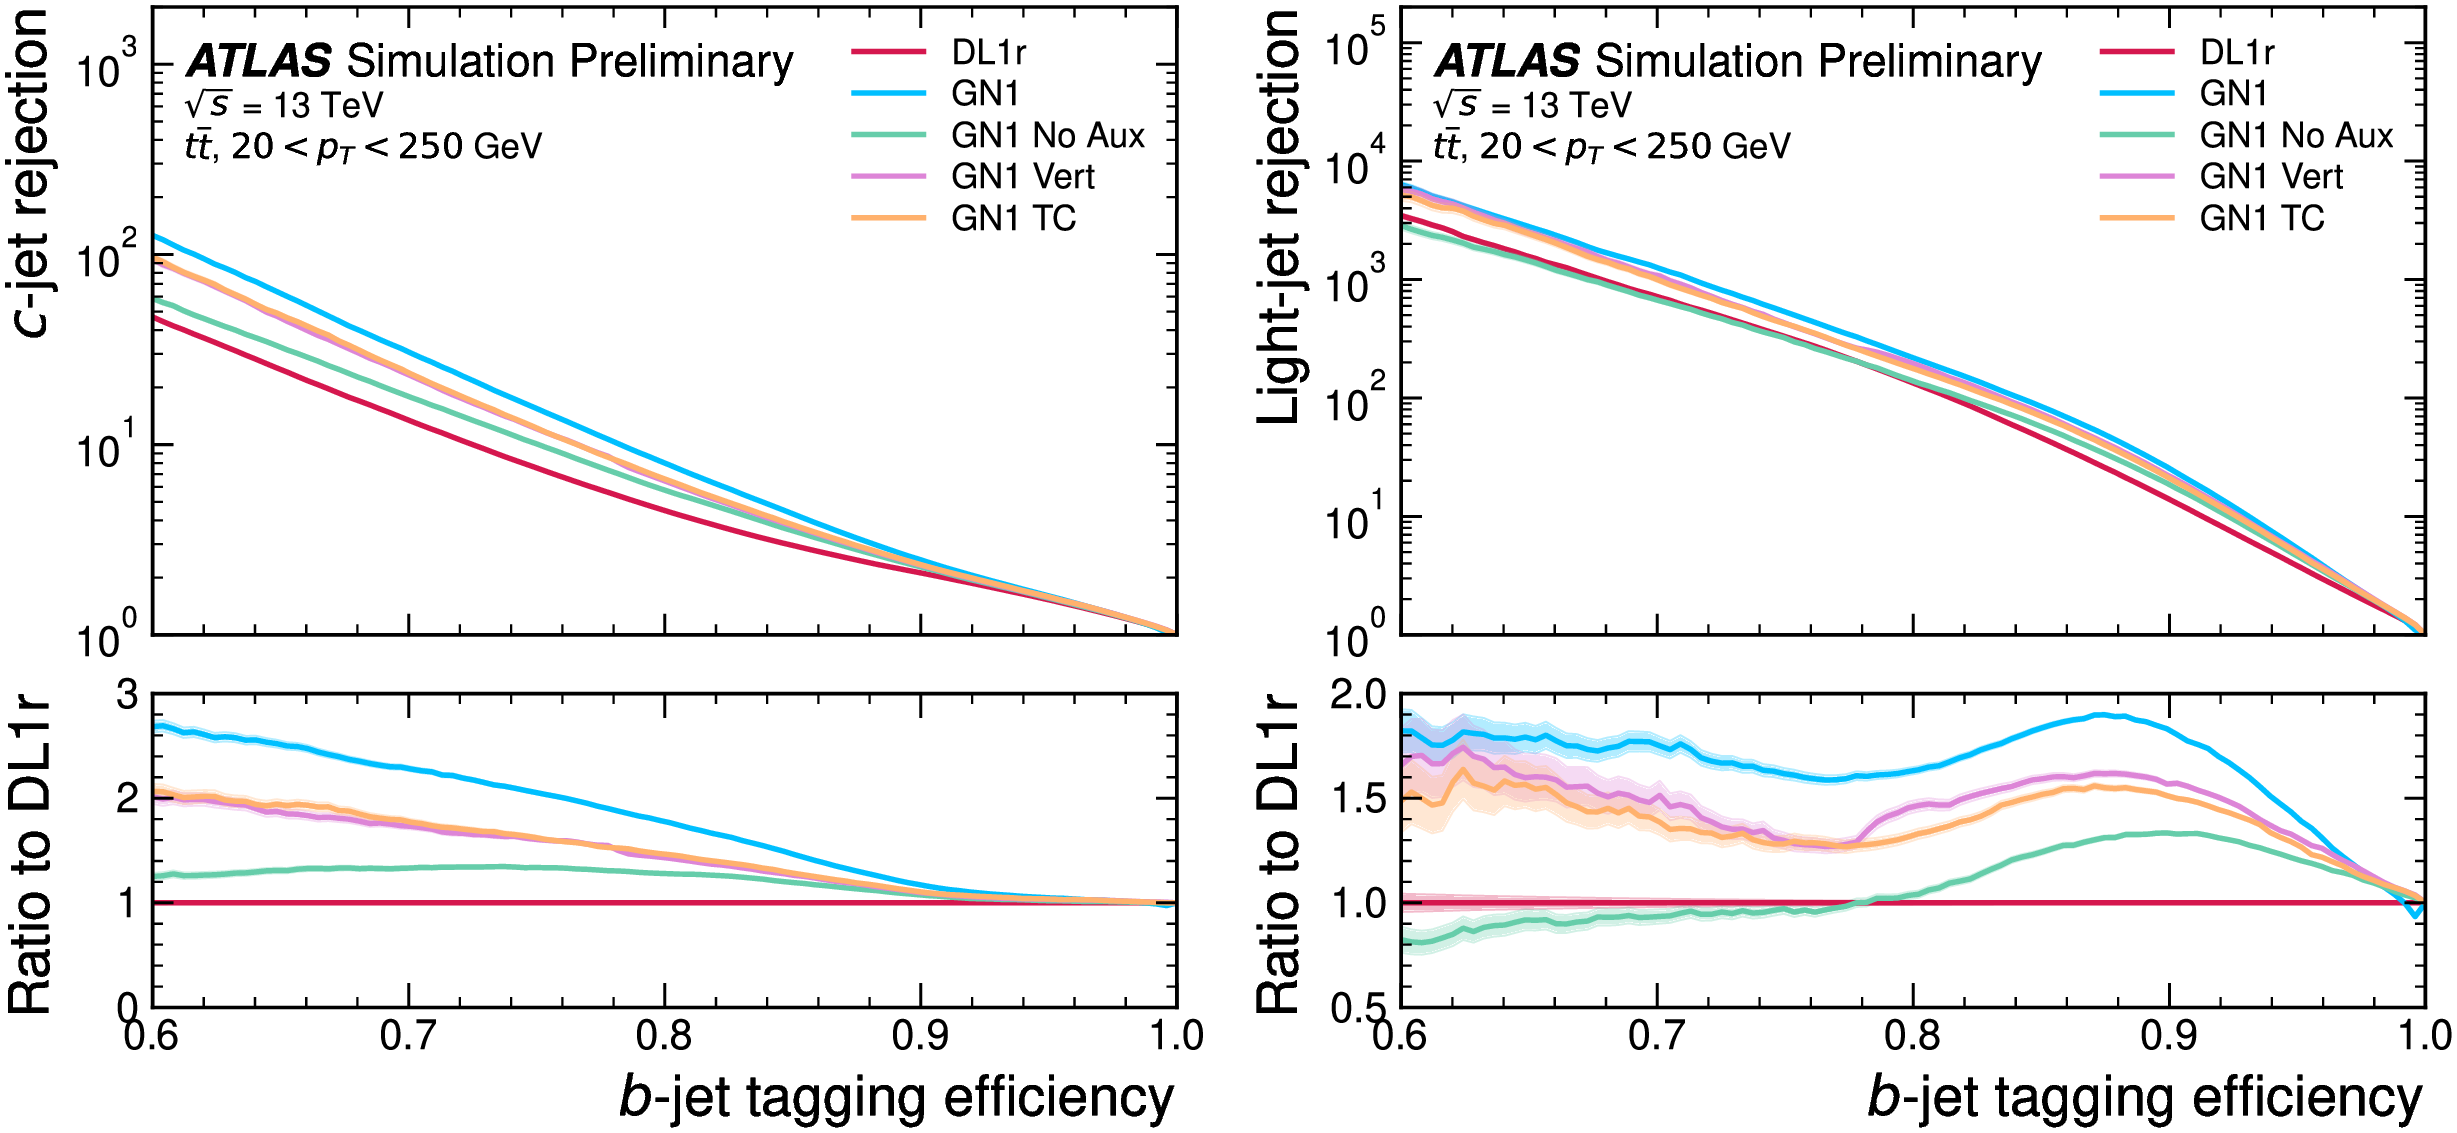
\includegraphics[width=0.98\textwidth]{Images/FTAG/GN/GN1/ablations/ttb.png}
  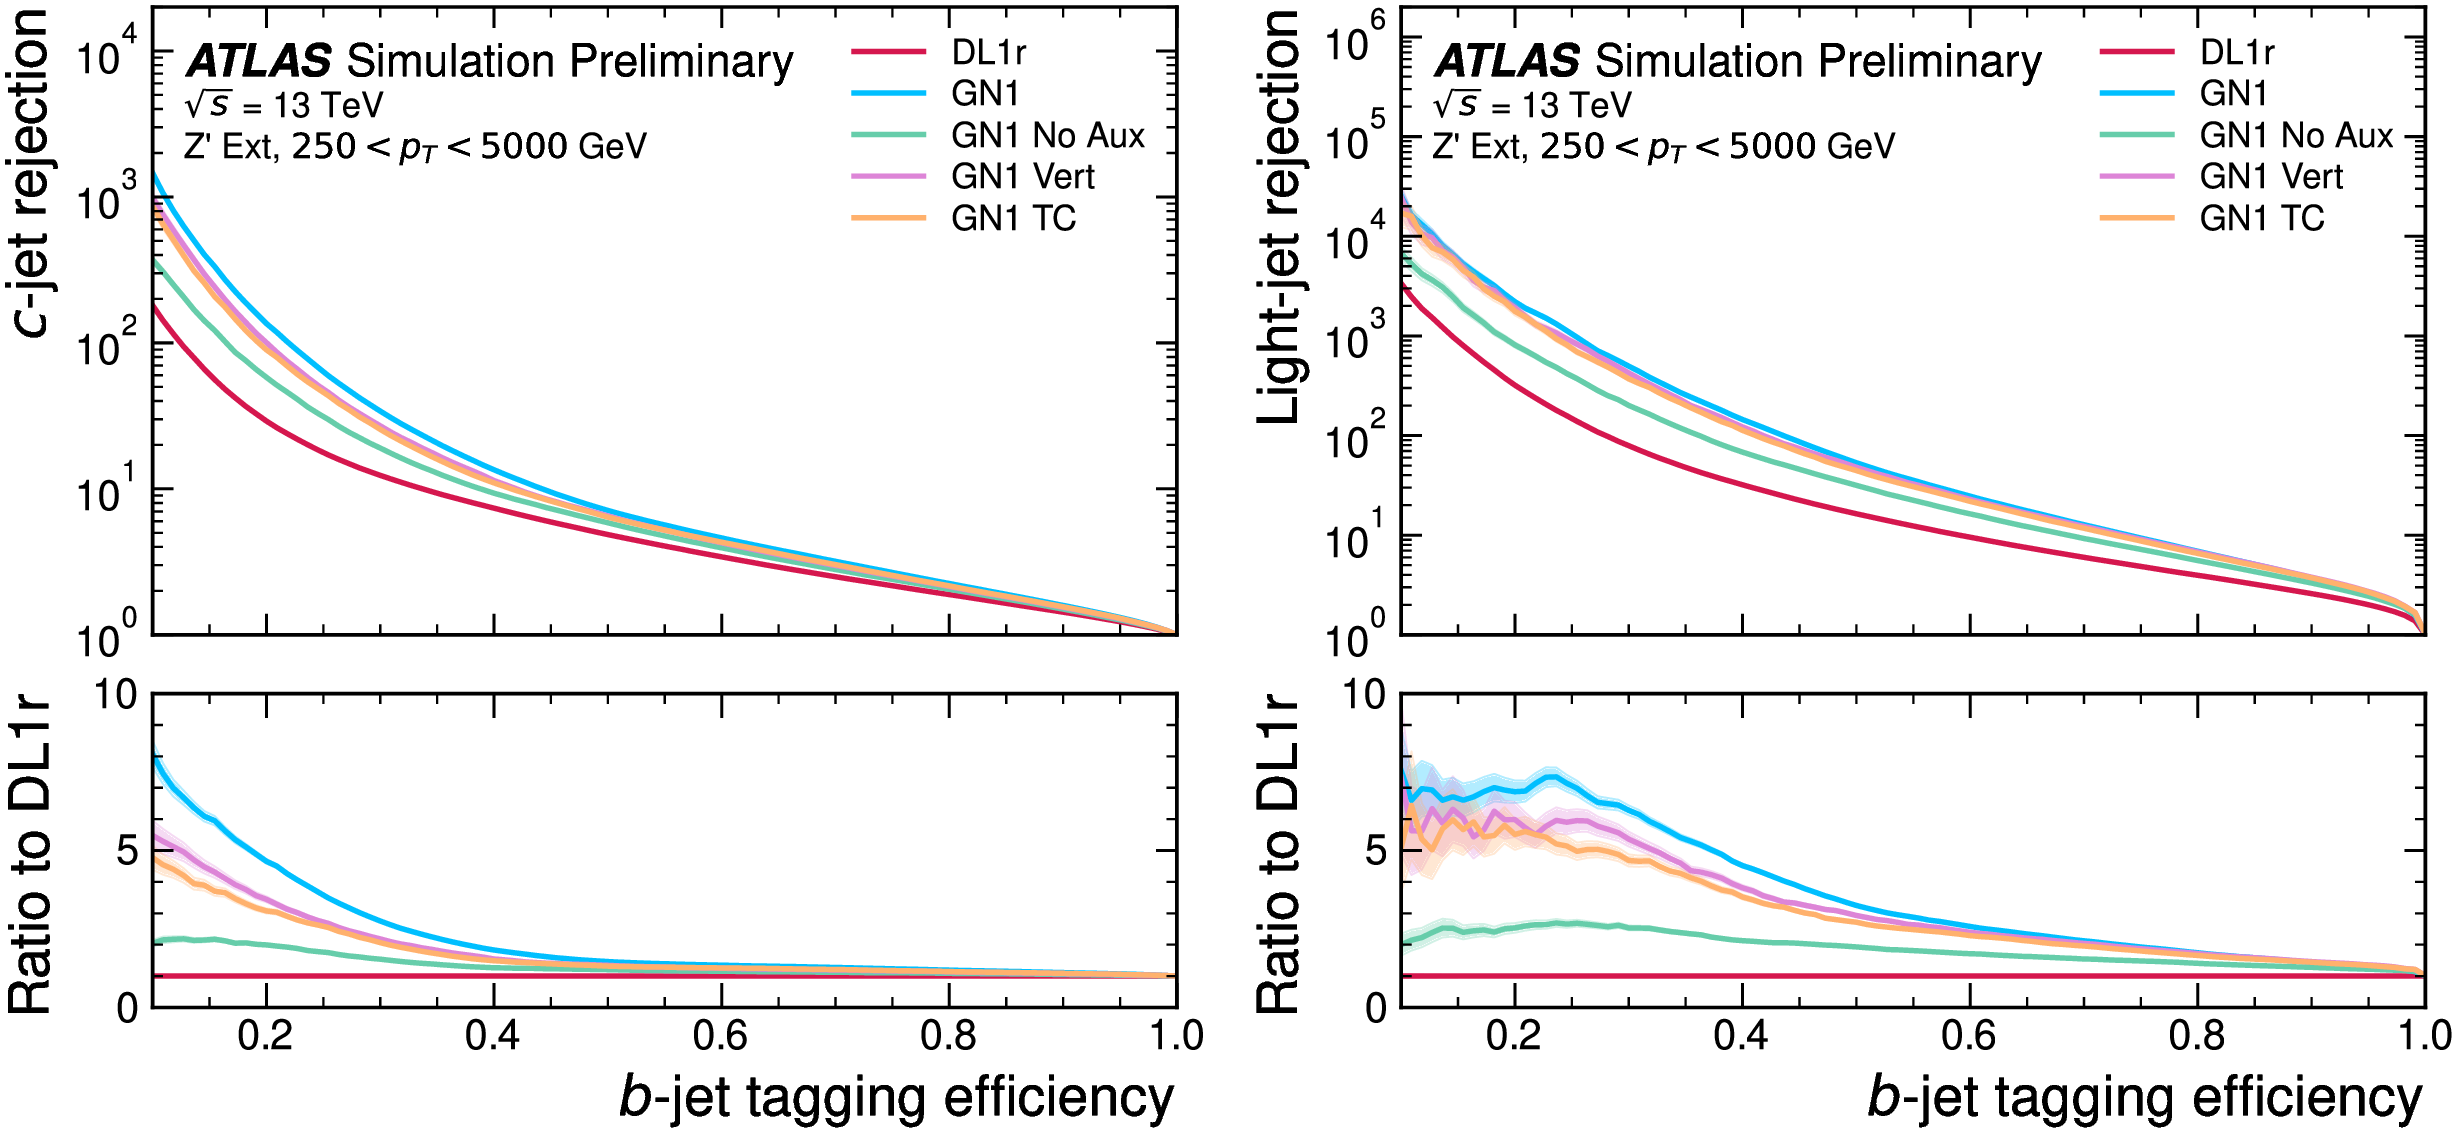
\includegraphics[width=0.98\textwidth]{Images/FTAG/GN/GN1/ablations/zpb.png}
  \caption{ROC curves tracing the $b$-tagging efficiency versus the $c$-rejection (left) and light-rejection (right) for the $t\bar{t}$ (top) and $Z'$ (bottom) test samples \cite{ATL-PHYS-PUB-2022-027}. Models compared are DL1r in red, GN1 in blue, and versions of GN1 with missing auxiliary tasks. GN1 No Aux in green has none of the auxiliary, GN1 Vert in purple only the vertexing task, and GN1 TC in orange only the track classification. The flavour fraction is set at $f^b_c = 0.018$ for DL1r and 0.05 for GN1. The binomial error bands are shown as shaded regions.}
  \label{fig:GN1ablb}
\end{figure} 

\paragraph{}So far, the performance of \gls{gn1} on the primary objective of jet flavour classification has been discussed. The performance on the auxiliary objectives is not directly relevant as they are only there to distil information to help the primary goal. The track-pairs vertexing performance can be assessed by leveraging the information to perform vertex finding: grouping sets of tracks that are found to share a vertex into a single reconstructed vertex. The result is compared to the truth vertex label available in the simulations. Vertices identified by \gls{gn1} as containing tracks coming from a $b$-hadron decay are grouped, and the same procedure is applied to the truth information. To measure performance, the reconstructed and true vertices are compared as well as the number of tracks correctly assigned. A vertex is correctly identified when it contains at least 65\% of the correct tracks with a purity of at least 50\%. The comparison is only carried out for reconstructed tracks, meaning a 100\% \gls{gn1} efficiency corresponds to correctly identifying all possible secondary vertices within the limit of the track reconstruction efficiency. An inclusive reconstruction efficiency in $b$-jets of $\sim$80\% is measured for \gls{gn1}, effectively proving that the model can identify $b$-hadron decay vertices. An important caveat is the current restriction is only on finding such vertices, not on reconstructing them. To implement a fully-fledged secondary vertex fitter as an auxiliary objective, the fitting of the vertex must be produced by a differentiable algorithm to allow for backpropagation. This is a promising area of research, given the physics-based interest in accessing this important \gls{sv} information. A promising example from Ref. \cite{smith2023differentiable} is under study to introduce an auxiliary differentiable single vertex fitting task in ATLAS. \\

\begin{figure}[h!]
  \centering
  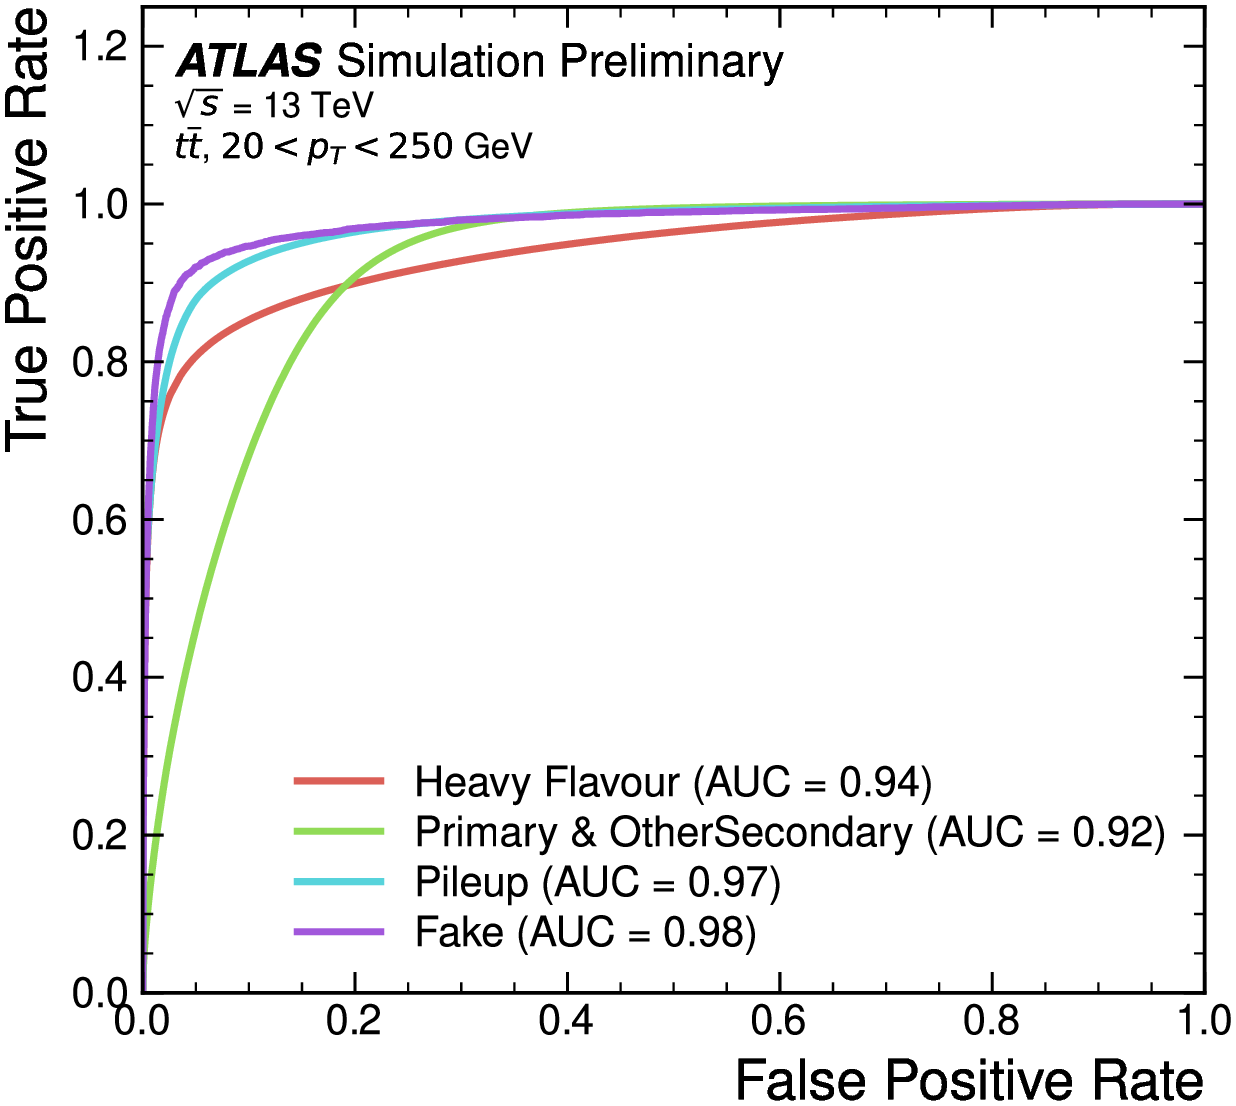
\includegraphics[width=0.48\textwidth]{Images/FTAG/GN/GN1/ablations/ttroc.png}
  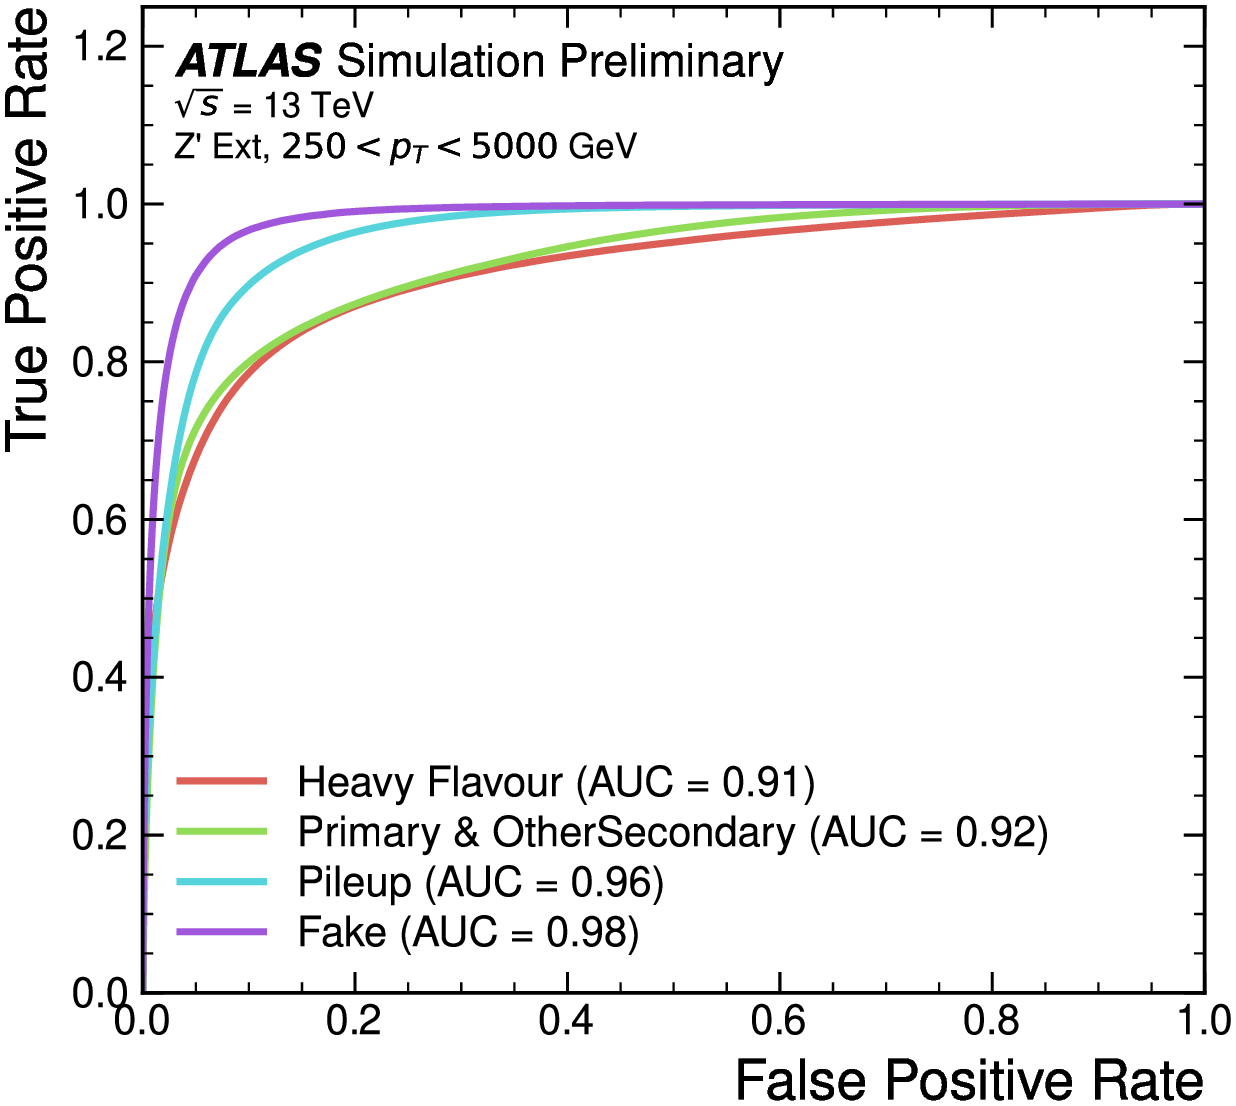
\includegraphics[width=0.48\textwidth]{Images/FTAG/GN/GN1/ablations/zproc.png}
  \caption{ROC curves tracing the false positive rate versus the true positive rate of the truth origin classification on the $t\bar{t}$ (left) and $Z'$ (right) test samples \cite{ATL-PHYS-PUB-2022-027}. Heavy Flavour is a weighted combination of the FromB, FromBC, and FromC by their relative abundance.}
  \label{fig:GN1trackperf}
\end{figure} 

Concerning the track origin classification performance, Figure~\ref{fig:GN1trackperf} presents some \gls{roc} curves, comparing the false positive rate (tracks wrongly assigned a label) versus the true positive rate (tracks correctly assigned a label), for the different track origin classes of Table~\ref{tab:gnTrackOrigin}. Some classes are combined with weights dictated by the subclass relative abundance: this is the case of the FromB, FromBC, and FromC classes that are combined as Heavy Flavour, and the Primary and OtherSecondary labels. The \gls{auc} of the \gls{roc} of all groups is above 90\%, indicating good classification performance. The most challenging categories are the Heavy Flavour, Primary, and OtherSecondary tracks, while the Fake and Pileup tracks are effectively identified. The global mean (weighted) \glspl{auc} are of 92\% (95\%) on $t\bar{t}$ and 94\% (96\%) on $Z'$ \cite{ATL-PHYS-PUB-2022-027}. This performance ranking is in line with a physics-based intuition, and the $p_T$ effect can be noted by the reduction in \gls{auc} for the Heavy Flavour tracks on the $Z'$ sample. \\

\gls{gn1} shows clear benefits in moving away from the previous recipe to build taggers by combining several subalgorithms and methods with physics meaning. Embracing modern advanced machine learning, it underlines the superiority of a single network built around an advanced core unit. While the inner workings of the model are somewhat less interpretable than the previous DL1 family of taggers, expert knowledge is passed to the network thanks to the multitasking paradigm. %Building on this success, an upgraded architecture was quickly developed to accelerate the speed of training and continue pushing the performance of the method ever higher: \gls{gn2}.

\subsection{GN2: Transformer Encoder for Flavour Tagging}\label{chap-GN2}
\gls{gn2} is a fine-tuned modification of \gls{gn1} built with the same conceptual processing chain but easier to train and simpler to scale in parameters. The main modification with respect to \gls{gn1} is the replacement of the computationally complex and expensive \gls{gat} layers by a now ubiquitous architecture in machine learning: the transformer \cite{NIPS_transformerPaper}. As described in Chapter \ref{sec:transformer}, transformers are remarkably effective, both able to extract fine-grained correlations between ordered and unordered tokens in a sequence through the mechanism of attention and to scale to very large network sizes without suffering from overtraining. By design, transformers combine rich attention-computing and regularisation-inducing steps letting these networks scale significantly their number of parameters while guaranteeing effective parallelisable training on \gls{gpu} hardware.  \\

\begin{table}[h]
  \begin{center}
      \begin{tabular}{c|c|c|c} 
      	 \hline \hline
          Modification & Parameter & GN1 & GN2 \\ \hline
          Hyperparameter  & Trainable parameters & 0.8M & 1.5M \\ 
          Hyperparameter  & Learning rate & Fixed 1e-3 & One-cycle scheduler\\ 
          Hyperparameter  & Core unit layers & 3 & 6 \\ 
          Hyperparameter  & Attention heads & 2 & 8 \\ 
          Hyperparameter  & Embedding dimension & 128 & 192 \\ \hline
          Architecture    & Attention Type & \gls{gat}v2 & Scaled dot product \\ 
          Architecture    & Dense update & No & Yes (dim 256) \\ 
          Architecture    & Separate value projection & No & Yes \\ 
          Architecture    & LayerNorm + Dropout & No & Yes \\ \hline
          Inputs          & Number of training jets & 30M & 192M  \\ \hline \hline
      \end{tabular}
    \caption{Main modifications between GN1 and GN2 \cite{ATL-PLOT-FTAG-2023-01}.}
    \label{tab:gn2compGN1}
  \end{center}
\end{table}

In the case of \gls{gn2}, the design only requires building a global representation of the sets of tracks composing a jet, hence only the encoder part introduced in Ref. \cite{NIPS_transformerPaper} and modified in Ref. \cite{shleifer2021normformer} is deployed to replace the \gls{gat} component of Figure~\ref{fig:ftagArchi}. A summary of the modifications adopted when switching from \gls{gn1} to \gls{gn2} is presented in Table~\ref{tab:gn2compGN1}. The reference to \gls{gn1} corresponds to the last version of the model that was developed, which already adopted some minor modifications to the \gls{gn1} model previously described. Similarly, the \gls{gn2} model described here corresponds to the first publically released model, and this generation is also being refined and improved at the time of writing this thesis. Some significant changes adopted for \gls{gn2} are a learning rate scheduler, a larger embedding space dimension giving a wider and deeper - thanks to the doubling of the number of layers - core transformer unit, and the introduction of regularising effects from layer normalisation and dropout \cite{ba2016layer}. The learning rate scheduler is based on the one-cycle scheduler of Ref.~\cite{smith2018disciplined}, with some important parameters described in Table~\ref{tab:onecyclescheduler}. This scheduler speeds up the training by initially growing the learning rate to larger values, corresponding to larger steps in the optimisation landscape, before annealing progressively the learning rate to smaller values, helping the optimiser to converge to a specific minimum \cite{smith2018superconvergence}. The attention computation implemented by the transformer produces similar physics performance to the \gls{gat} at a reduced memory footprint and training time \cite{duperrin2023flavour}. The improved computational performance of \gls{gn2} allows to scale up the number of parameters of the network and the training dataset size. Consequently, \gls{gn2} has roughly twice as many parameters as \gls{gn1} and was trained on a much larger training dataset. \gls{gn2} can indeed be trained on roughly $\times 6$ more jets than \gls{gn1} with the same computing resources. The datasets for the \gls{gn2} training presented here are derived similarly to those previously introduced for \gls{dl1d} and \gls{gn1}, using importance sampling to fully utilise the $b$- and light-jets statistics. 

\begin{table}[h]
  \begin{center}
      \begin{tabular}{c|c} 
      	 \hline \hline
          Parameter   & Description \\ \hline
          LR initial  & Initial value of the learning rate   \\ 
          LR maximal  & Maximal value of the learning rate reached at the end of warm-up   \\ 
          LR final    & Value of the learning rate reached at peak epoch    \\ 
          Warm-up     & Period covering the increase from initial to maximal   \\ 
          Peak epoch  & Epoch at which LR maximal should be reached   \\ \hline \hline
      \end{tabular}
    \caption{The five parameters of the one-cycle scheduler.}
    \label{tab:onecyclescheduler}
  \end{center}
\end{table}

The attention mechanism in the transformer is subtly different from the \gls{gat} and corresponds to the multihead self-attention process described in Chapter \ref{sec:transformer}. The nodes are updated in two steps: first attention is computed and applied, then a dense layer updates the set of nodes. In more detail, the transformer implements the following update on the set of nodes $h_i \in \mathcal{N}$ defining the fully connected graph $G(\mathcal{N})$:
\begin{enumerate}
  \item Layer normalisation is applied to the input set of nodes $\mathcal{N}$.
  \item For each attention head, 3 individual mappings represented by layers $W_q$, $W_k$, and $W_v$ map each node $h_i \in \mathcal{N}$ to three independent representations $W_qh_i$, $W_kh_i$, and $W_vh_i$.
  \item For each node $h_i \in \mathcal{N}$, edge scores are computed with all nodes $h_j$ using the scaled dot product attention \[e\left(h_i, h_j\right) = \frac{W_q h_i\, . \, W_k h_j}{\sqrt{s}},\] where the $s$ parameter representing the scaling weight is typically taken to be the dimension of matrix $W_k$. 
  \item The edge scores are turned into attention scores for node $i$, by taking the softmax over all nodes: \[a_{i, j} = \textrm{softmax}_j\left(e(h_i, h_j) \right).\]
  \item Each node $h_i \in \mathcal{N}$ is updated into a node $h_i' \in \mathcal{N}'$ as: \[h_i' = \sum_j a_{i, j} \,.\, W_v h_j\]
  \item Using a skip connection, the updated nodes $\mathcal{N}'$ are added their original $\mathcal{N}$ values. 
  \item Layer normalisation is applied to the updated nodes $\mathcal{N}'$.
  \item The updated nodes are passed through a \gls{dnn}.
  \item The output of the \gls{dnn} is summed to the updated nodes by a skip connection.
\end{enumerate}

The \gls{gn2} model presented here combines 6 such transformer layers with 8 attention heads. A comparison of the global performance of this PFlow-trained \gls{gn2} model to the already introduced PFlow-trained \gls{dl1r}, \gls{dl1d}, and \gls{gn1} models is displayed in the $b$-tagging \gls{roc} curves of Figures \ref{fig:GN2rocb}. For this comparison, the \gls{gn2} and \gls{dl1d} models have been retrained on the same datasets, with the \gls{dl1r} and \gls{gn1} models equivalent to those presented in the previous section. \gls{gn2} delivers yet another significant boost in performance, drastically surpassing the \gls{gn1} rejections at all efficiencies considered. The largest improvement is obtained at lower $b$-jet efficiencies. Compared to \gls{gn1}, \gls{gn2} delivers $\times 1.5$ ($\times 1.7$) the $c$-rejection (light-rejection) on $t\bar{t}$ at the 70\% $b$-tagging \gls{wp} and $\times 1$ ($\times 1.7$) on $Z'$ at 30\% \gls{wp}. With respect to \gls{dl1d}, the gains in $c$-rejection (light-rejection) are respectively close to $\times 3$ ($\times 2$) for $t\bar{t}$ and $\times 3$ ($\times 4$) on $Z'$ at the same \gls{wp}. The $c$-rejection on $Z'$ of the GN models is essentially equivalent, although the significantly improved light-rejection of \gls{gn2} indicates its $c$-rejection can be boosted by further increasing its flavour fraction $f^b_c$ above 0.1. \\

Turning to $c$-tagging, as displayed in Figure~\ref{fig:GN2rocc}, a similar large performance gain is obtained by the new \gls{gnn} family over the DL1 one, both in terms of $b$- and light-rejection. \gls{gn2} introduces a large improvement on top of \gls{gn1}, although their $b$-rejection performance is equivalent on $Z'$. The gains from \gls{gn2} with respect to \gls{gn1} are of a factor $\times 1.3$ ($\times 1.3$) for $b$-rejection (light-rejection) on $t\bar{t}$ at the 30\% \gls{wp}, while they are $\times 1$ ($\times 1.2$) on $Z'$. The comparison to \gls{dl1d} is of $\times 1.9$ ($\times 2.1$) on $t\bar{t}$ and $\times 1.3$ ($\times 1.8$) on $Z'$, at the same \glspl{wp}. \\

Fixing the $b$-tagging performance at the 77\% \gls{wp} for both the $t\bar{t}$ and $Z'$, Figure~\ref{fig:GNxscansfc} scans the $f^b_c$ flavour fractions for the different models. A clear hierarchy of performance is observed: \gls{gn2} is orders of magnitude above the DL1 family and occupies undisputedly the highest rejections regions, followed by \gls{gn1}, \gls{dl1d}, and finally \gls{dl1r}. For $b$-tagging on $Z'$, the $c$-rejection can be further improved with limited impact on light-rejection by increasing $f^b_c$. However, the flavour fractions are optimised for an improved $c$-rejection on $t\bar{t}$, with limited change to the light-rejection across tagger generations. If desired, the light-rejection on $t\bar{t}$ of a \gls{gn2} taggers could be increased by lowering the $f^b_c$, reaching values as high as 1800 at a $c$-rej of 4.8. The maximal \gls{dl1d} light-rejection is 450 for a $c$-rejection of 4.5, thus a mere 25\% of the \gls{gn2} light-rejection. Similarly, \gls{gn2} can reach a $c$-rejection of 19.5 at a light-rejection of 110, compared to a maximal $c$-rejection of 9.7 at a light-rejection of 40. 

\begin{center}
  \begin{figure}[h!]
  \centerline{
  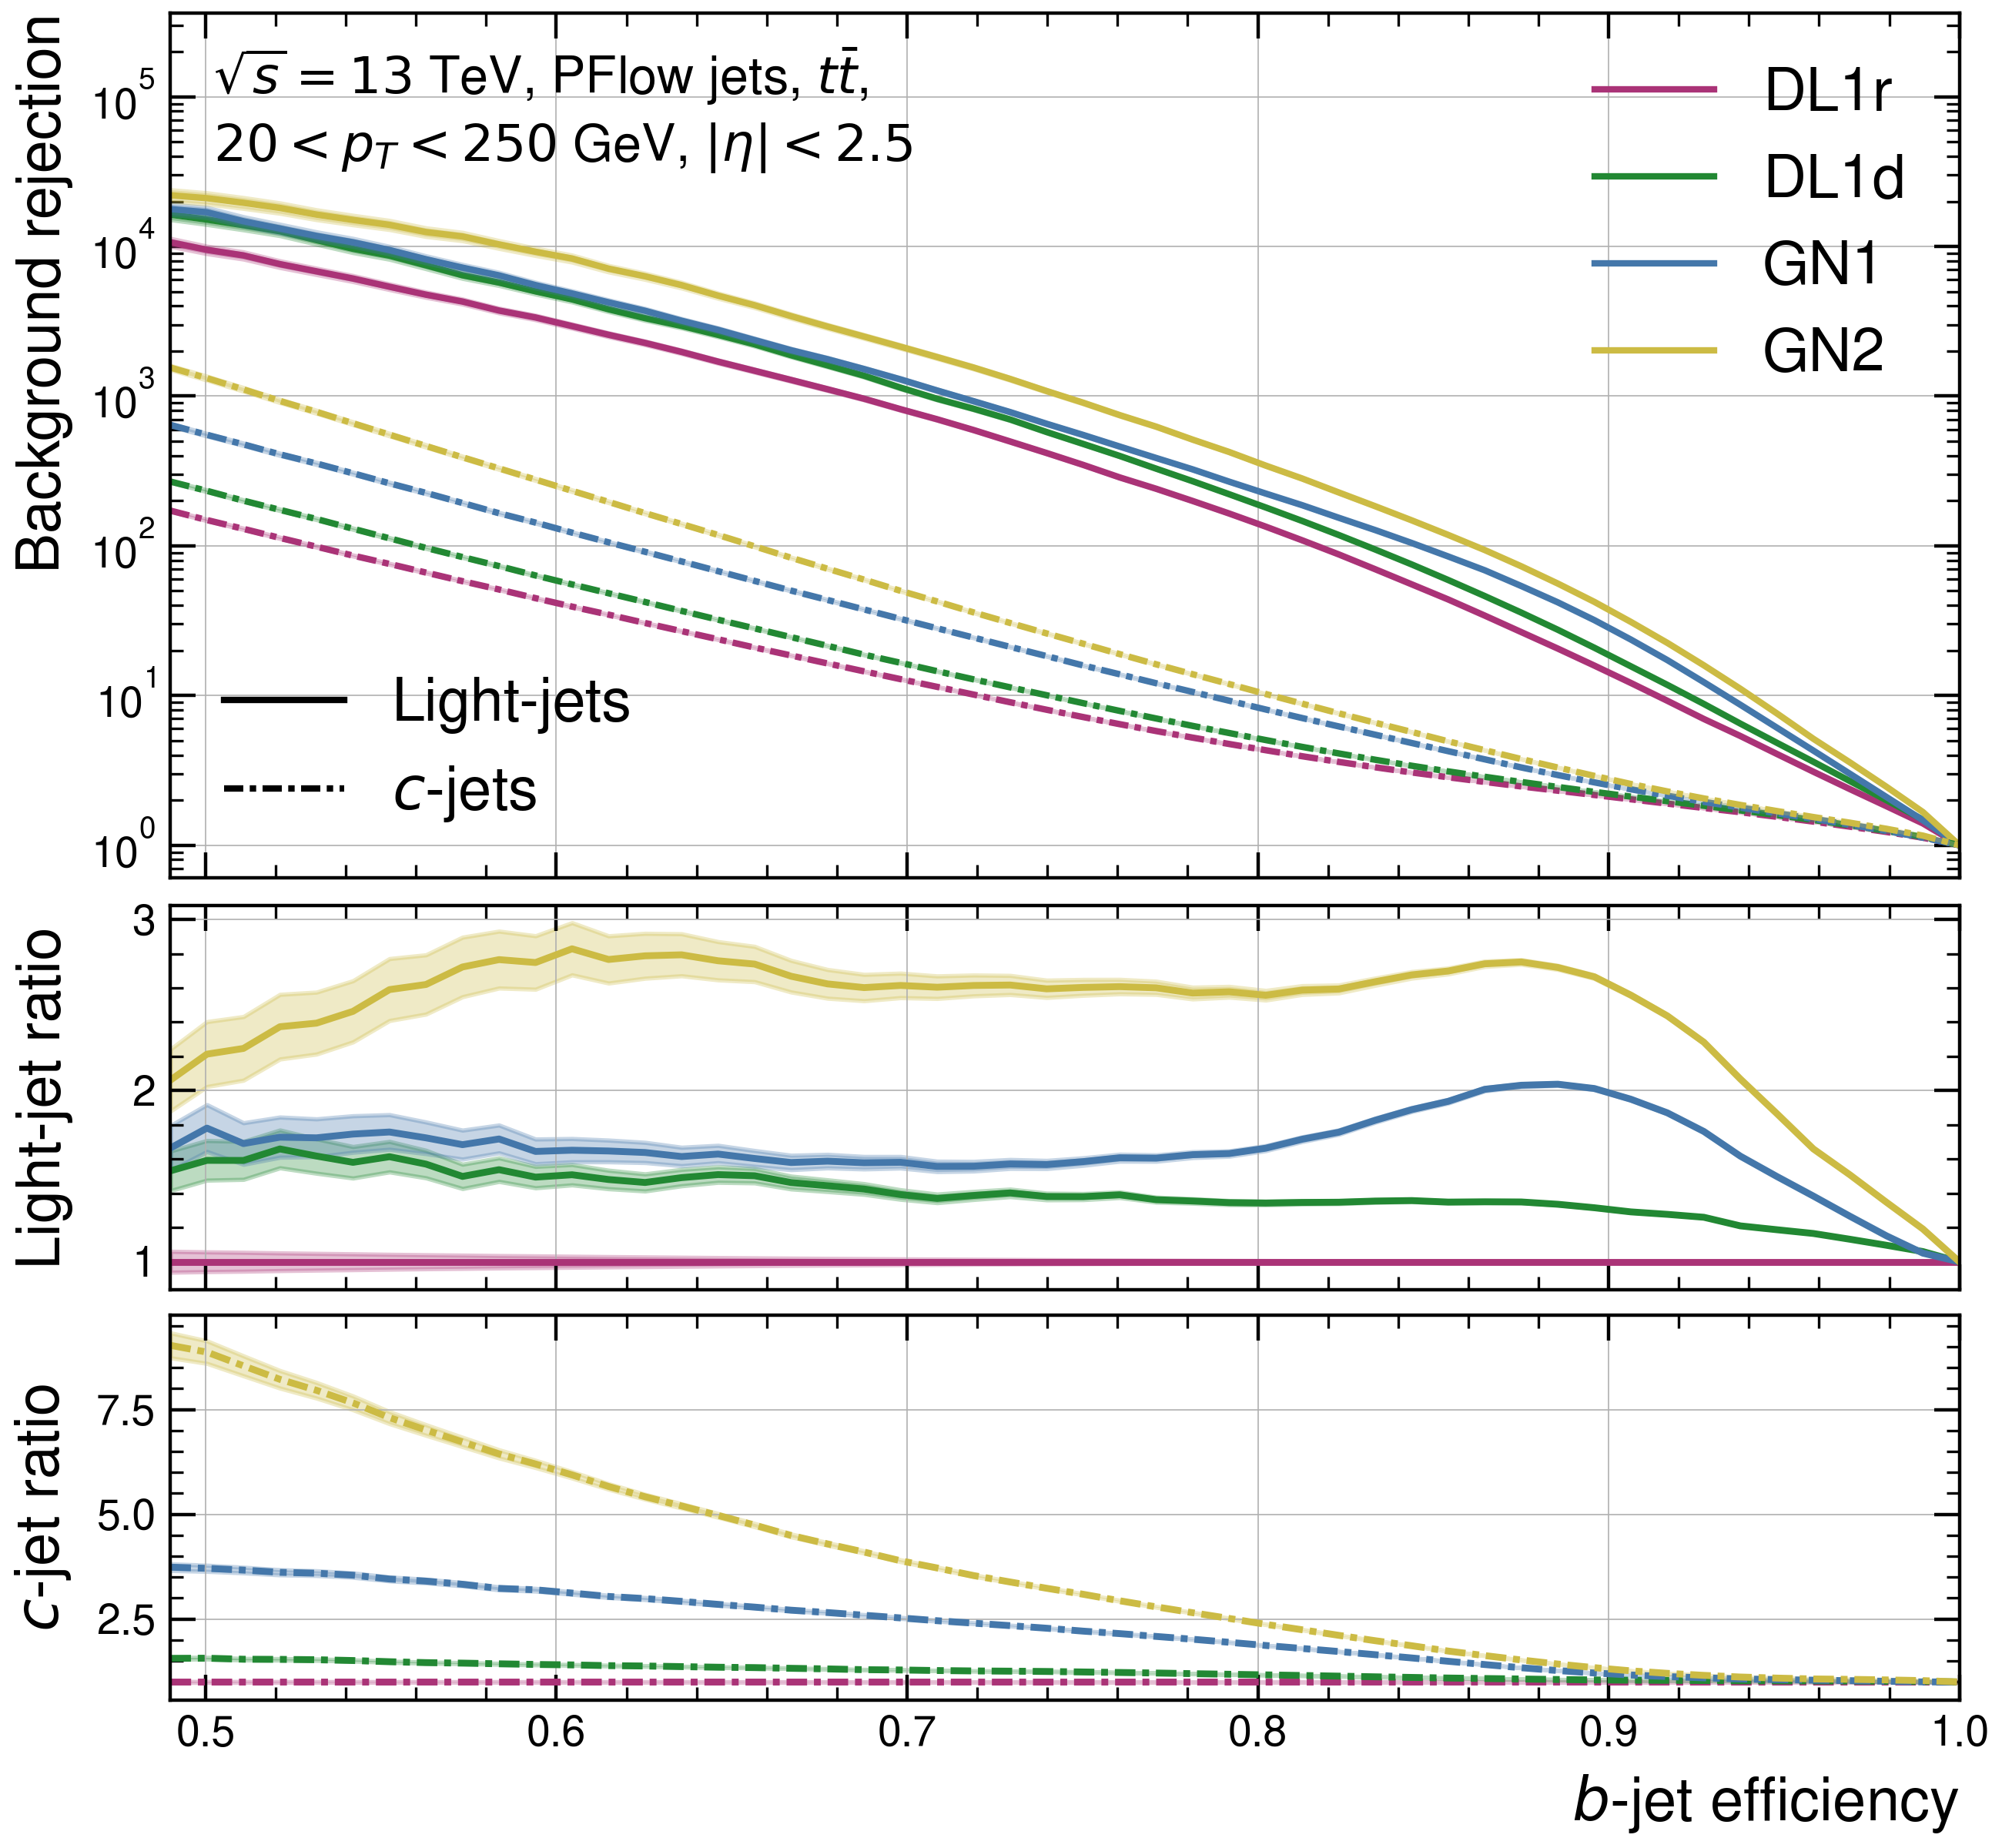
\includegraphics[width=0.50\textwidth]{Images/FTAG/GN/GN2/rocs/roc_ttbar.png}
  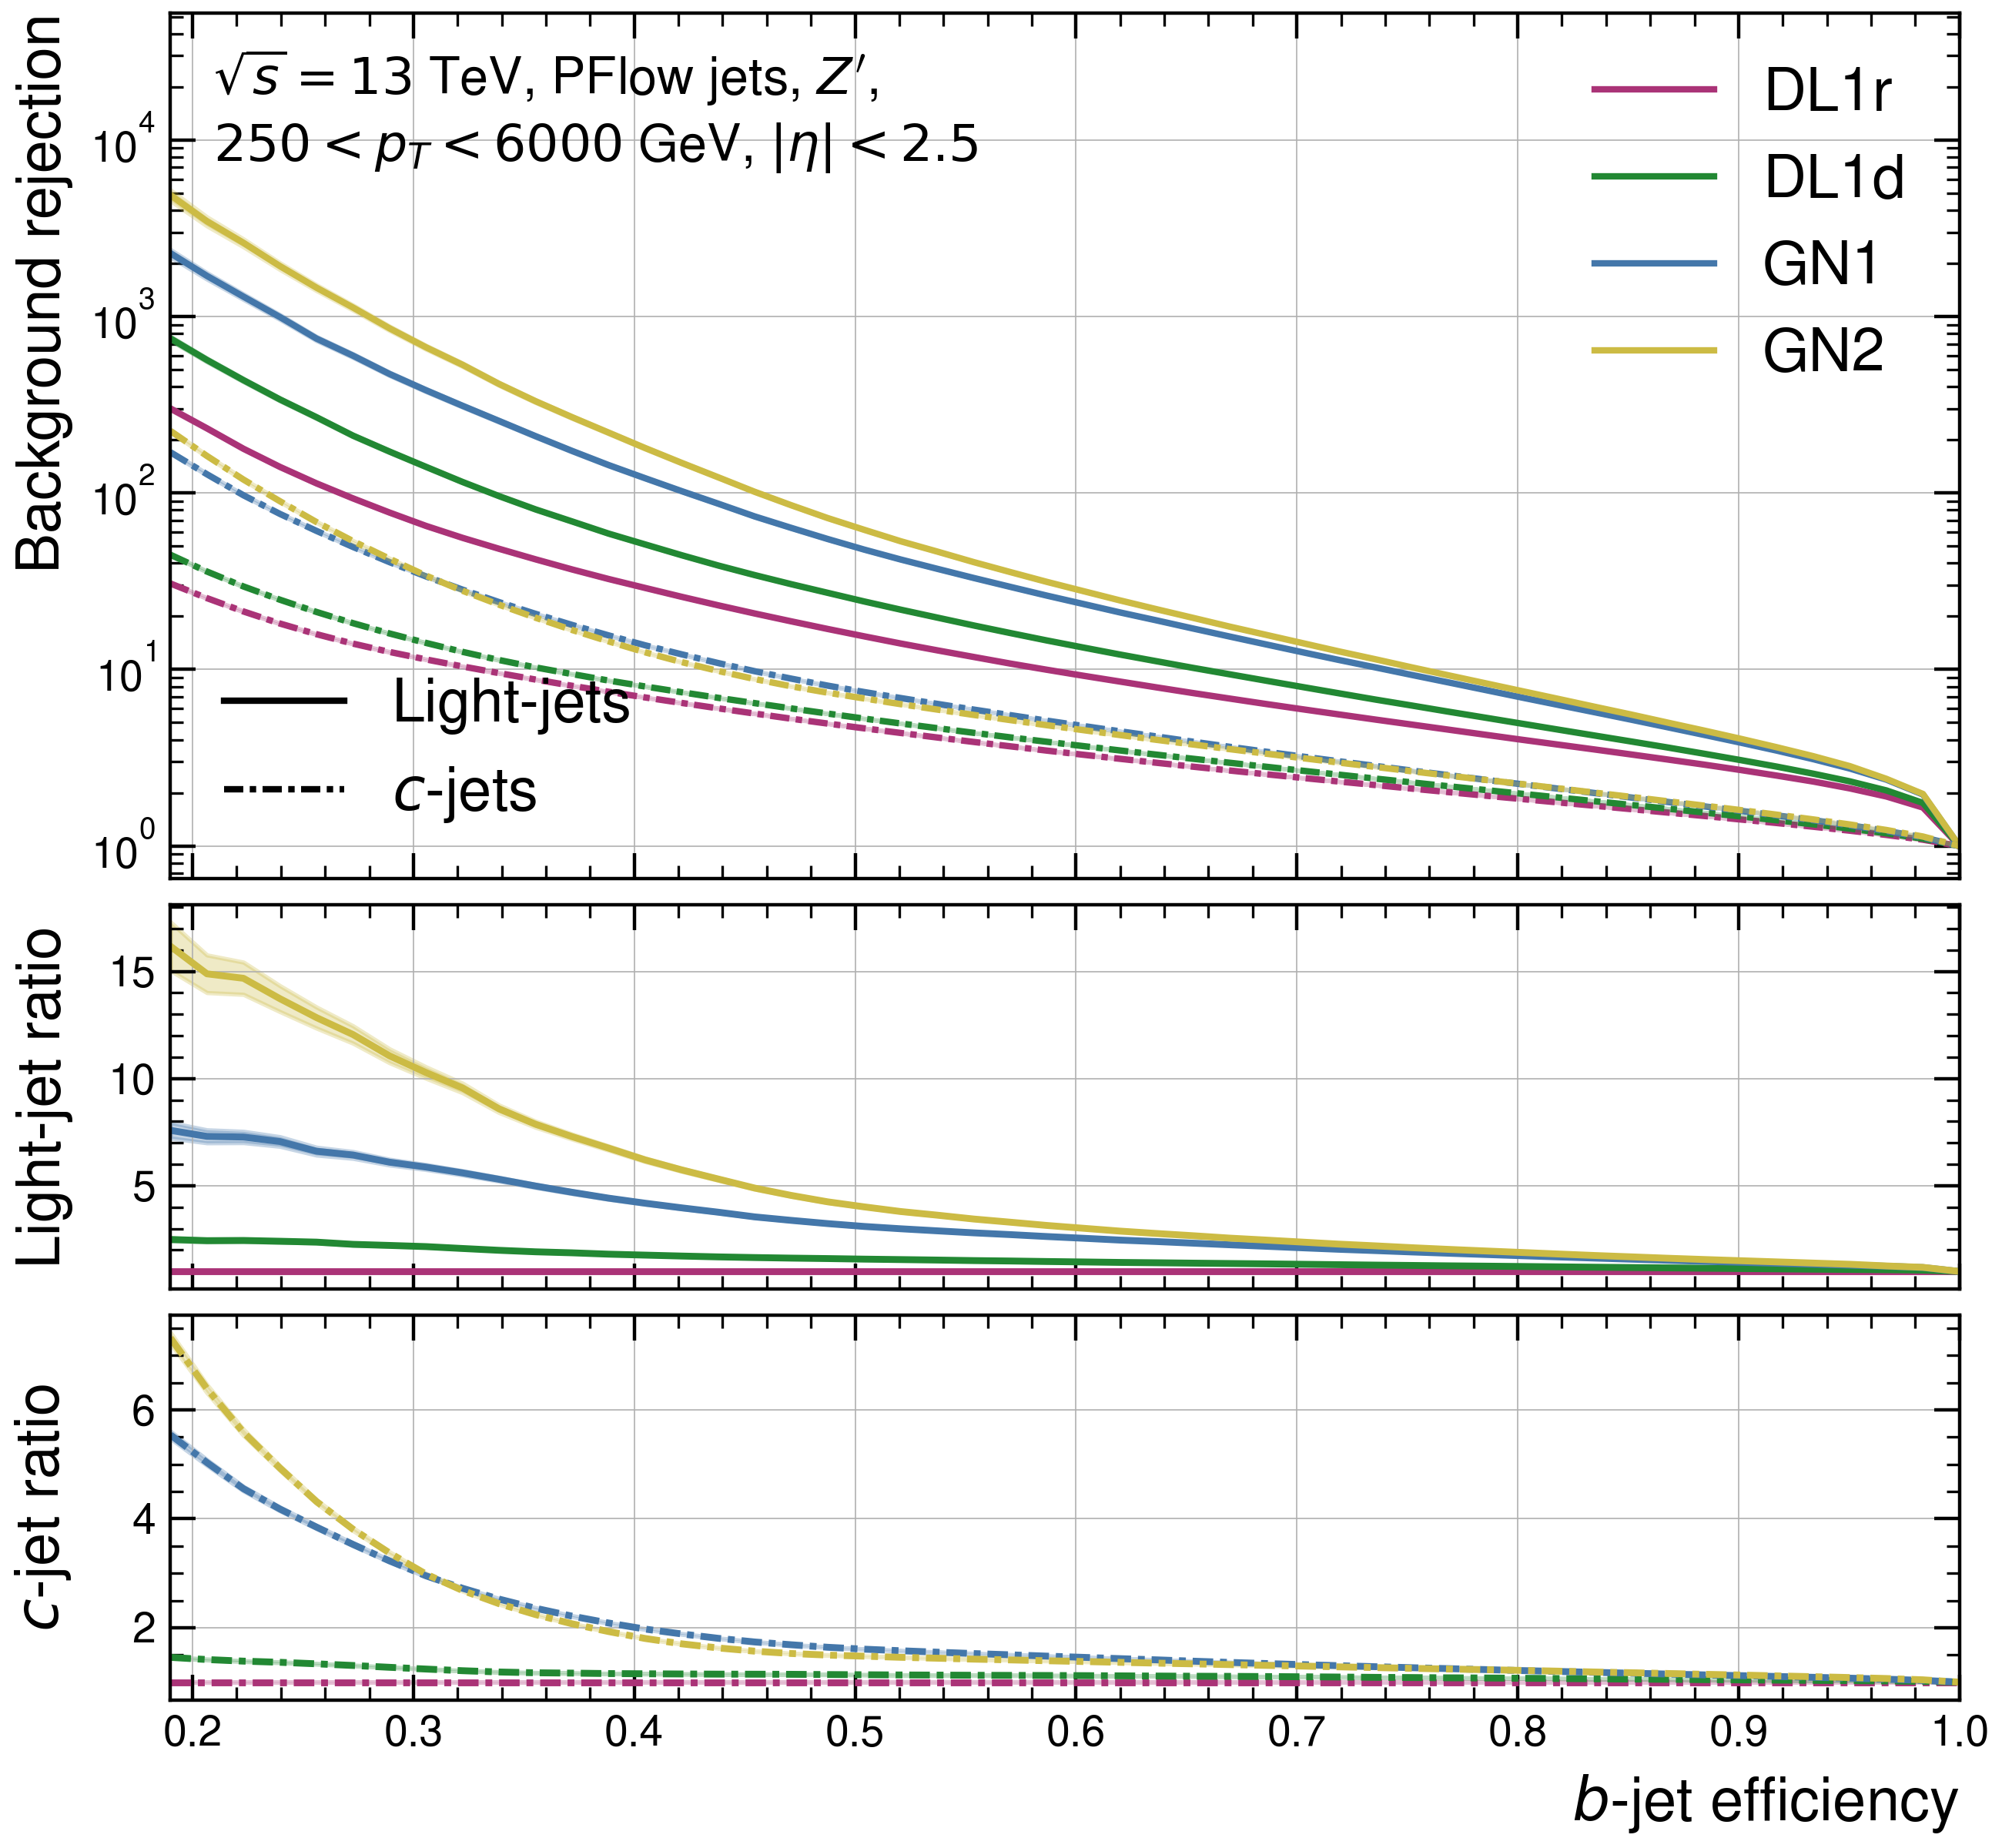
\includegraphics[width=0.50\textwidth]{Images/FTAG/GN/GN2/rocs/roc_zp.png}
  }
  \caption{The $c$- and light-rejections as a function of the $b$-jet tagging efficiency in the $t\bar{t}$ with $20 < p_T < 250$ GeV (left) and $Z'$ with $250 < p_T < 6000$ GeV (right) test samples. Models compared are DL1r in purple, DL1d in green, GN1 in blue, and GN2 in yellow. The bottom plots show the ratio to the DL1d performance. Flavour fractions are set at $f^b_c = 0.018$ for DL1r and DL1d, 0.05 for GN1, and 0.1 for GN2. Shaded regions represent the binominal error band.}
  \label{fig:GN2rocb}
  \bigskip
  \centerline{
  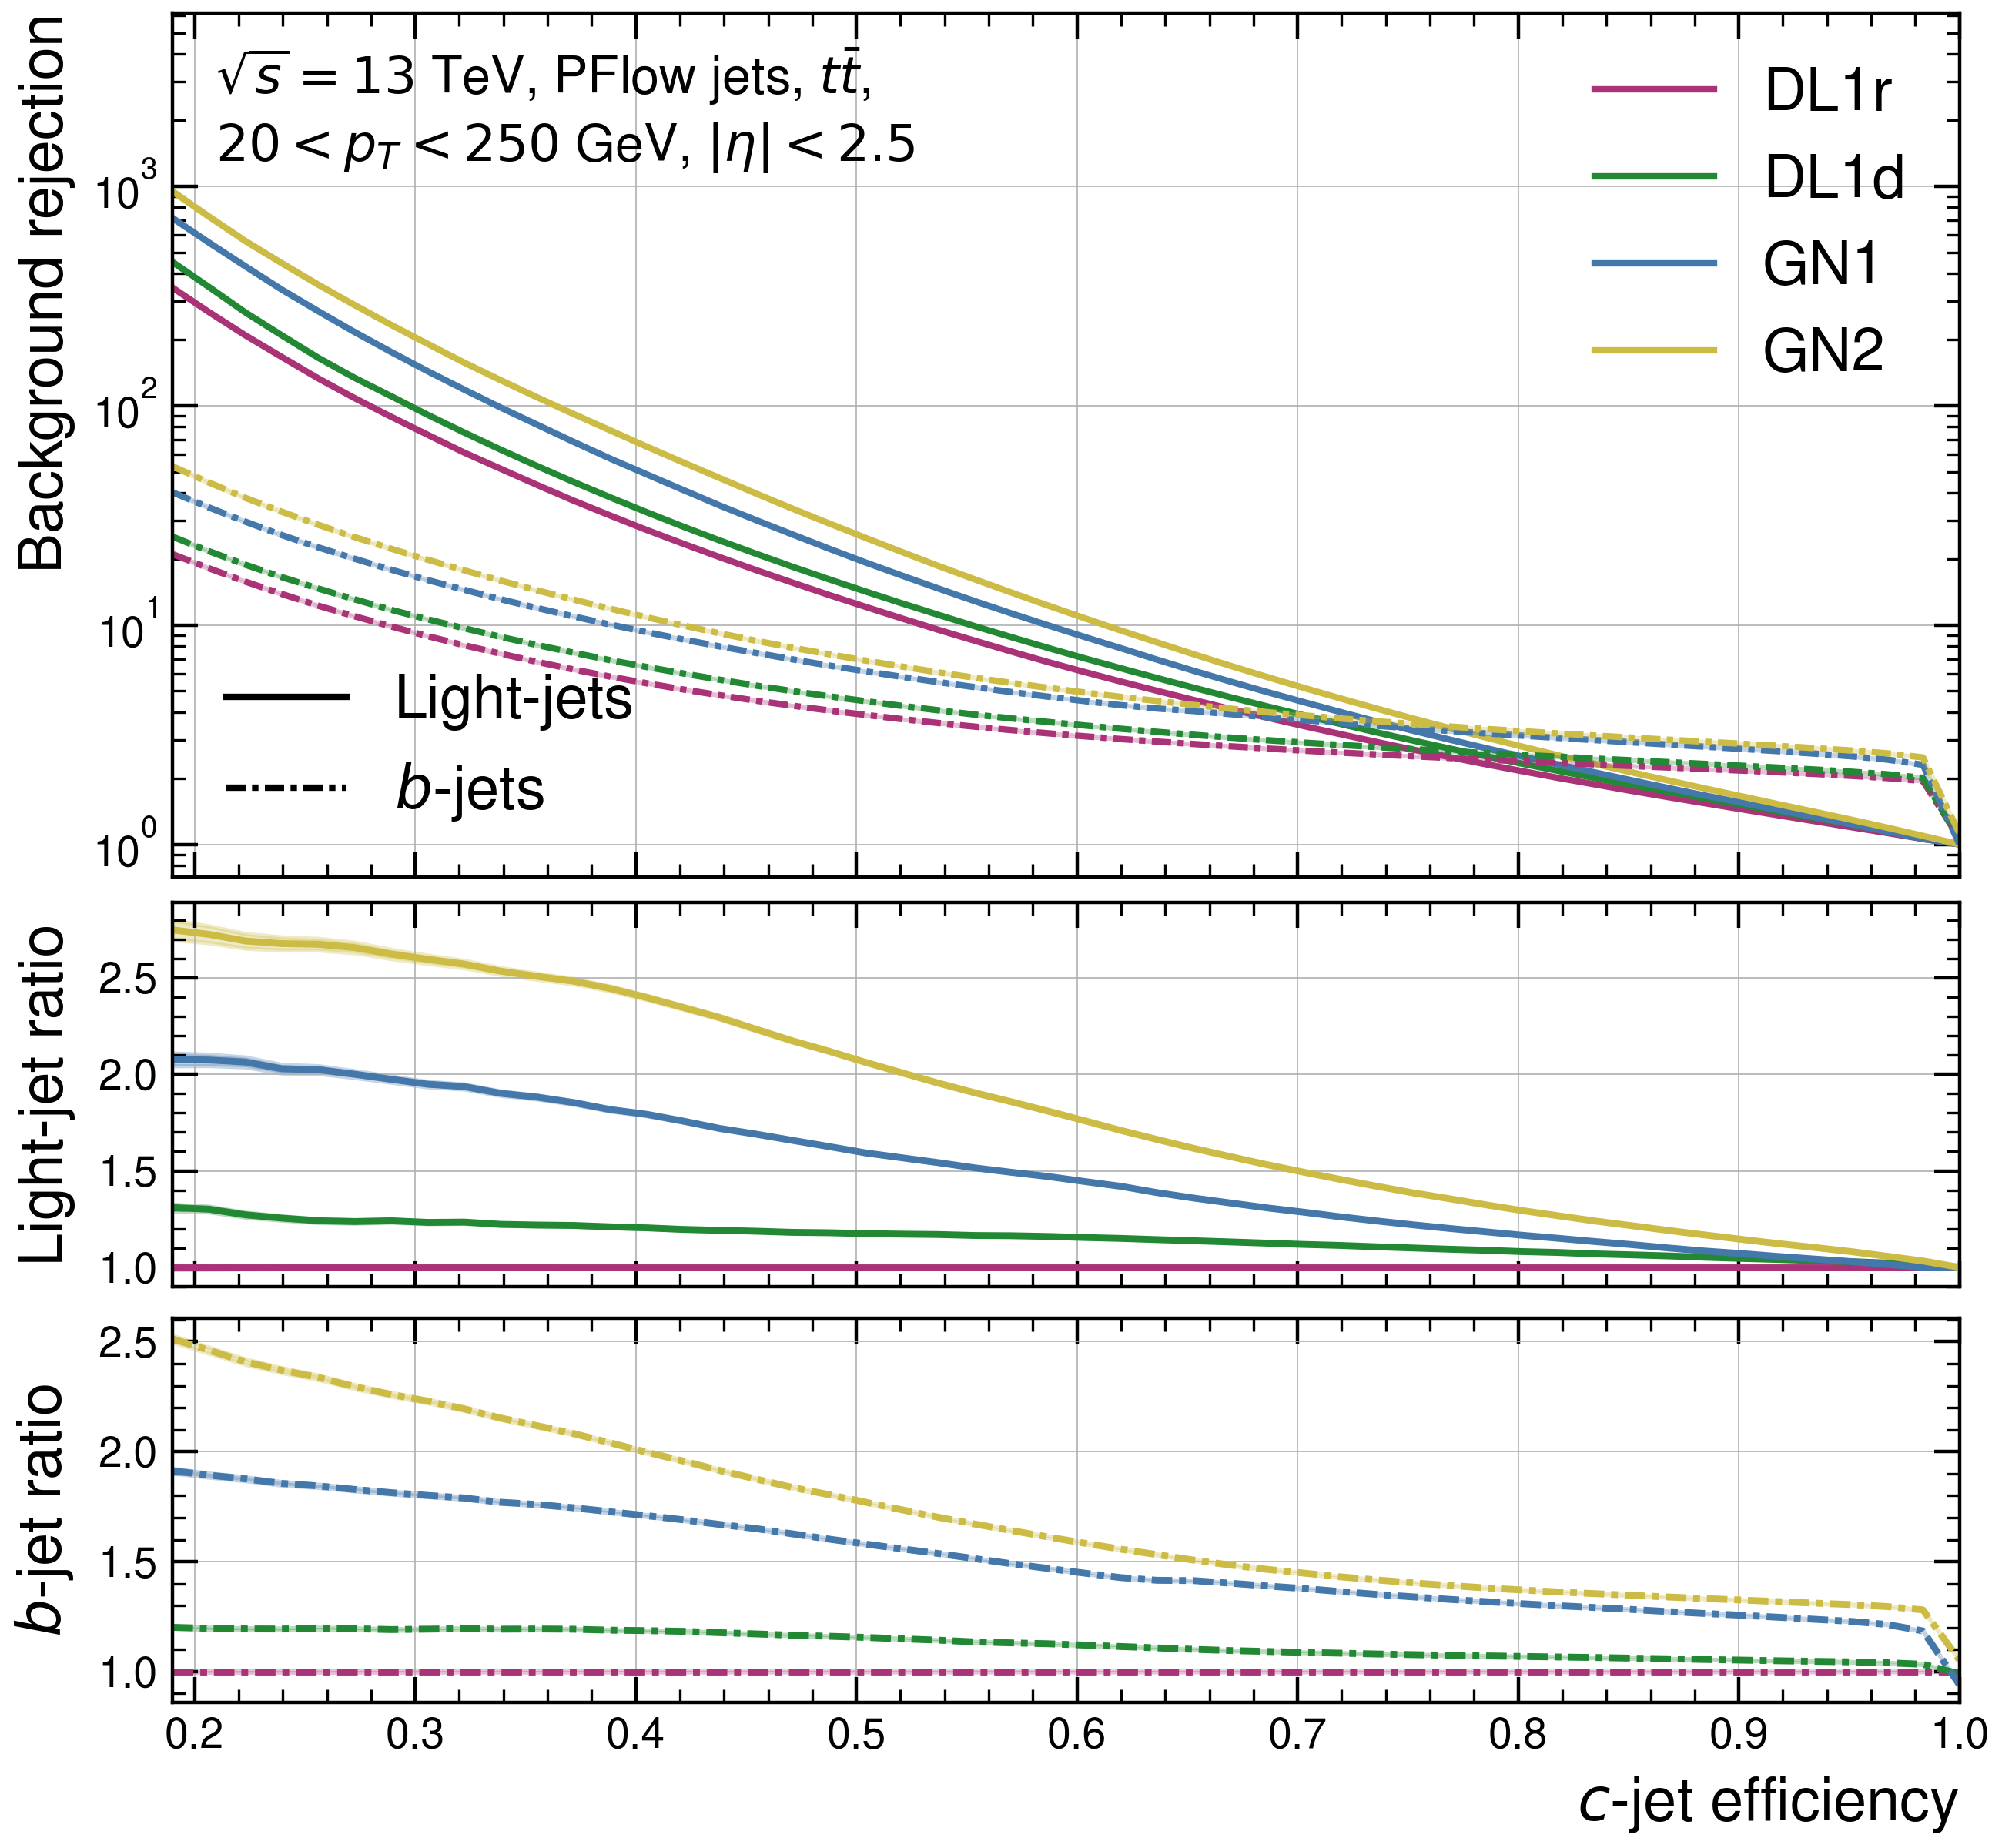
\includegraphics[width=0.50\textwidth]{Images/FTAG/GN/GN2/rocs/roc_ttbar_c.png}
  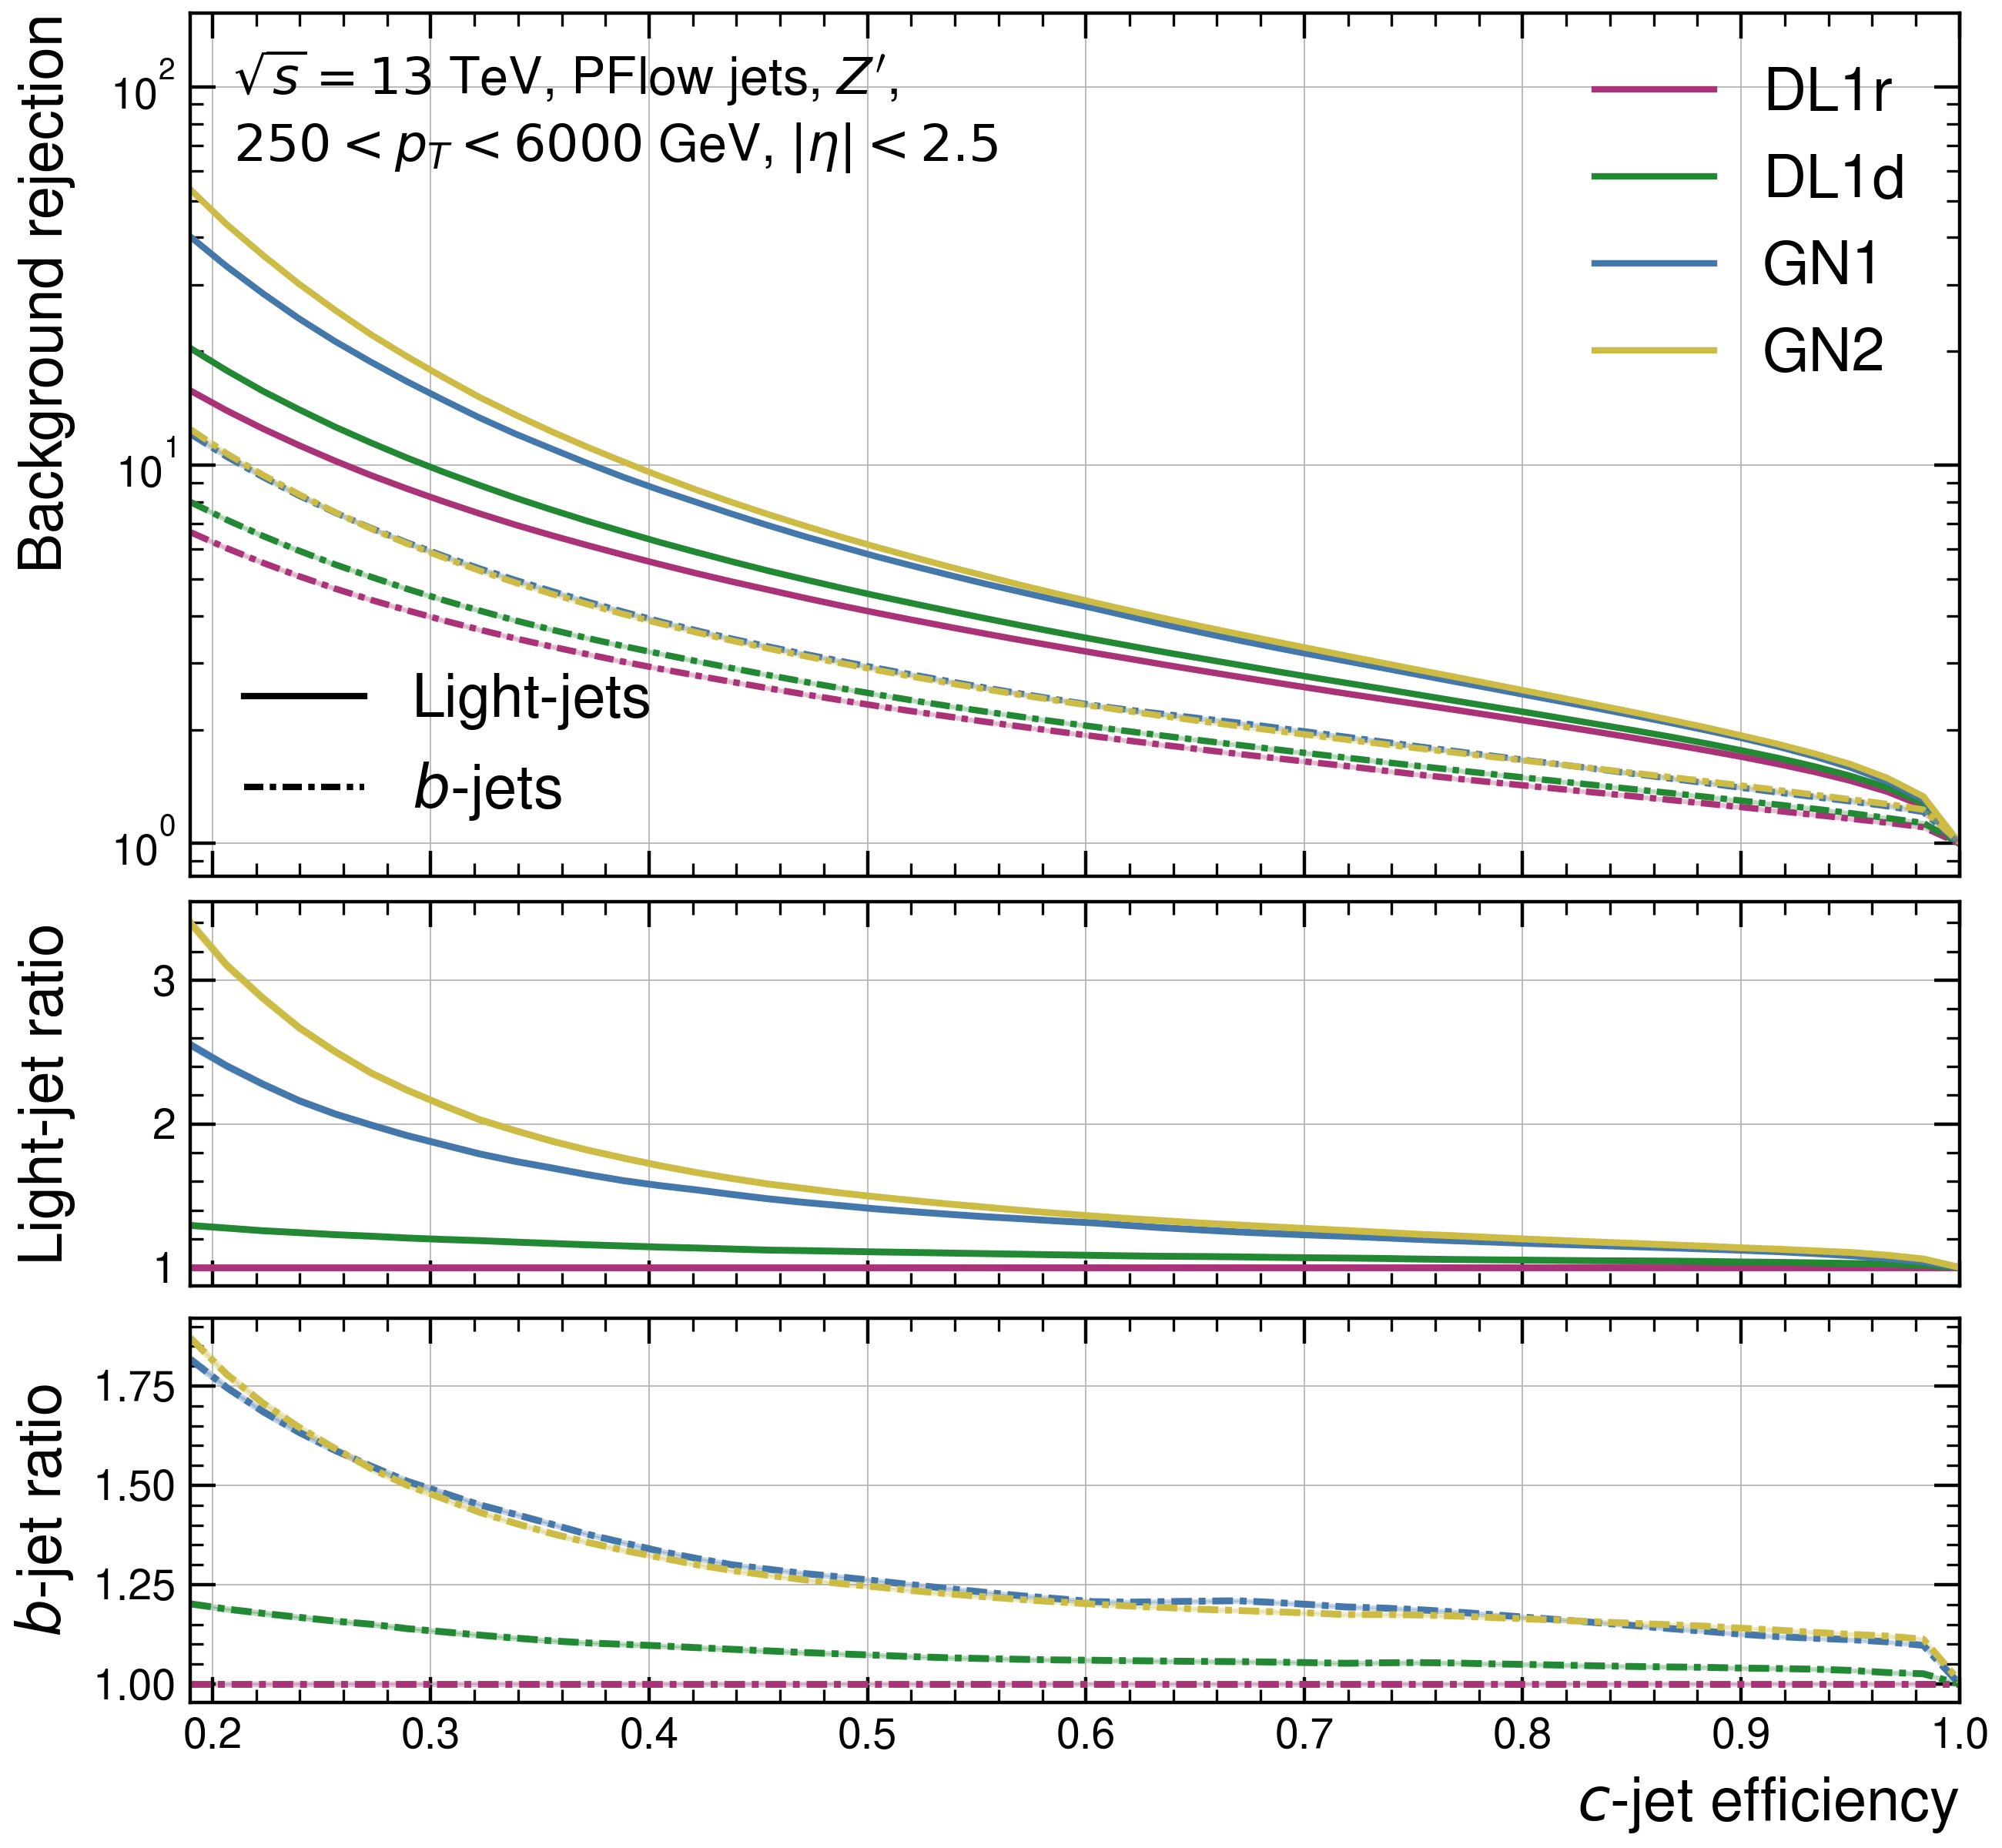
\includegraphics[width=0.50\textwidth]{Images/FTAG/GN/GN2/rocs/roc_zp_c.png}
  }
  \caption{The $b$- and light-rejections as a function of the $c$-jet tagging efficiency in the $t\bar{t}$ with $20 < p_T < 250$ GeV (left) and $Z'$ with $250 < p_T < 6000$ GeV (right) test samples. Models compared are DL1r in purple, DL1d in green, GN1 in blue, and GN2 in yellow. The bottom plots show the ratio to the DL1d performance. Flavour fractions are set at $f^c_b = 0.2$ for all models. Shaded regions represent the binominal error band.}
  \label{fig:GN2rocc}
  \end{figure}
\end{center}
 
Figure~\ref{fig:GNxscansfb} displays the flavour fraction $f^c_b$ scans for $c$-tagging at the 30\% \gls{wp}. The same conclusions as for $b$-tagging hold, underlying the overall superiority of \gls{gn2}. The $f_b^c$ scans for $c$-tagging show a different shape than the $b$-tagging ones: at large $f^b_c$, the $b$-rejection rapidly increases while for $b$-tagging the $c$-rejection is saturating. This behaviour is due to the comparatively easier identification of $b$-jets compared to the overlap of $c$- and light-jets. \\

\begin{figure}[h!]
  \centering
  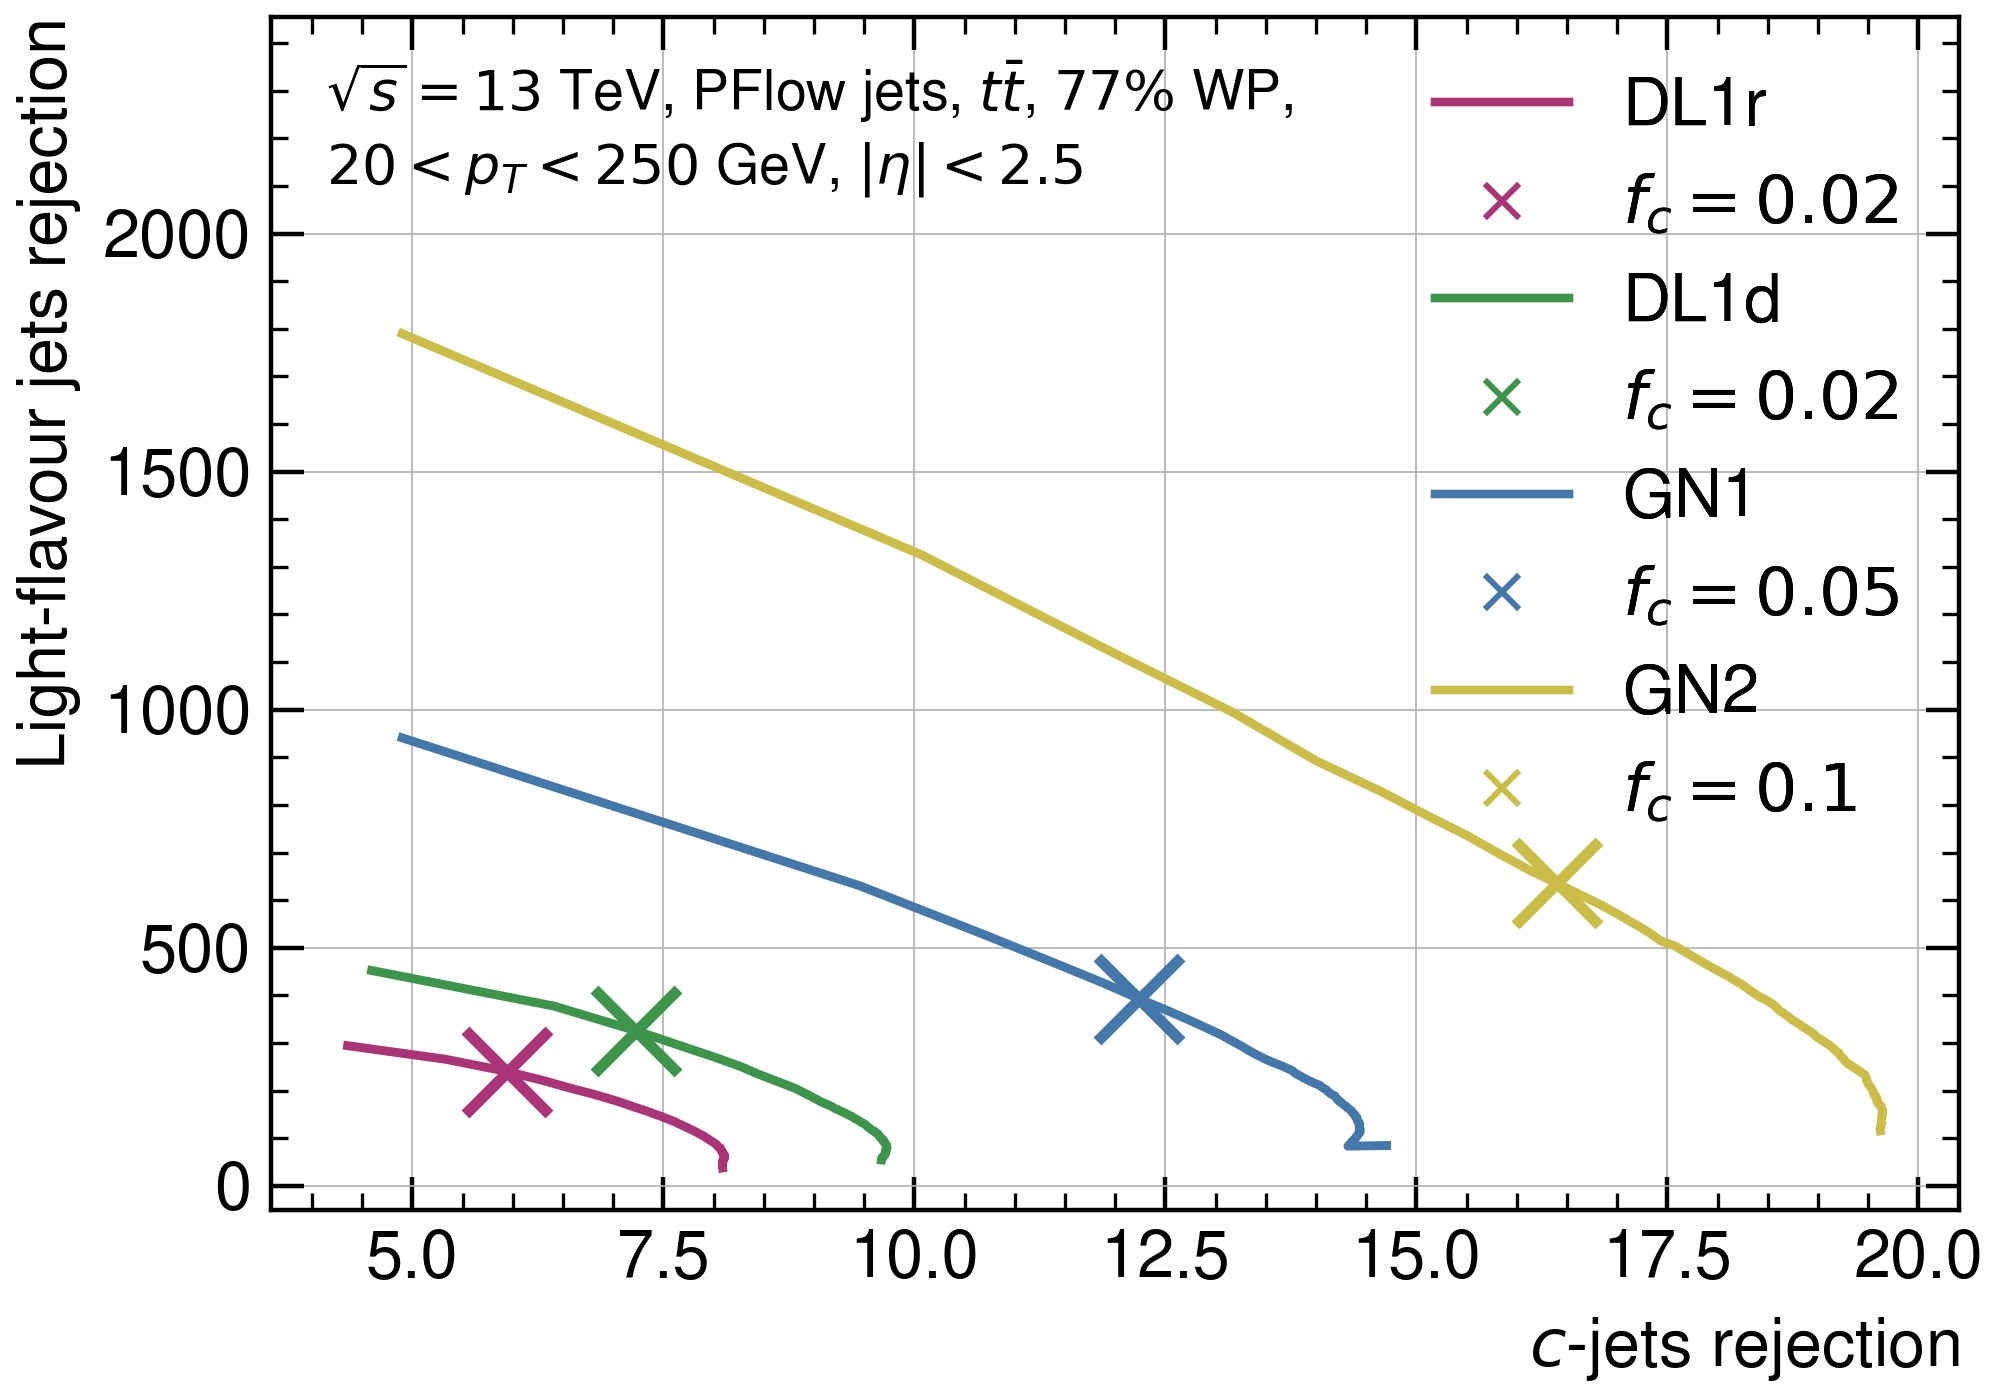
\includegraphics[width=0.48\textwidth]{Images/FTAG/GN/GN2/fraction_scans/FractionScanPlot_tt.png}
  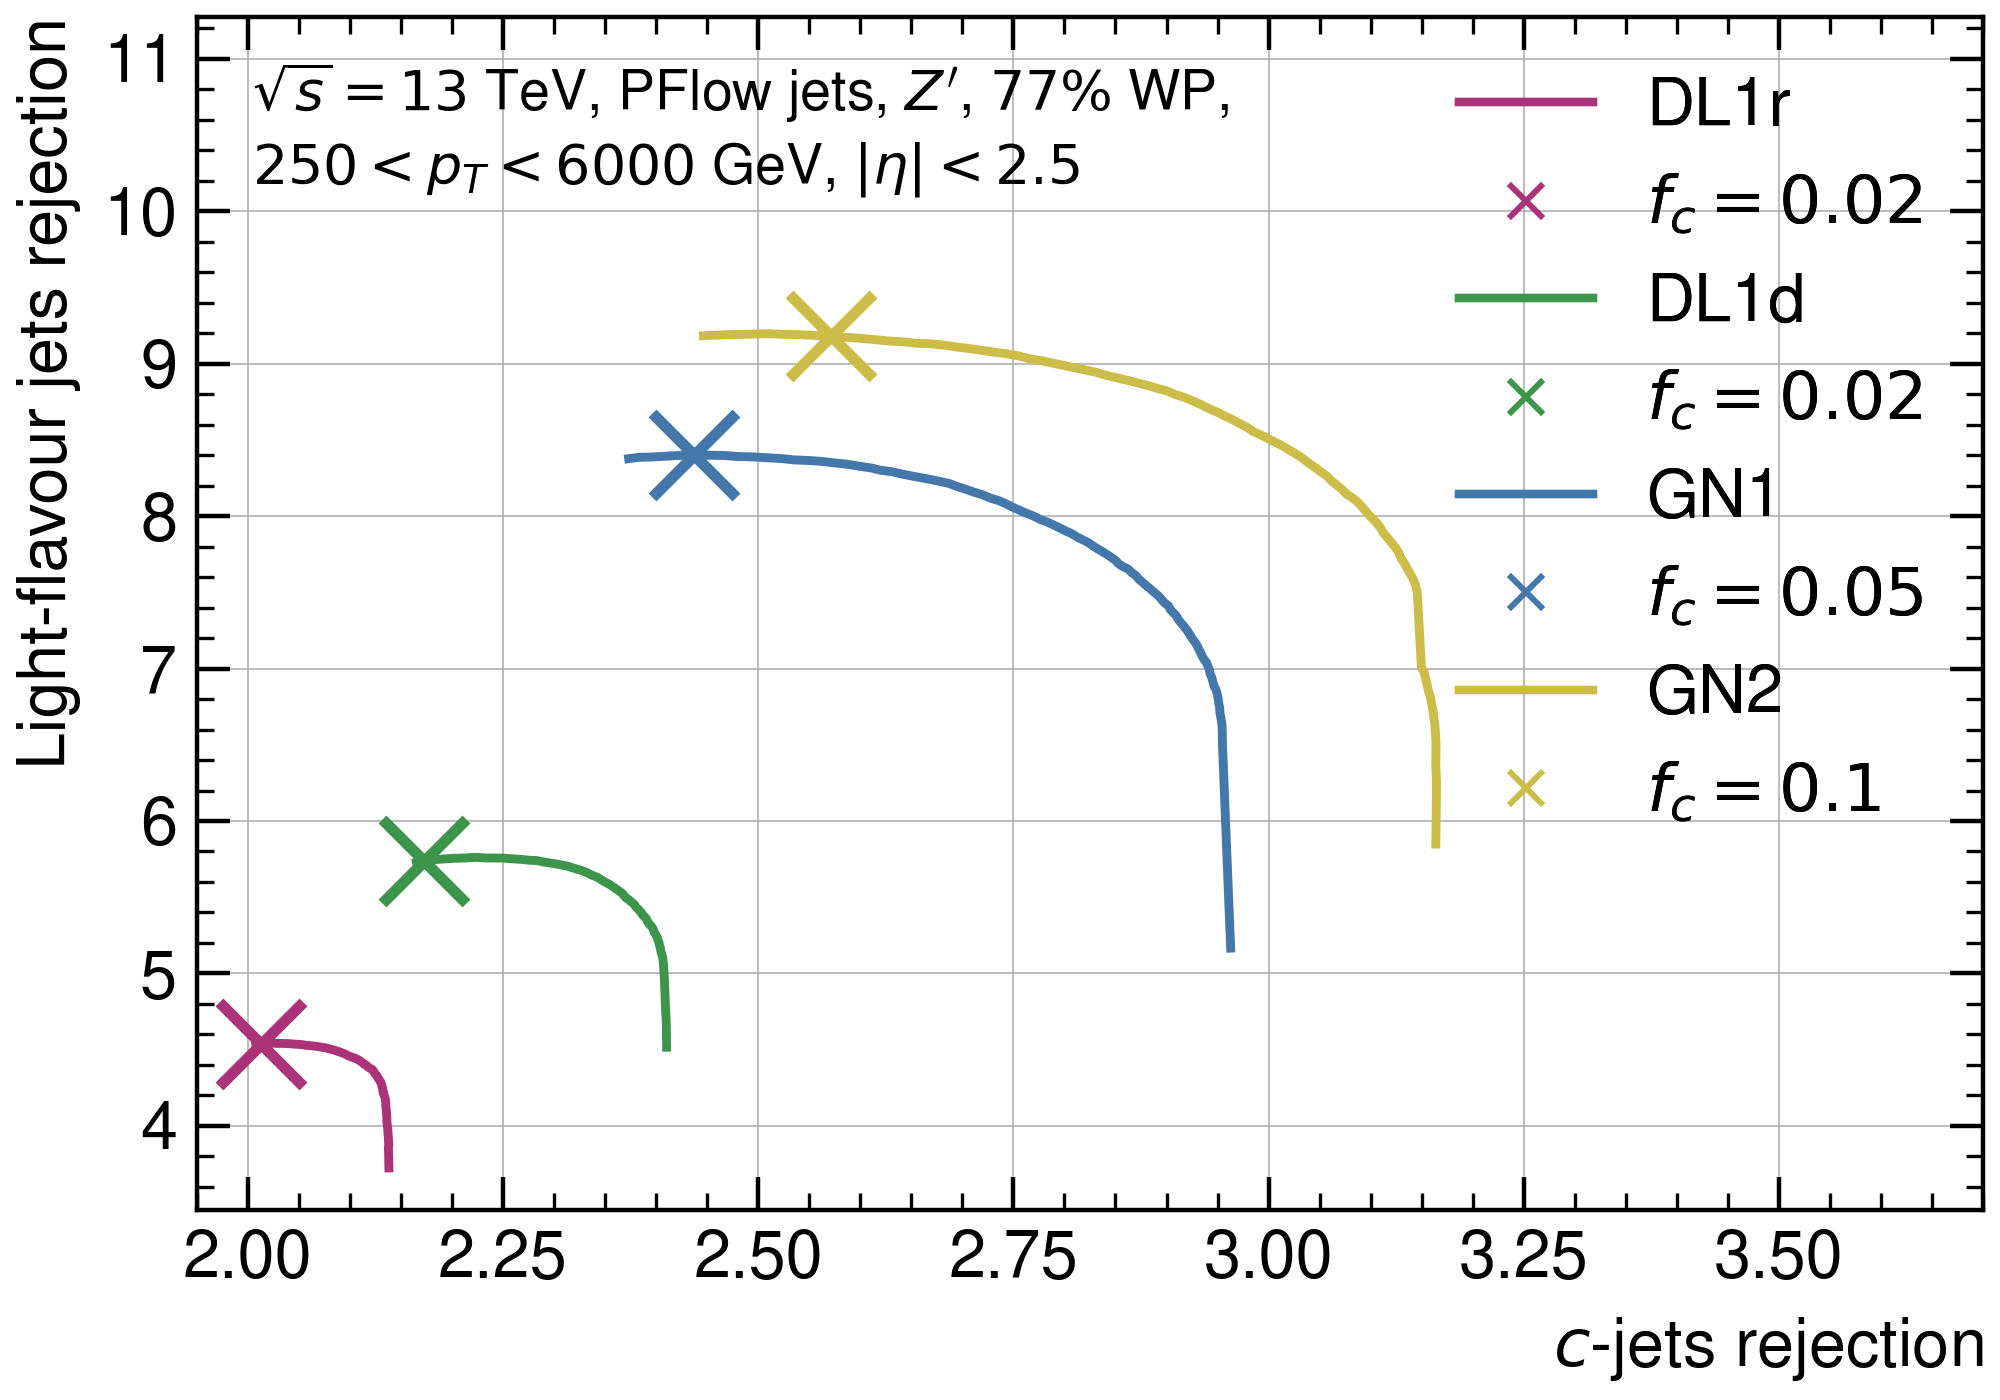
\includegraphics[width=0.48\textwidth]{Images/FTAG/GN/GN2/fraction_scans/FractionScanPlot_zp.png}
  \caption{The flavour fraction $f^b_c$ scans for $b$-tagging at a fixed \gls{wp} of 77\% of the different models considered evaluated on the $t\bar{t}$ (left) and $Z'$ (right). The chosen values are marked on the curves, displaying on the $x$-axis the $c$-rejection vs the light-rejection on the $y$ axis. Increasing $f^b_c$ shifts the marker rightwards along the curves. }
  \label{fig:GNxscansfc}
\end{figure}

\begin{figure}[h!]
  \centering
  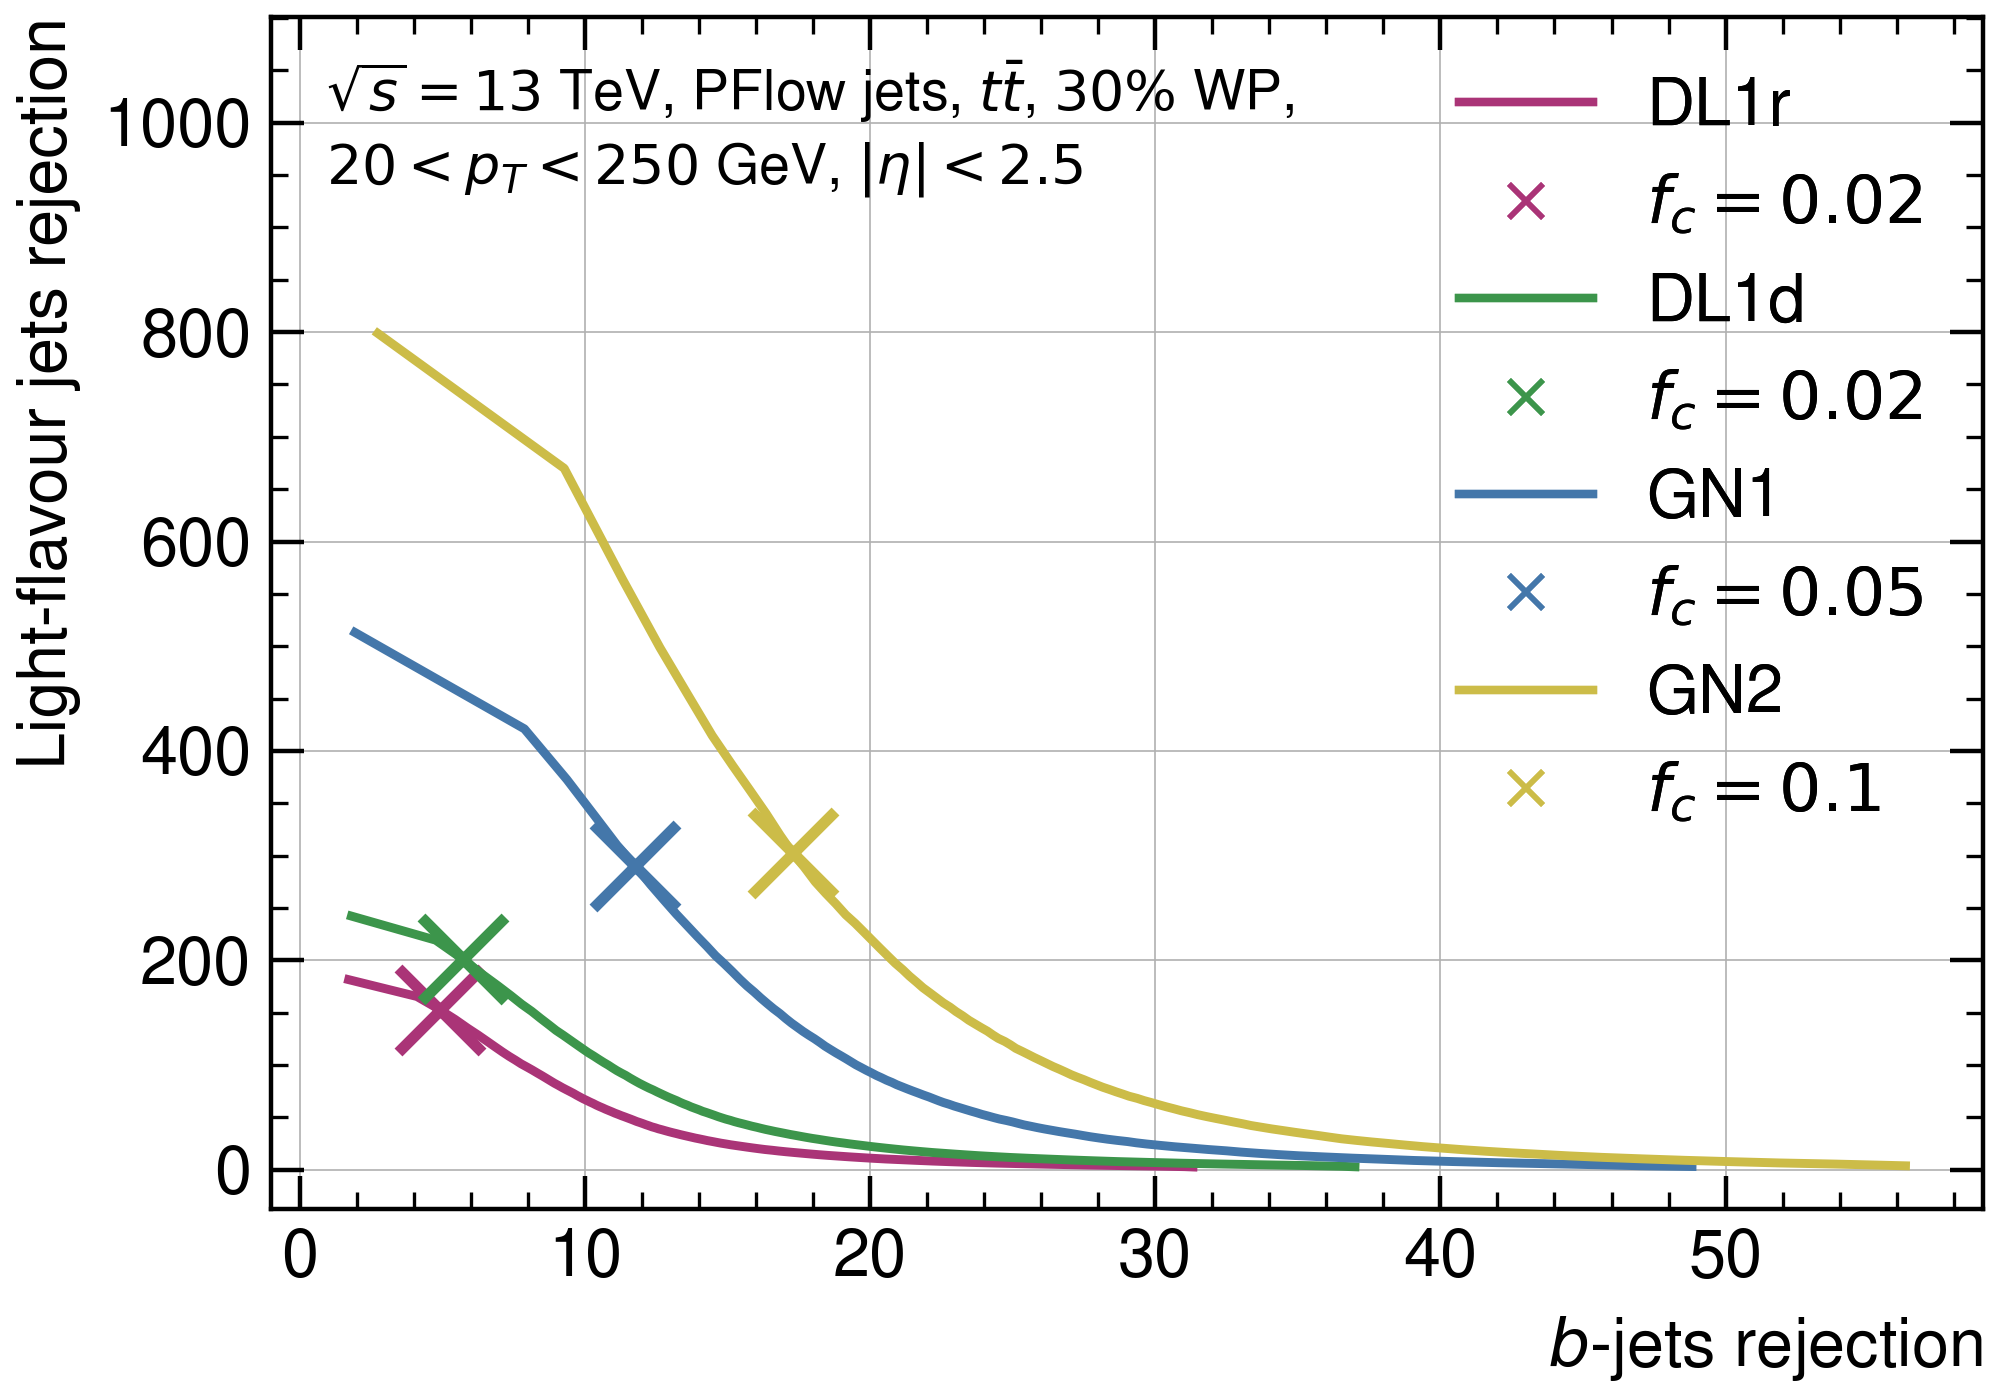
\includegraphics[width=0.48\textwidth]{Images/FTAG/GN/GN2/fraction_scans/FractionScanPlot_tt_c.png}
  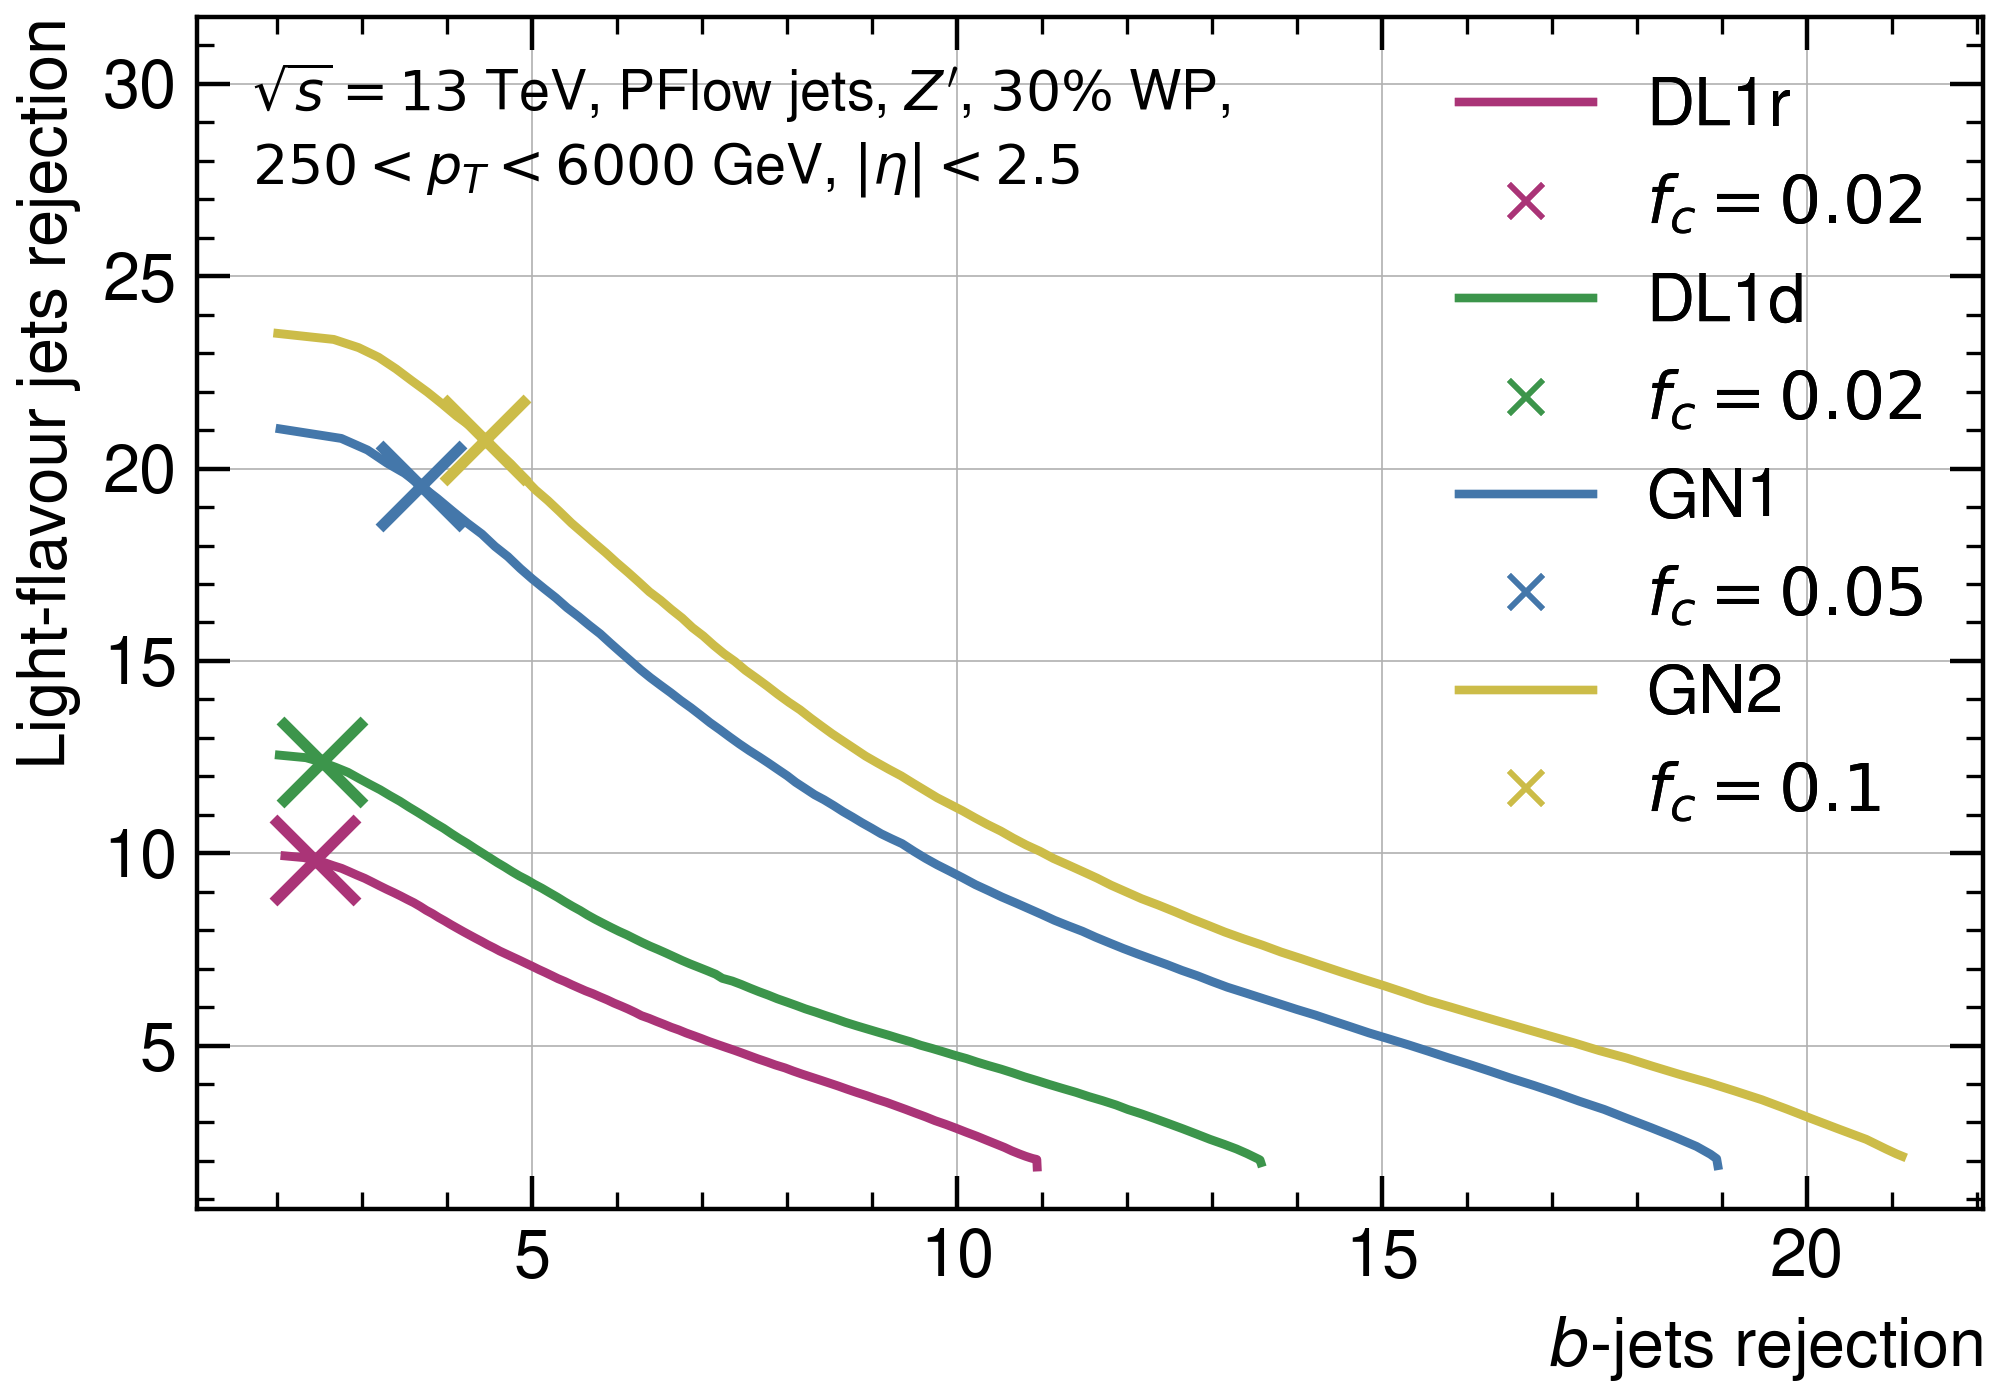
\includegraphics[width=0.48\textwidth]{Images/FTAG/GN/GN2/fraction_scans/FractionScanPlot_zp_c.png}
  \caption{The flavour fraction $f^c_b$ scans for $c$-tagging at a fixed \gls{wp} of 30\% of the different models considered evaluated on the $t\bar{t}$ (left) and $Z'$ (right). The chosen values are marked on the curves, displaying on the $x$-axis the $b$-rejection vs the light-rejection on the $y$ axis. Increasing $f^c_b$ shifts the marker rightwards along the curves. }
  \label{fig:GNxscansfb}
\end{figure} 

% Eff for fixed WP
Figure~\ref{fig:GNxptb_eff} displays the effective per-bin $b$-tagging efficiency for an inclusive $b$-tagging efficiency of 70\% for $t\bar{t}$ and 30\% for $Z'$ in each $p_T$ region considered. The performance is not uniform across $p_T$, with the model better accommodating specific parts of the $p_T$ spectrum. The region [100, 800] GeV overlapping the two samples is a sweet spot for performance, with more challenging results at lower and higher $p_T$. The performance for $Z'$ in particular reduces dramatically with larger momentum, due to the physics reasons previously explained. Figure~\ref{apfig:GNxptc_eff} in Appendix \ref{app-GN2sup} displays the same information for $c$-tagging, leading to the same conclusions. \\
\begin{figure}[h!]
  \centering
  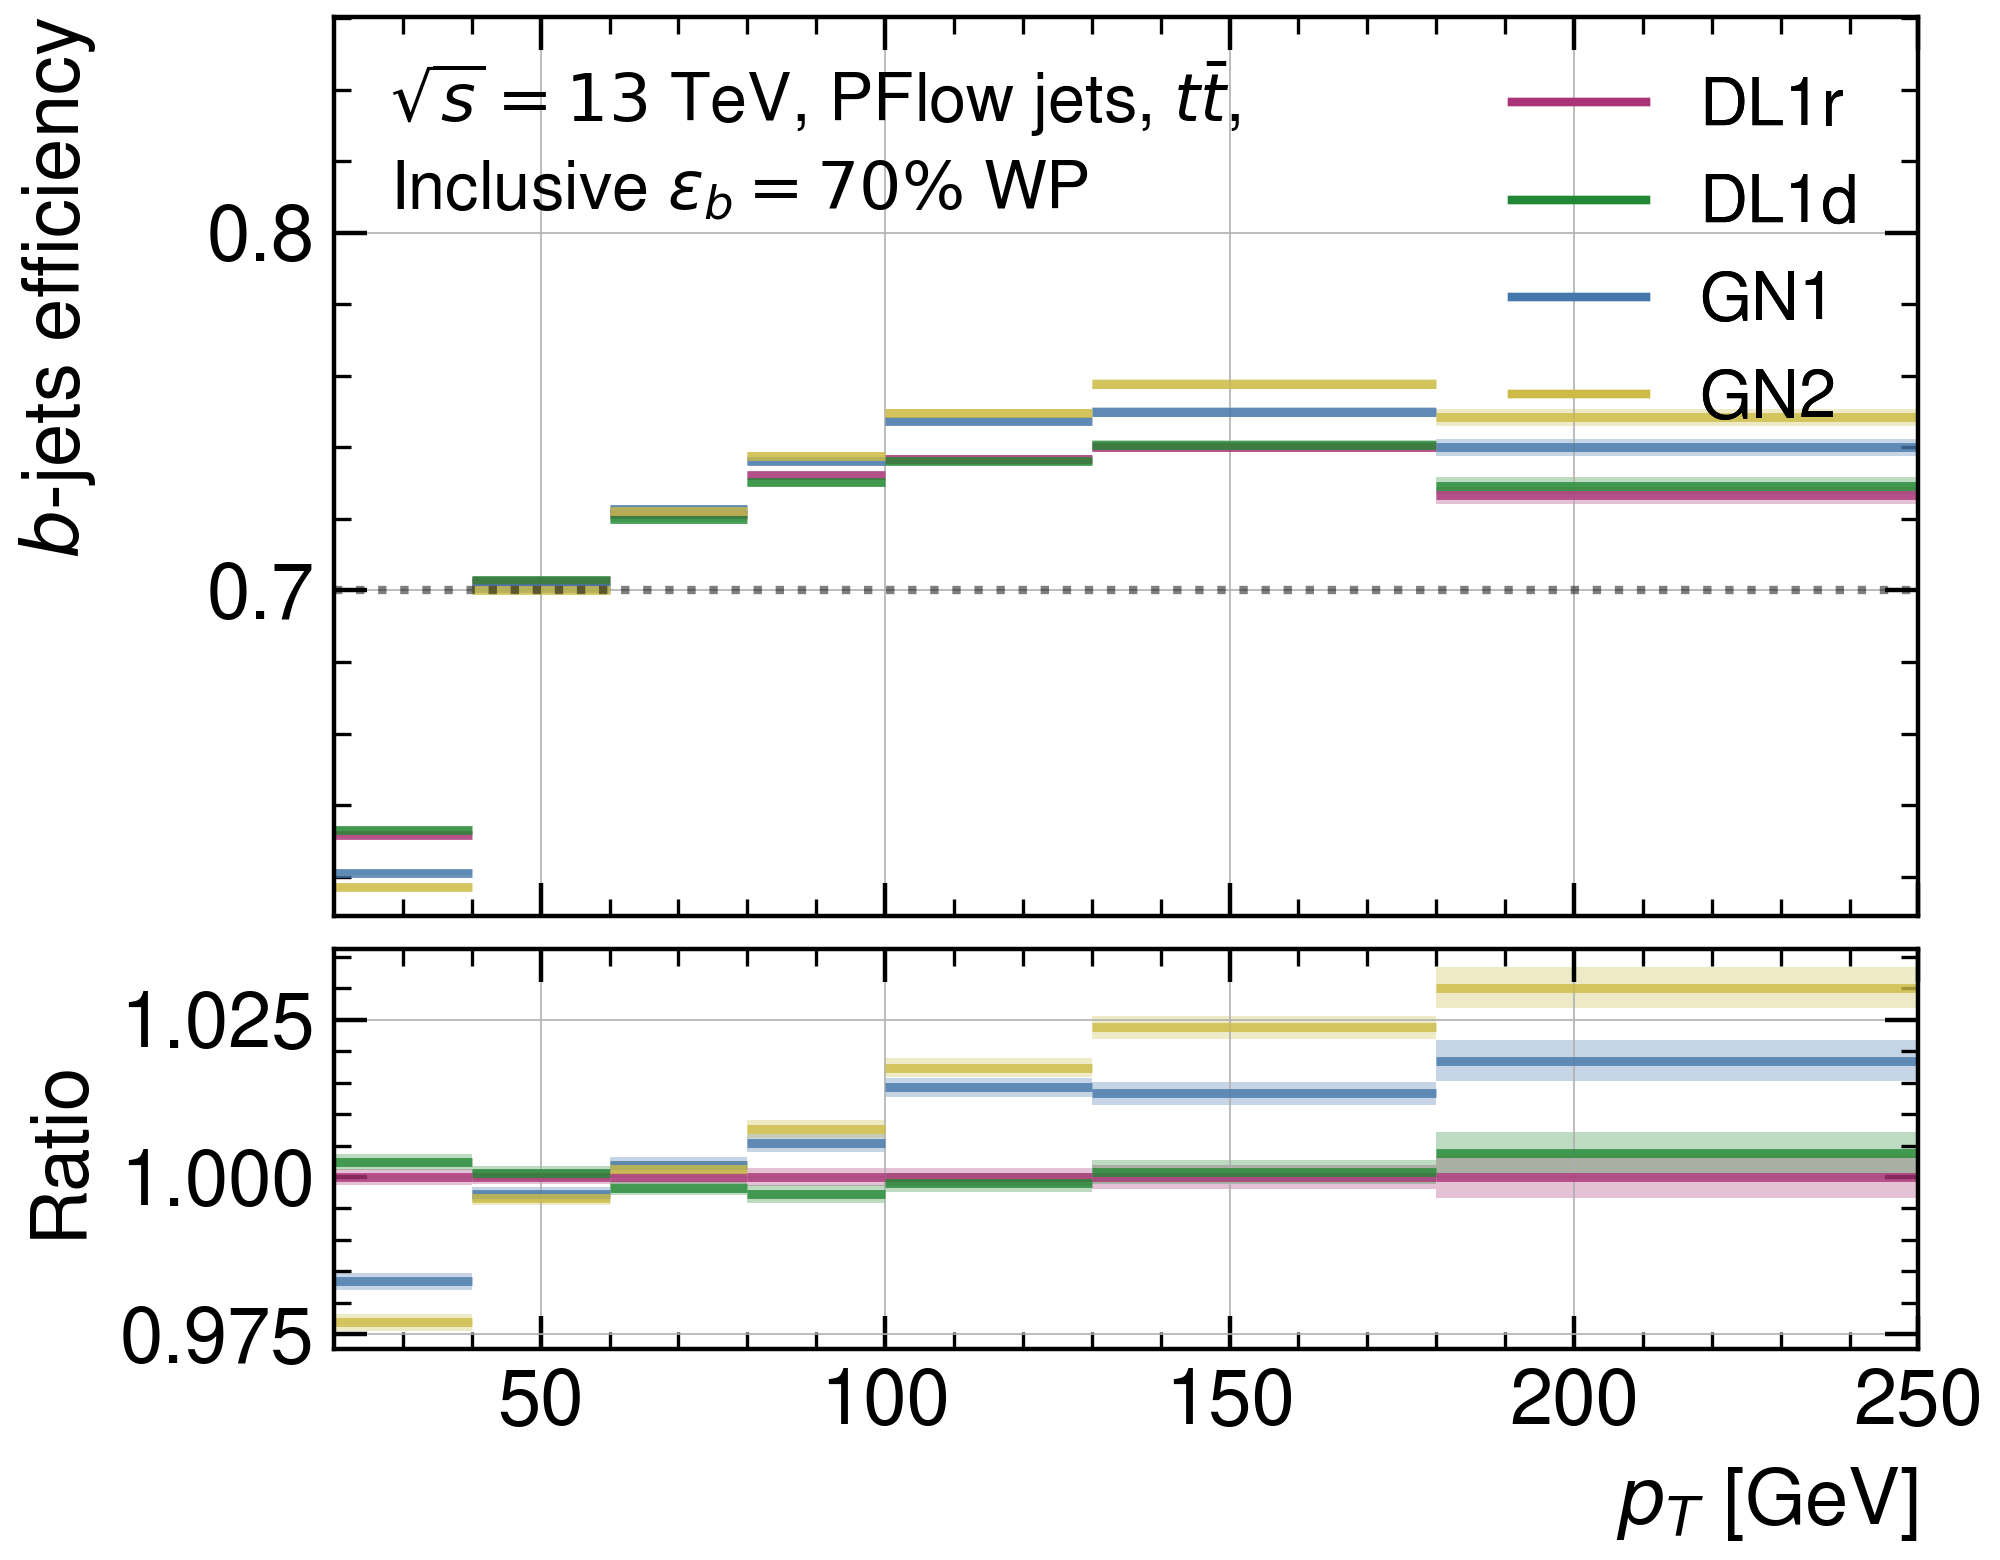
\includegraphics[width=0.48\textwidth]{Images/FTAG/GN/GN2/pt_plots/pt_ttbar_b_eff.png}
  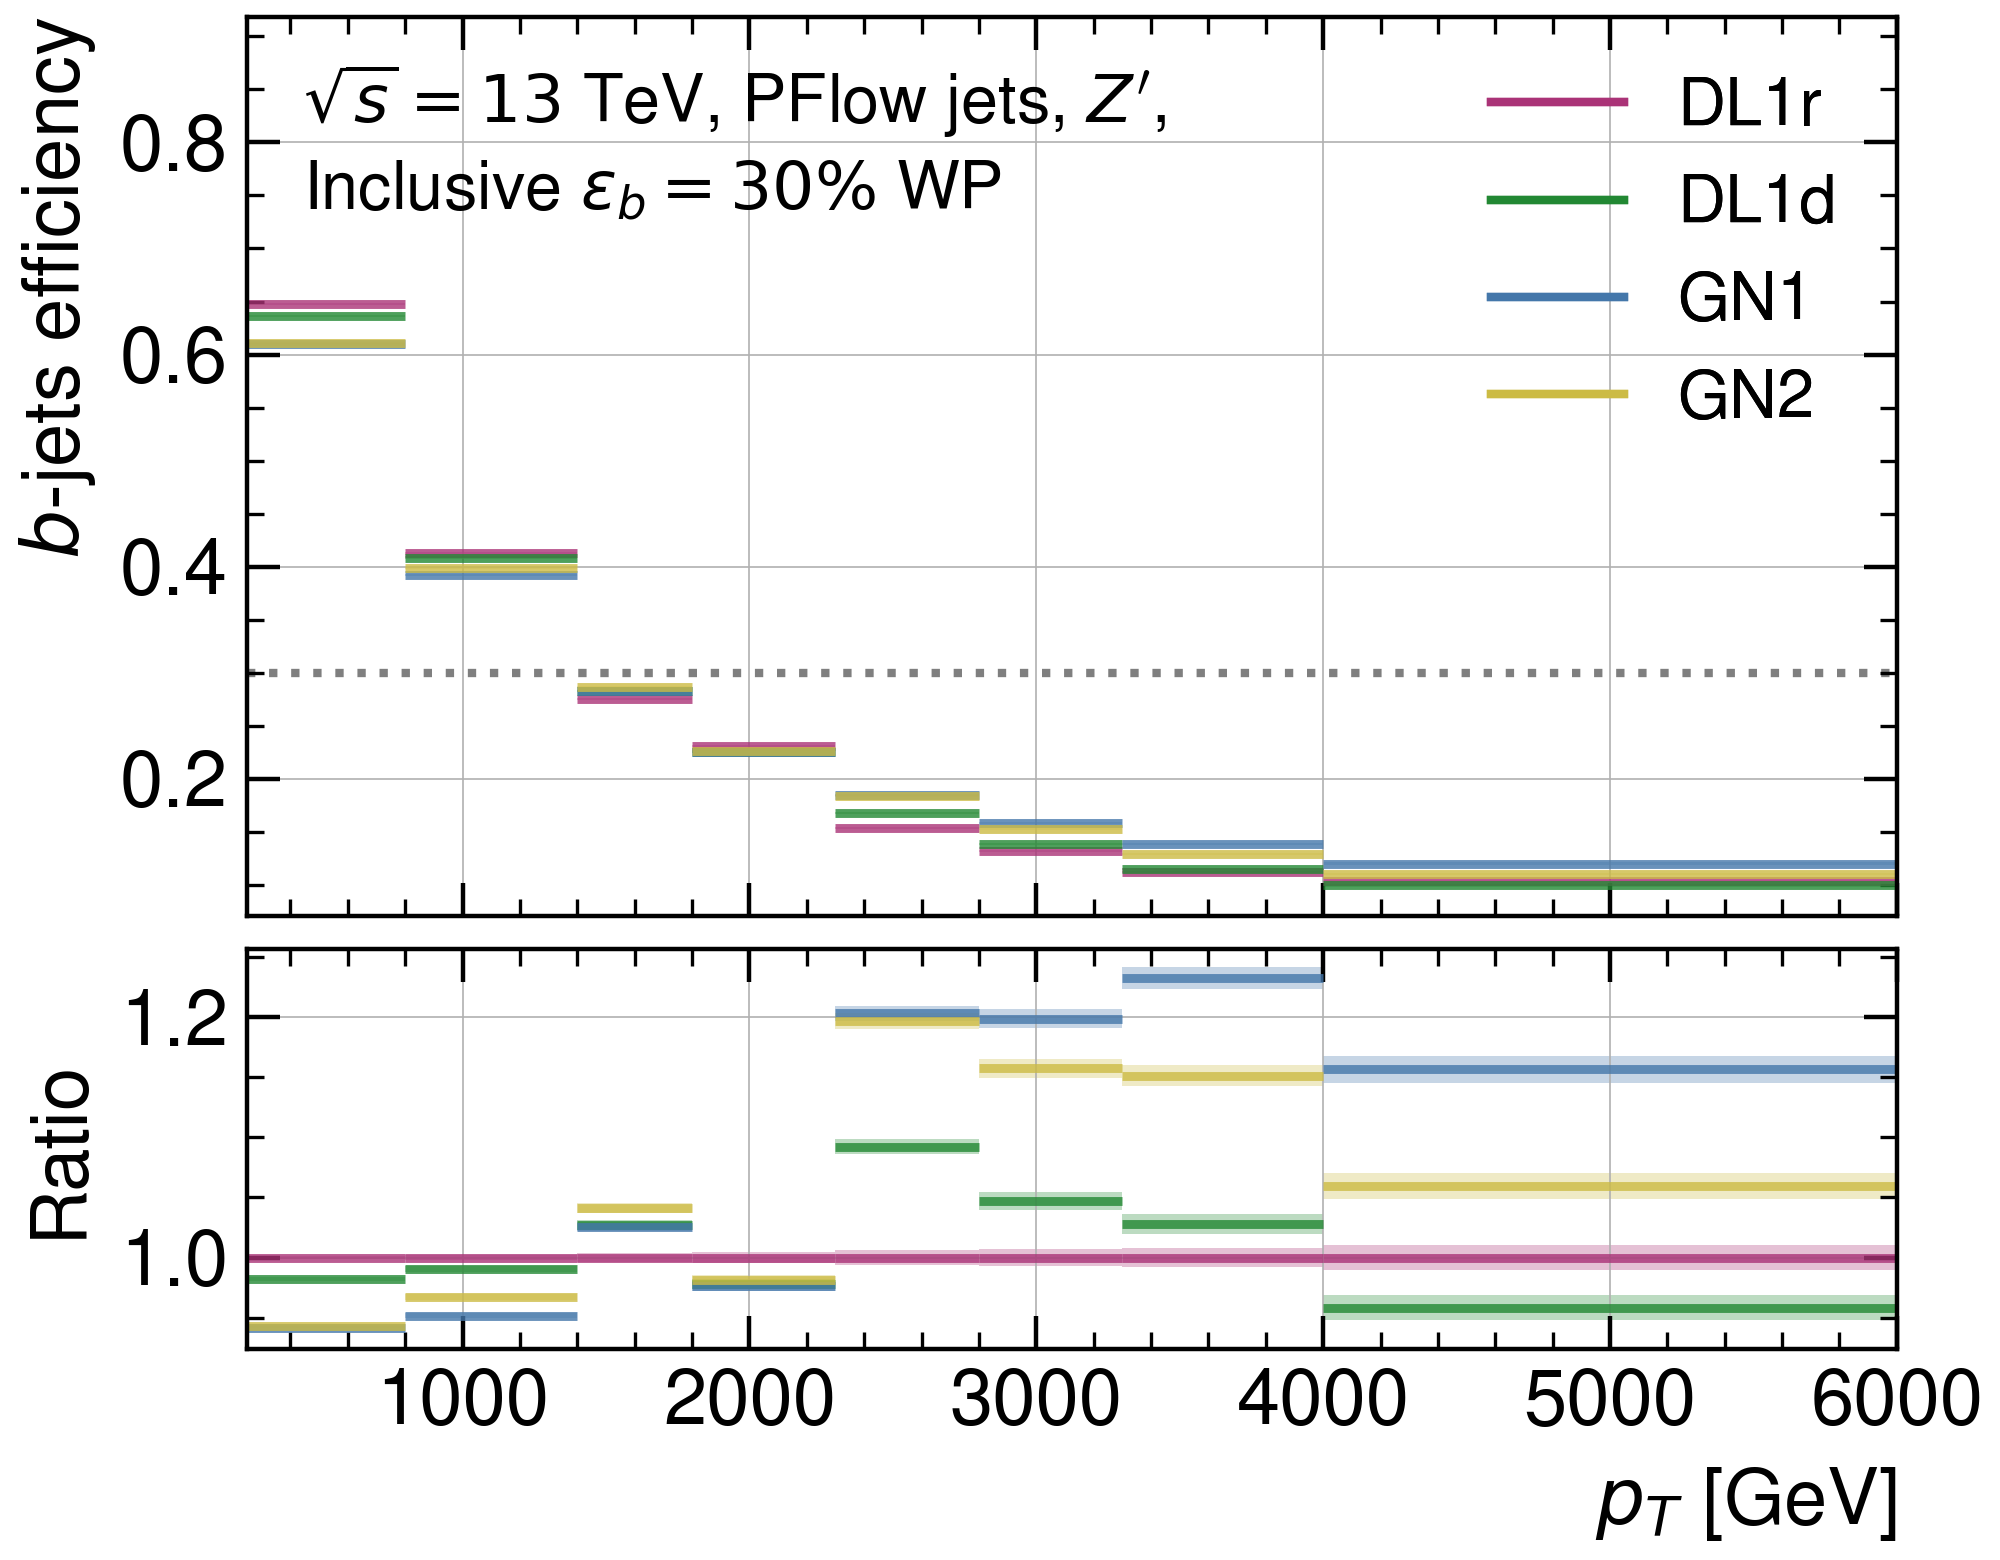
\includegraphics[width=0.48\textwidth]{Images/FTAG/GN/GN2/pt_plots/pt_zp_b_eff.png}
  \caption{Comparing the different models $b$-tagging efficiency as a function of jet $p_T$ for the inclusive $b$-tagging 70\% \gls{wp} on the $t\bar{t}$ (left) and 30\% \gls{wp} on $Z'$ (right). The flavour fraction is set at $f^b_c = 0.018$ for DL1r and DL1d, 0.05 for GN1, and 0.1 for GN2.}
  \label{fig:GNxptb_eff}
\end{figure} 
% Eff fixed light
\begin{figure}[h!]
  \centering
  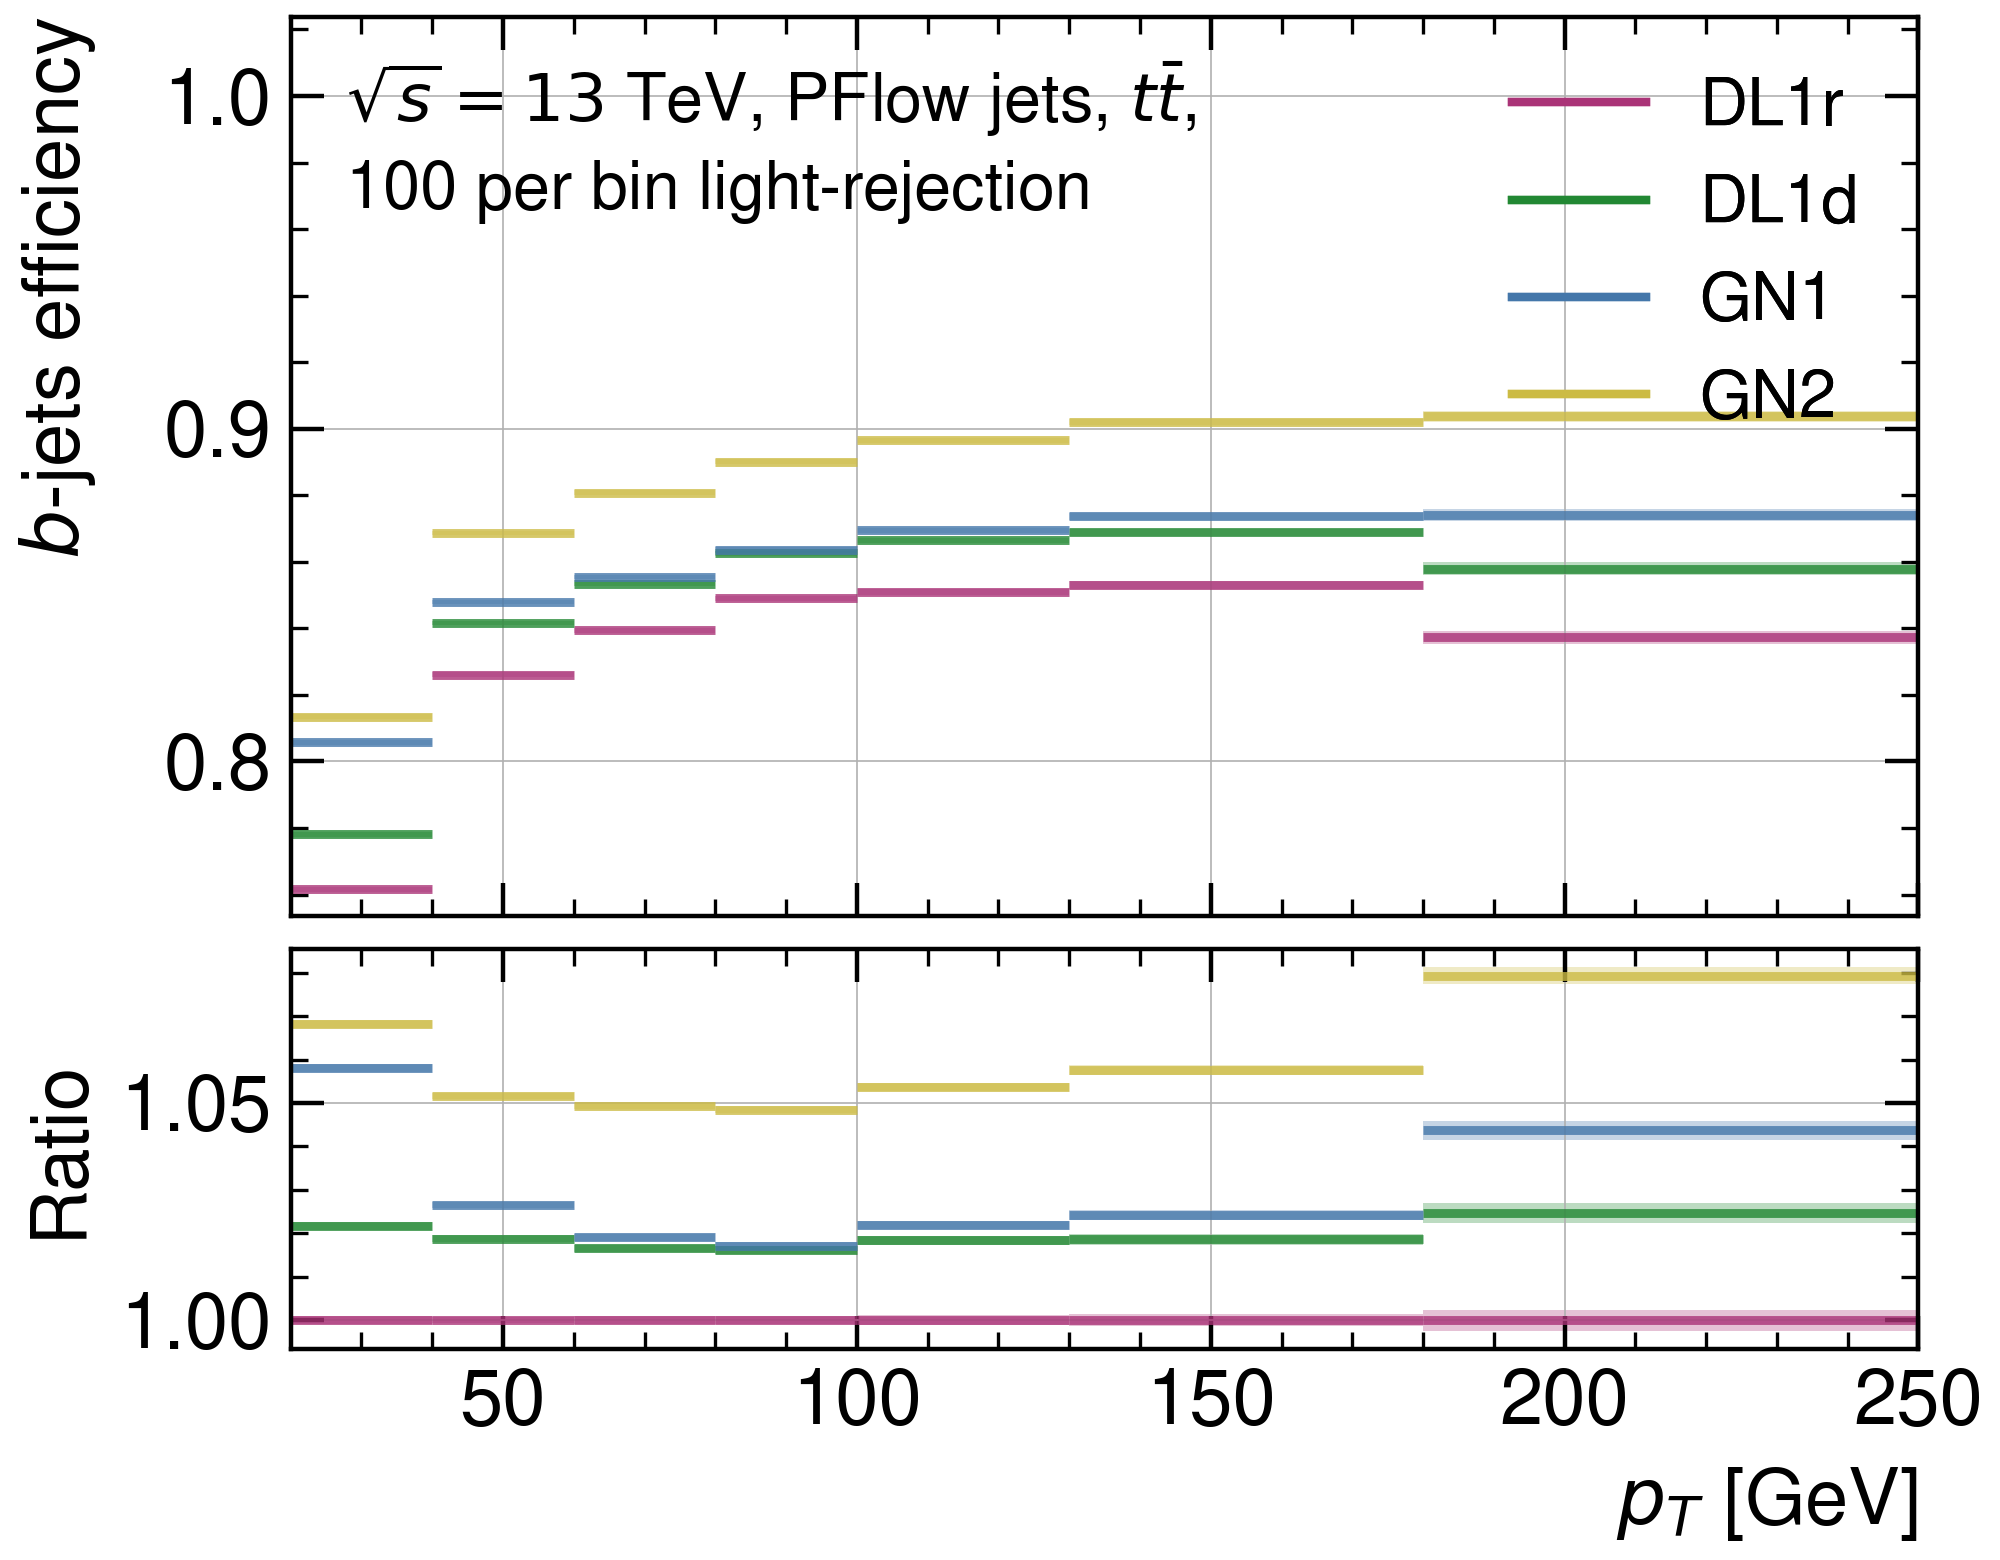
\includegraphics[width=0.48\textwidth]{Images/FTAG/GN/GN2/pt_plots/pt_ttbar_b_eff_fixedlight.png}
  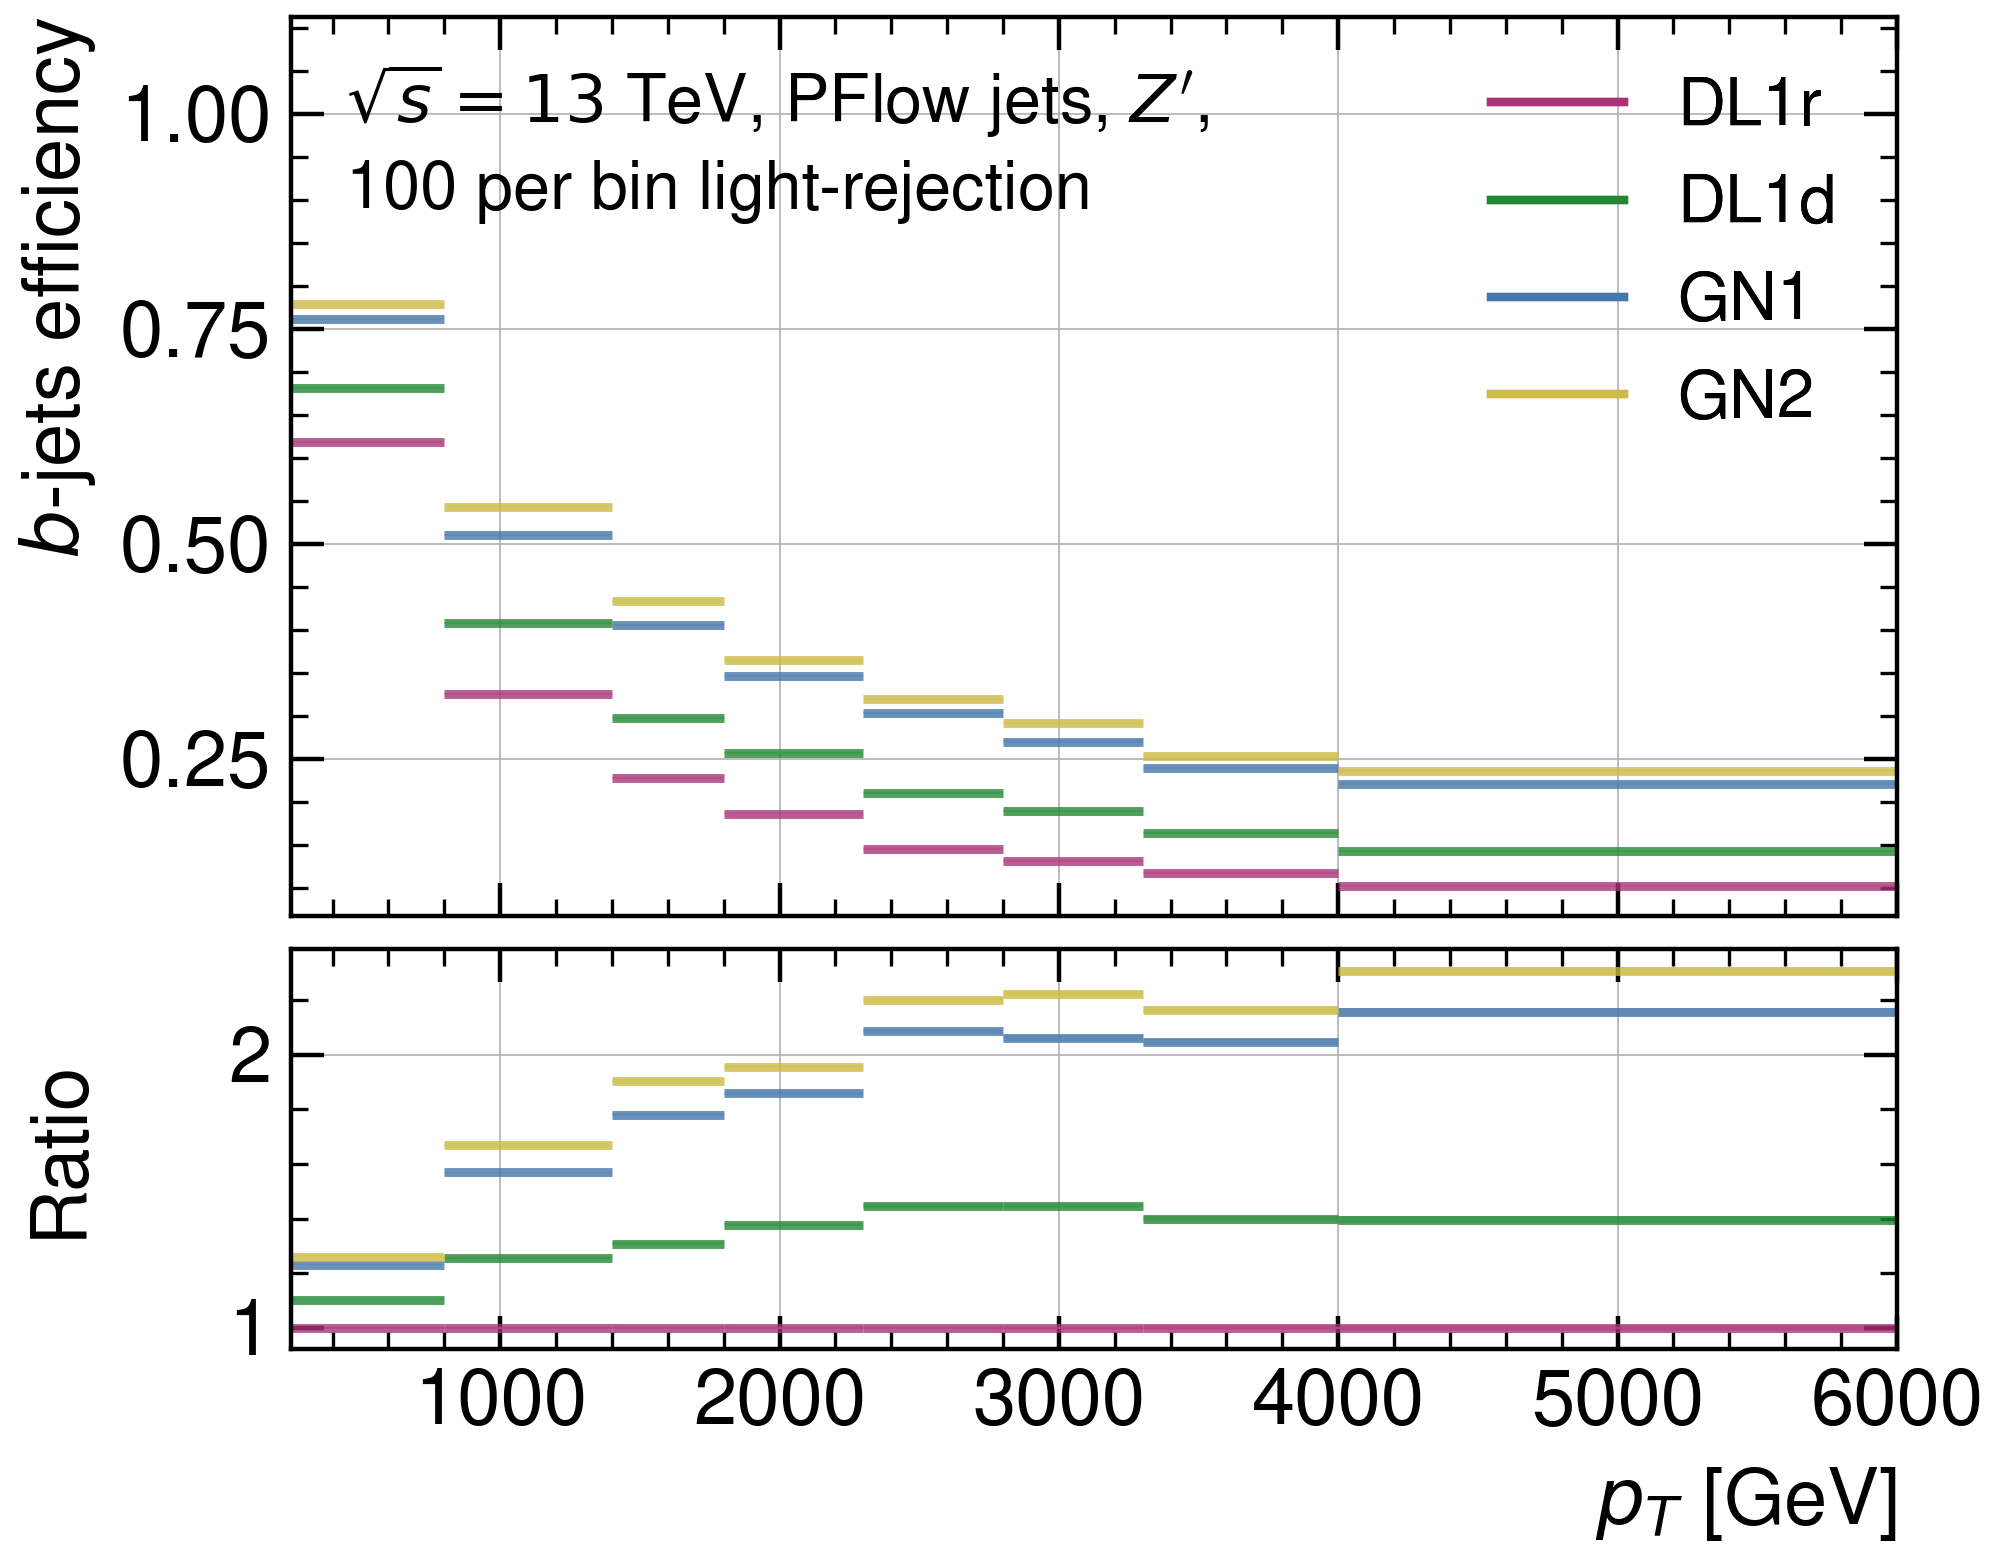
\includegraphics[width=0.48\textwidth]{Images/FTAG/GN/GN2/pt_plots/pt_zp_b_eff_fixedlight.png}
  \caption{Comparing the different models $b$-tagging efficiency as a function of jet $p_T$ at a fixed 100 light-jet rejection per bin on the $t\bar{t}$ (left) and $Z'$ (right) test samples. The flavour fraction is set at $f^b_c = 0.018$ for DL1r and DL1d, 0.05 for GN1, and 0.1 for GN2.}
  \label{fig:GNxptb_efffixedl}
\end{figure} 

To avoid biasing the analysis of the results with this per-bin performance dependency, Figure~\ref{fig:GNxptb_efffixedl} displays the $b$-tagging efficiency distribution across $p_T$ at a fixed per-bin light-rejection of 100. The superior capabilities of \gls{gn2} are exhibited across the $p_T$ spectrum. The same conclusion holds for $c$-tagging, as displayed in Figure~\ref{apfig:GNxptc_efffixedl} of the appendix. Inspecting the rejections at a fixed $b$-tagging efficiency of 70\% per bin also leads to concluding the clear superiority of \gls{gn2}. Figures \ref{fig:GNxptb_crejflat} and \ref{fig:GNxptb_urejflat} respectively display the $c$- and light-rejection for a 70\% per-bin $b$-efficiency, showing that most of the improvement from \gls{gn2} and \gls{gn1} is in the [100, 800] GeV $p_T$ region. The same distribution with an inclusive 70\% $b$-tagging efficiency, over the entire $p_T$ regions, is displayed in Figures \ref{apfig:GNxptb_crej} and \ref{apfig:GNxptb_urej} of the appendix. The $b$- and light-rejection at the 30\% $c$-tagging per-bin \gls{wp} are displayed in Figures \ref{fig:GNxptc_brejflat} and \ref{fig:GNxptc_urejflat} respectively. \\

% Rej c - flat btagging
\begin{figure}[h!]
  \centering
  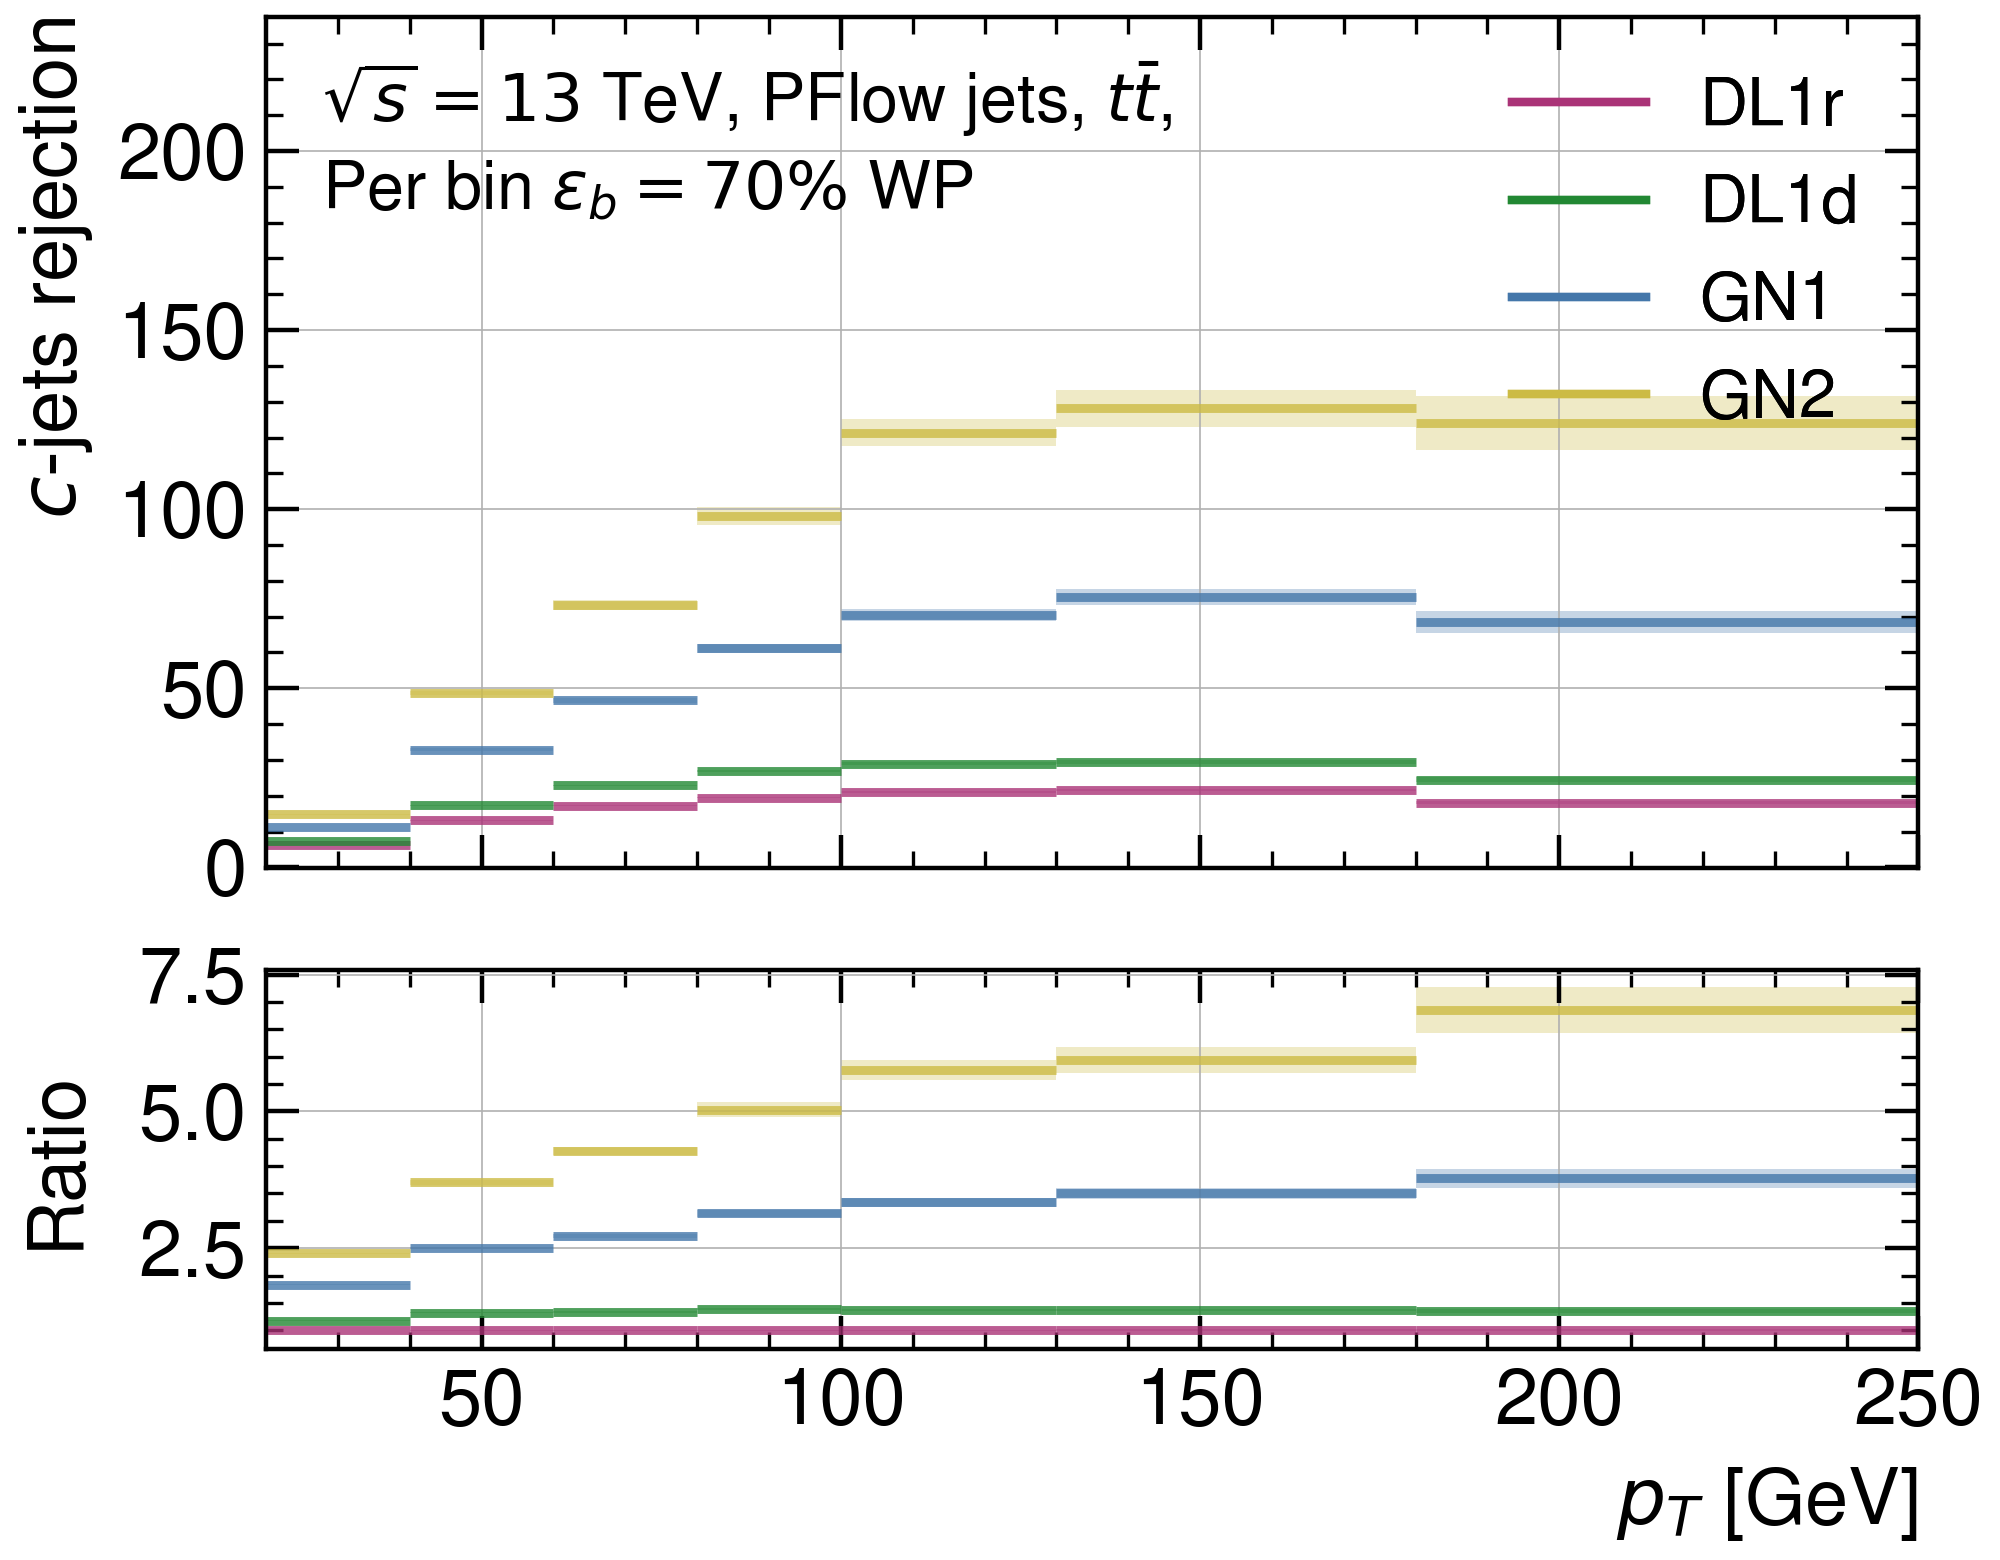
\includegraphics[width=0.48\textwidth]{Images/FTAG/GN/GN2/pt_plots/pt_ttbar_flat_c_rej.png}
  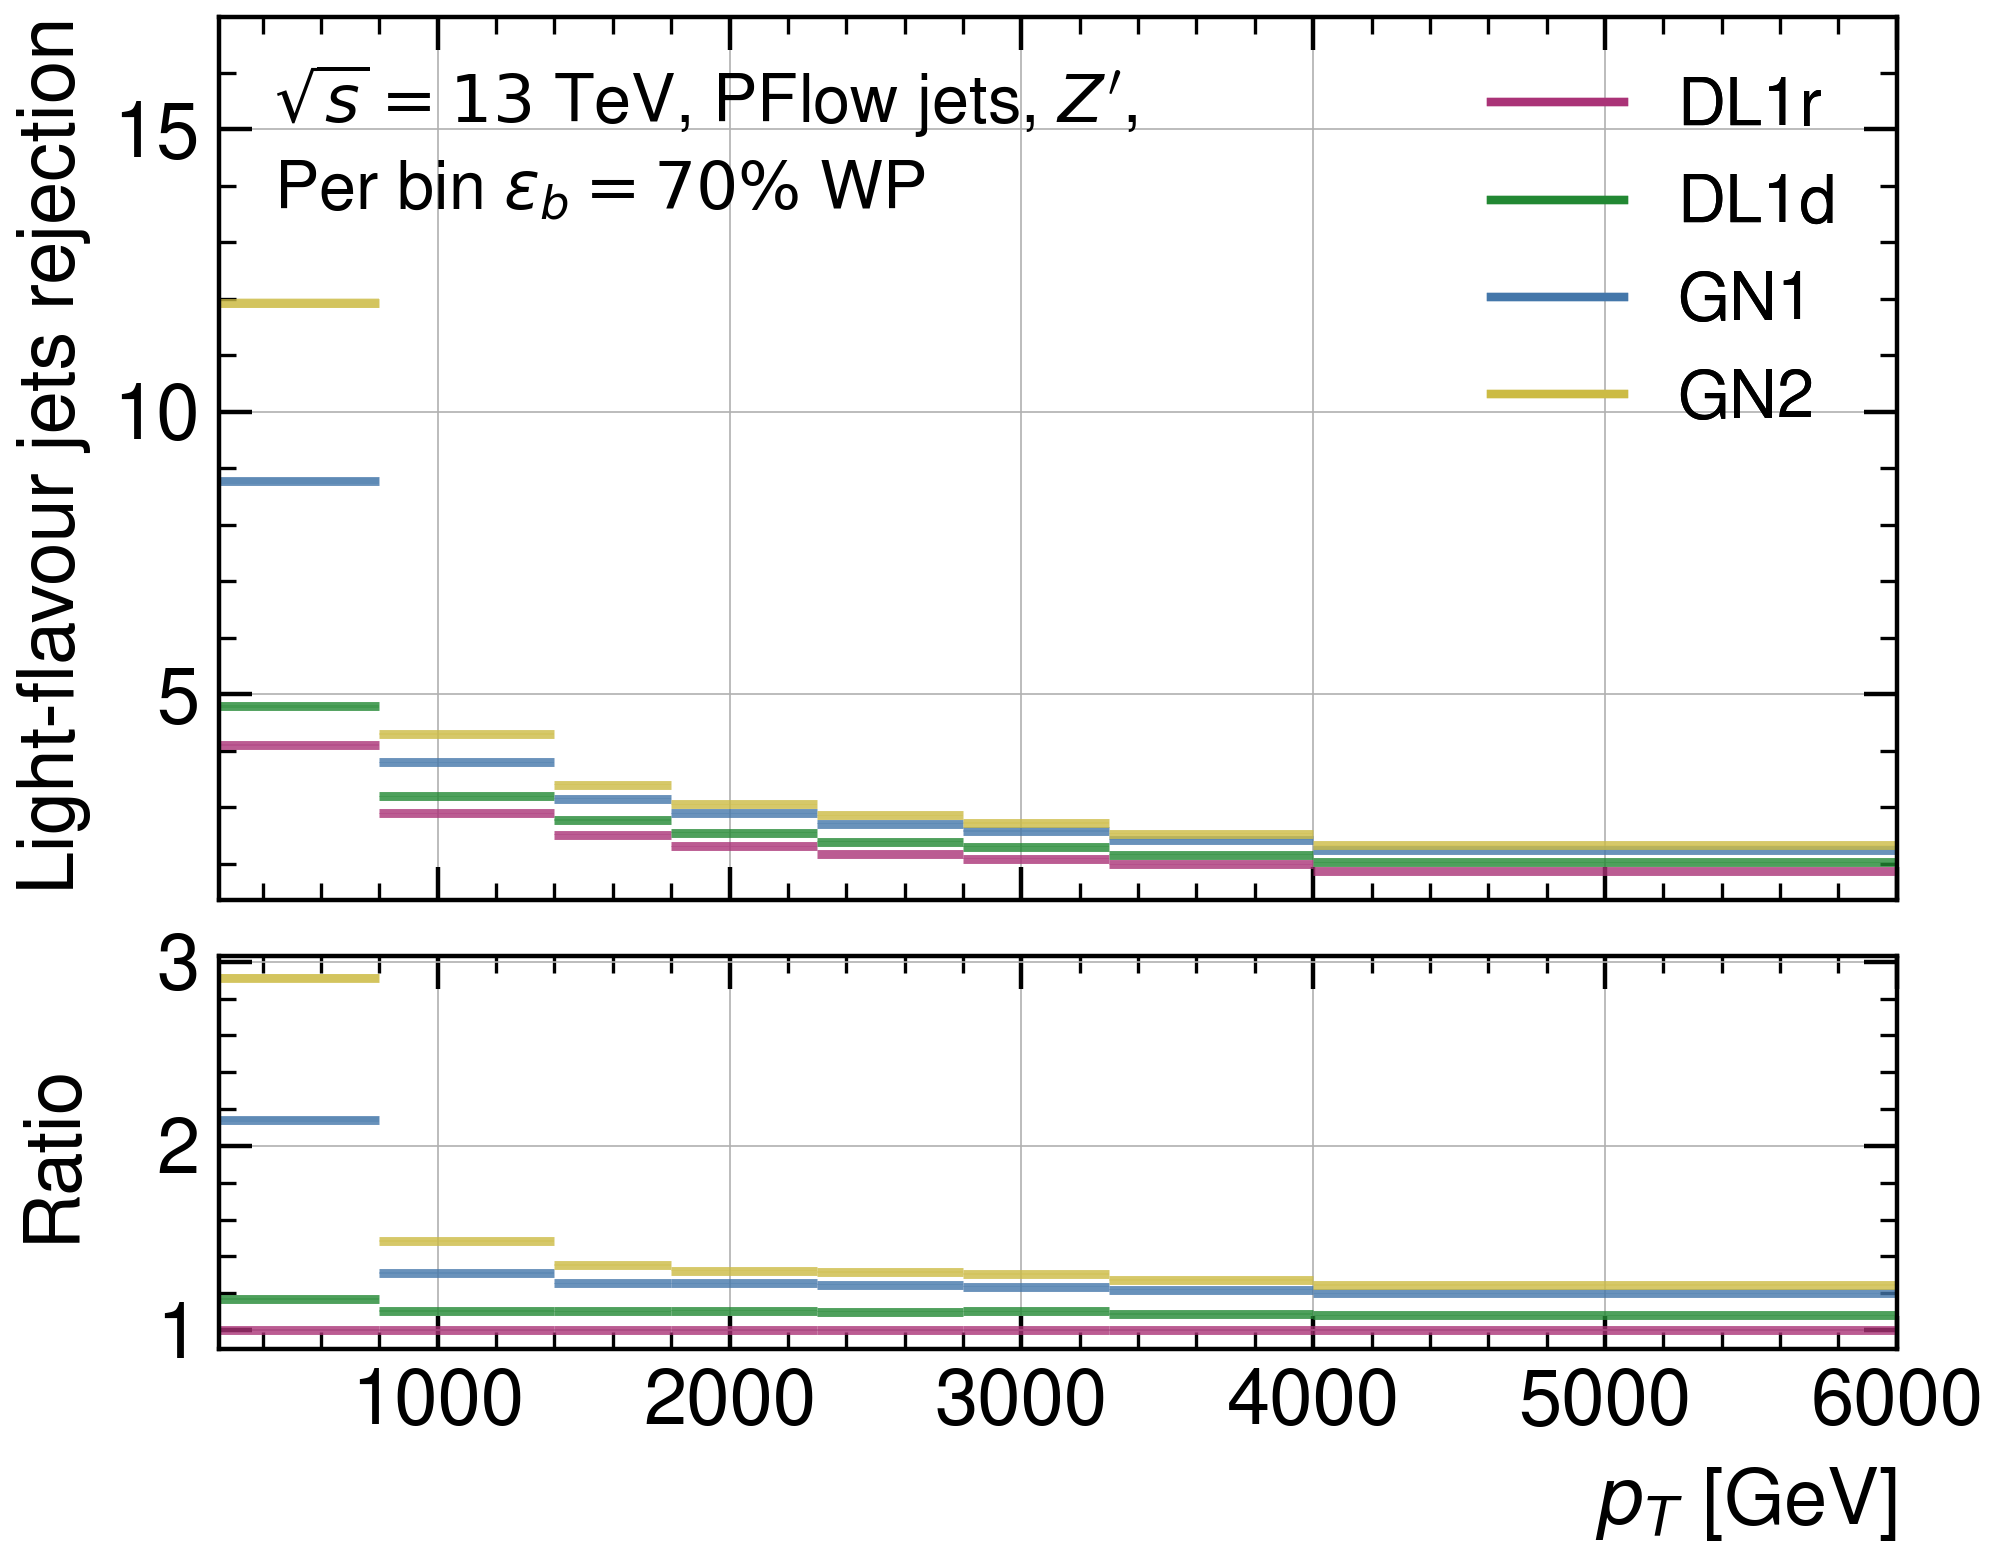
\includegraphics[width=0.48\textwidth]{Images/FTAG/GN/GN2/pt_plots/pt_zp_flat_c_rej.png}
  \caption{Comparing the different models $c$-rejection as a function of jet $p_T$ for the $b$-tagging 70\% \gls{wp} per bin on the $t\bar{t}$ (left) and the 30\% \gls{wp} per bin on $Z'$ (right). The flavour fraction is set at $f^b_c = 0.018$ for DL1r and DL1d, 0.05 for GN1, and 0.1 for GN2.}
  \label{fig:GNxptb_crejflat}
\end{figure} 

% Rej light -flat  btagging
\begin{figure}[h!]
  \centering
  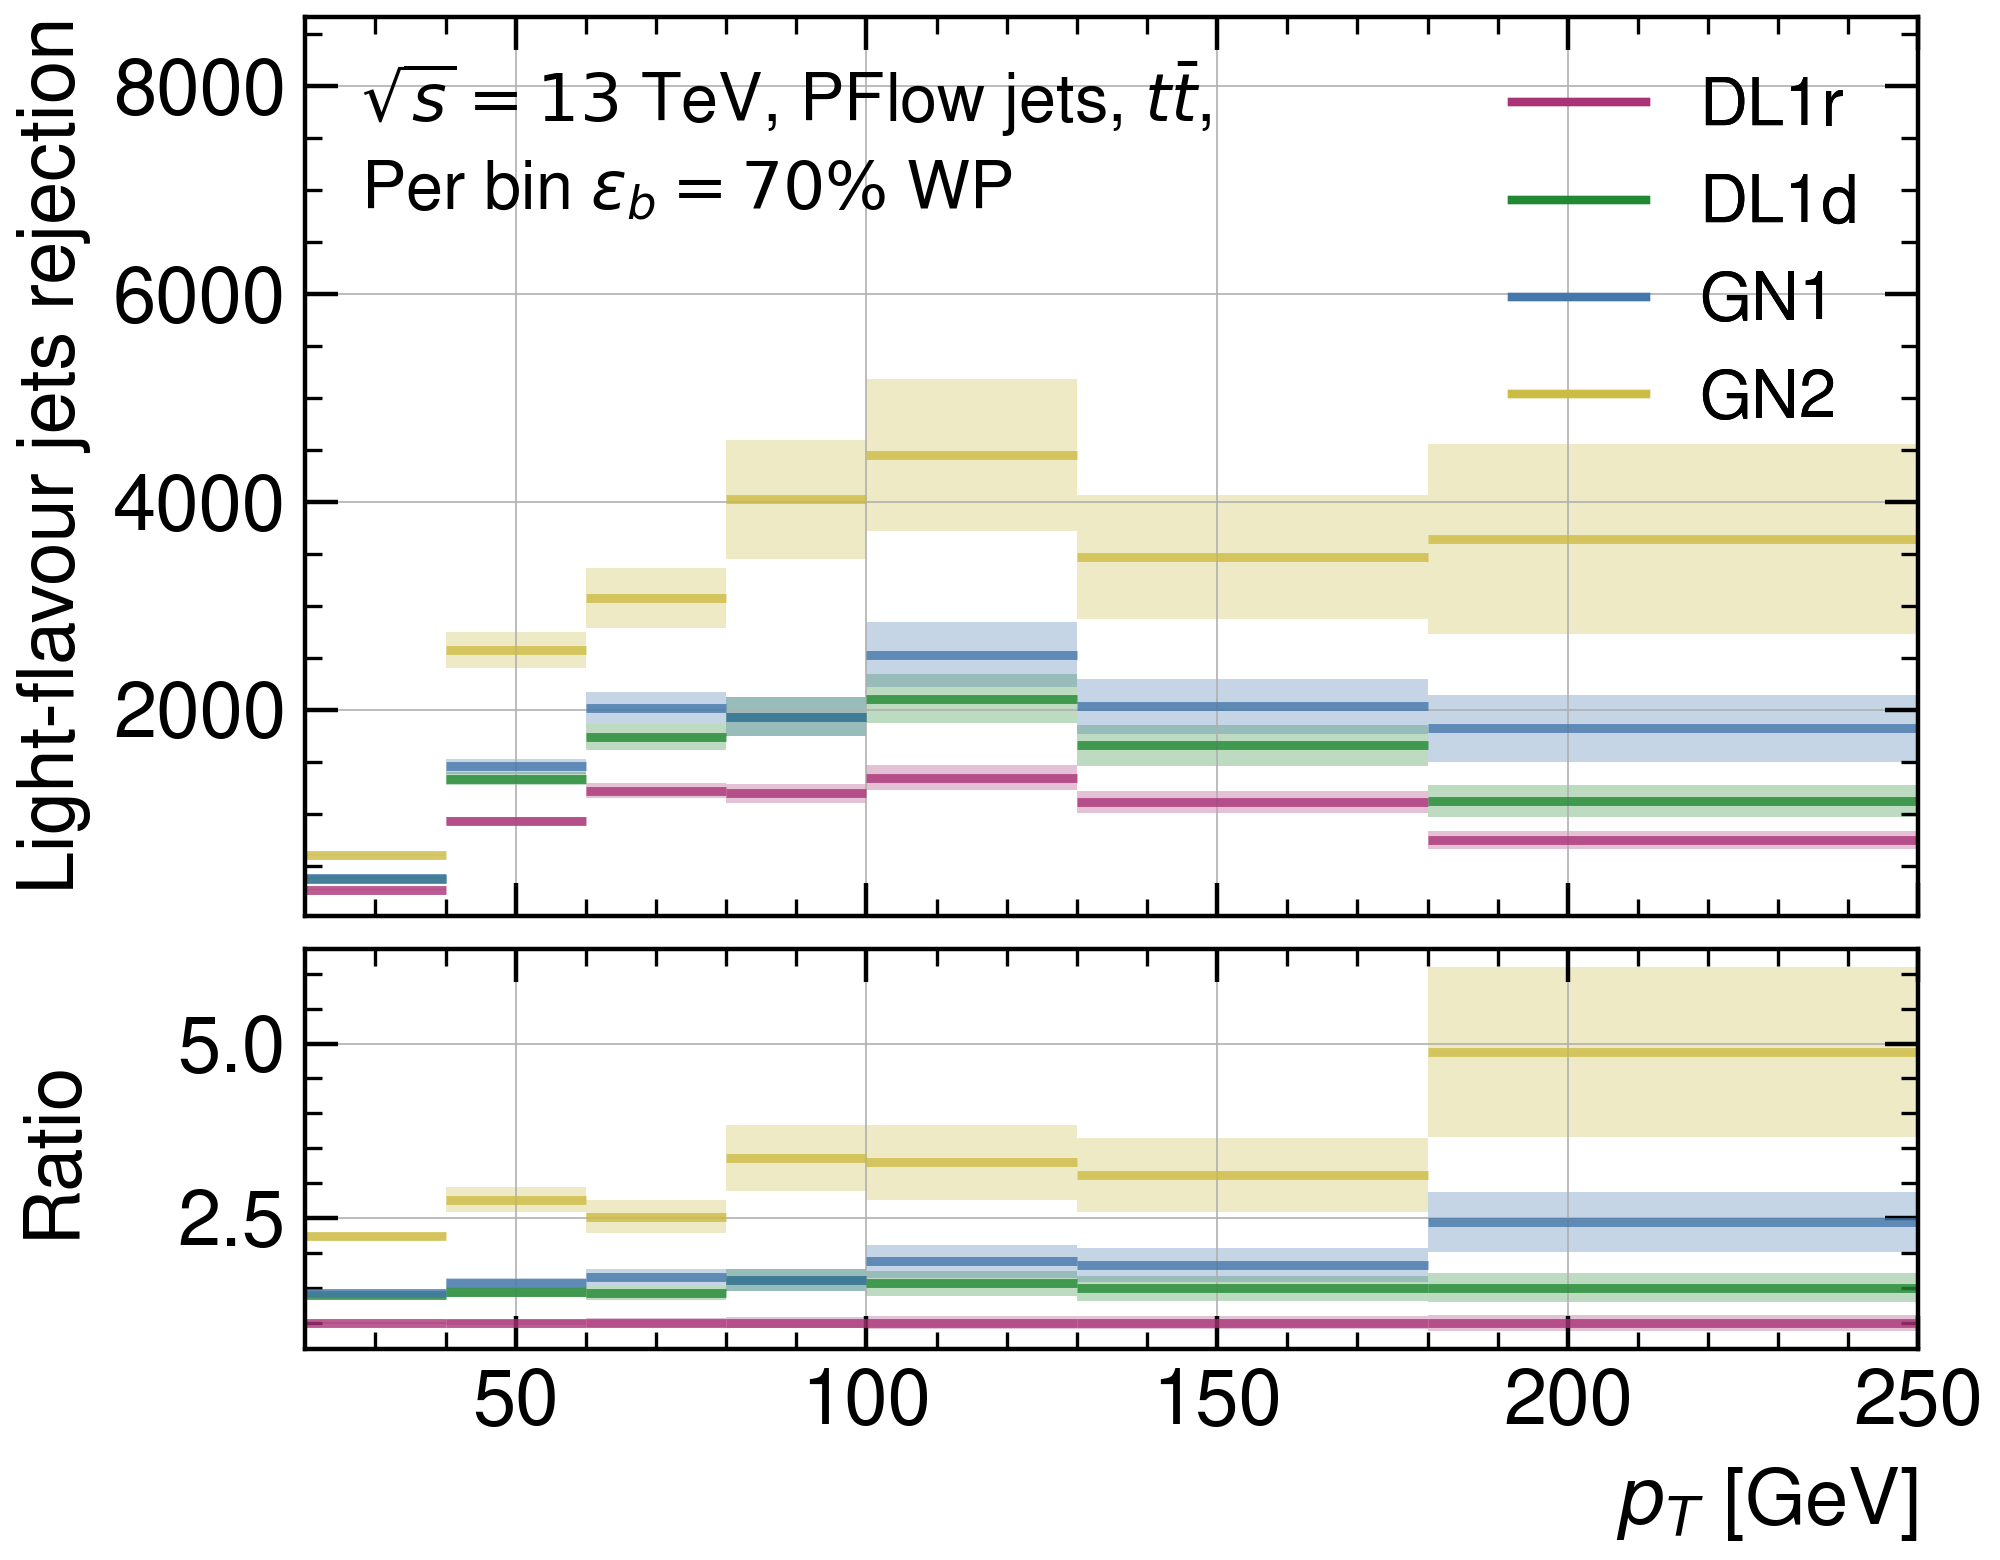
\includegraphics[width=0.48\textwidth]{Images/FTAG/GN/GN2/pt_plots/pt_ttbar_flat_light_rej.png}
  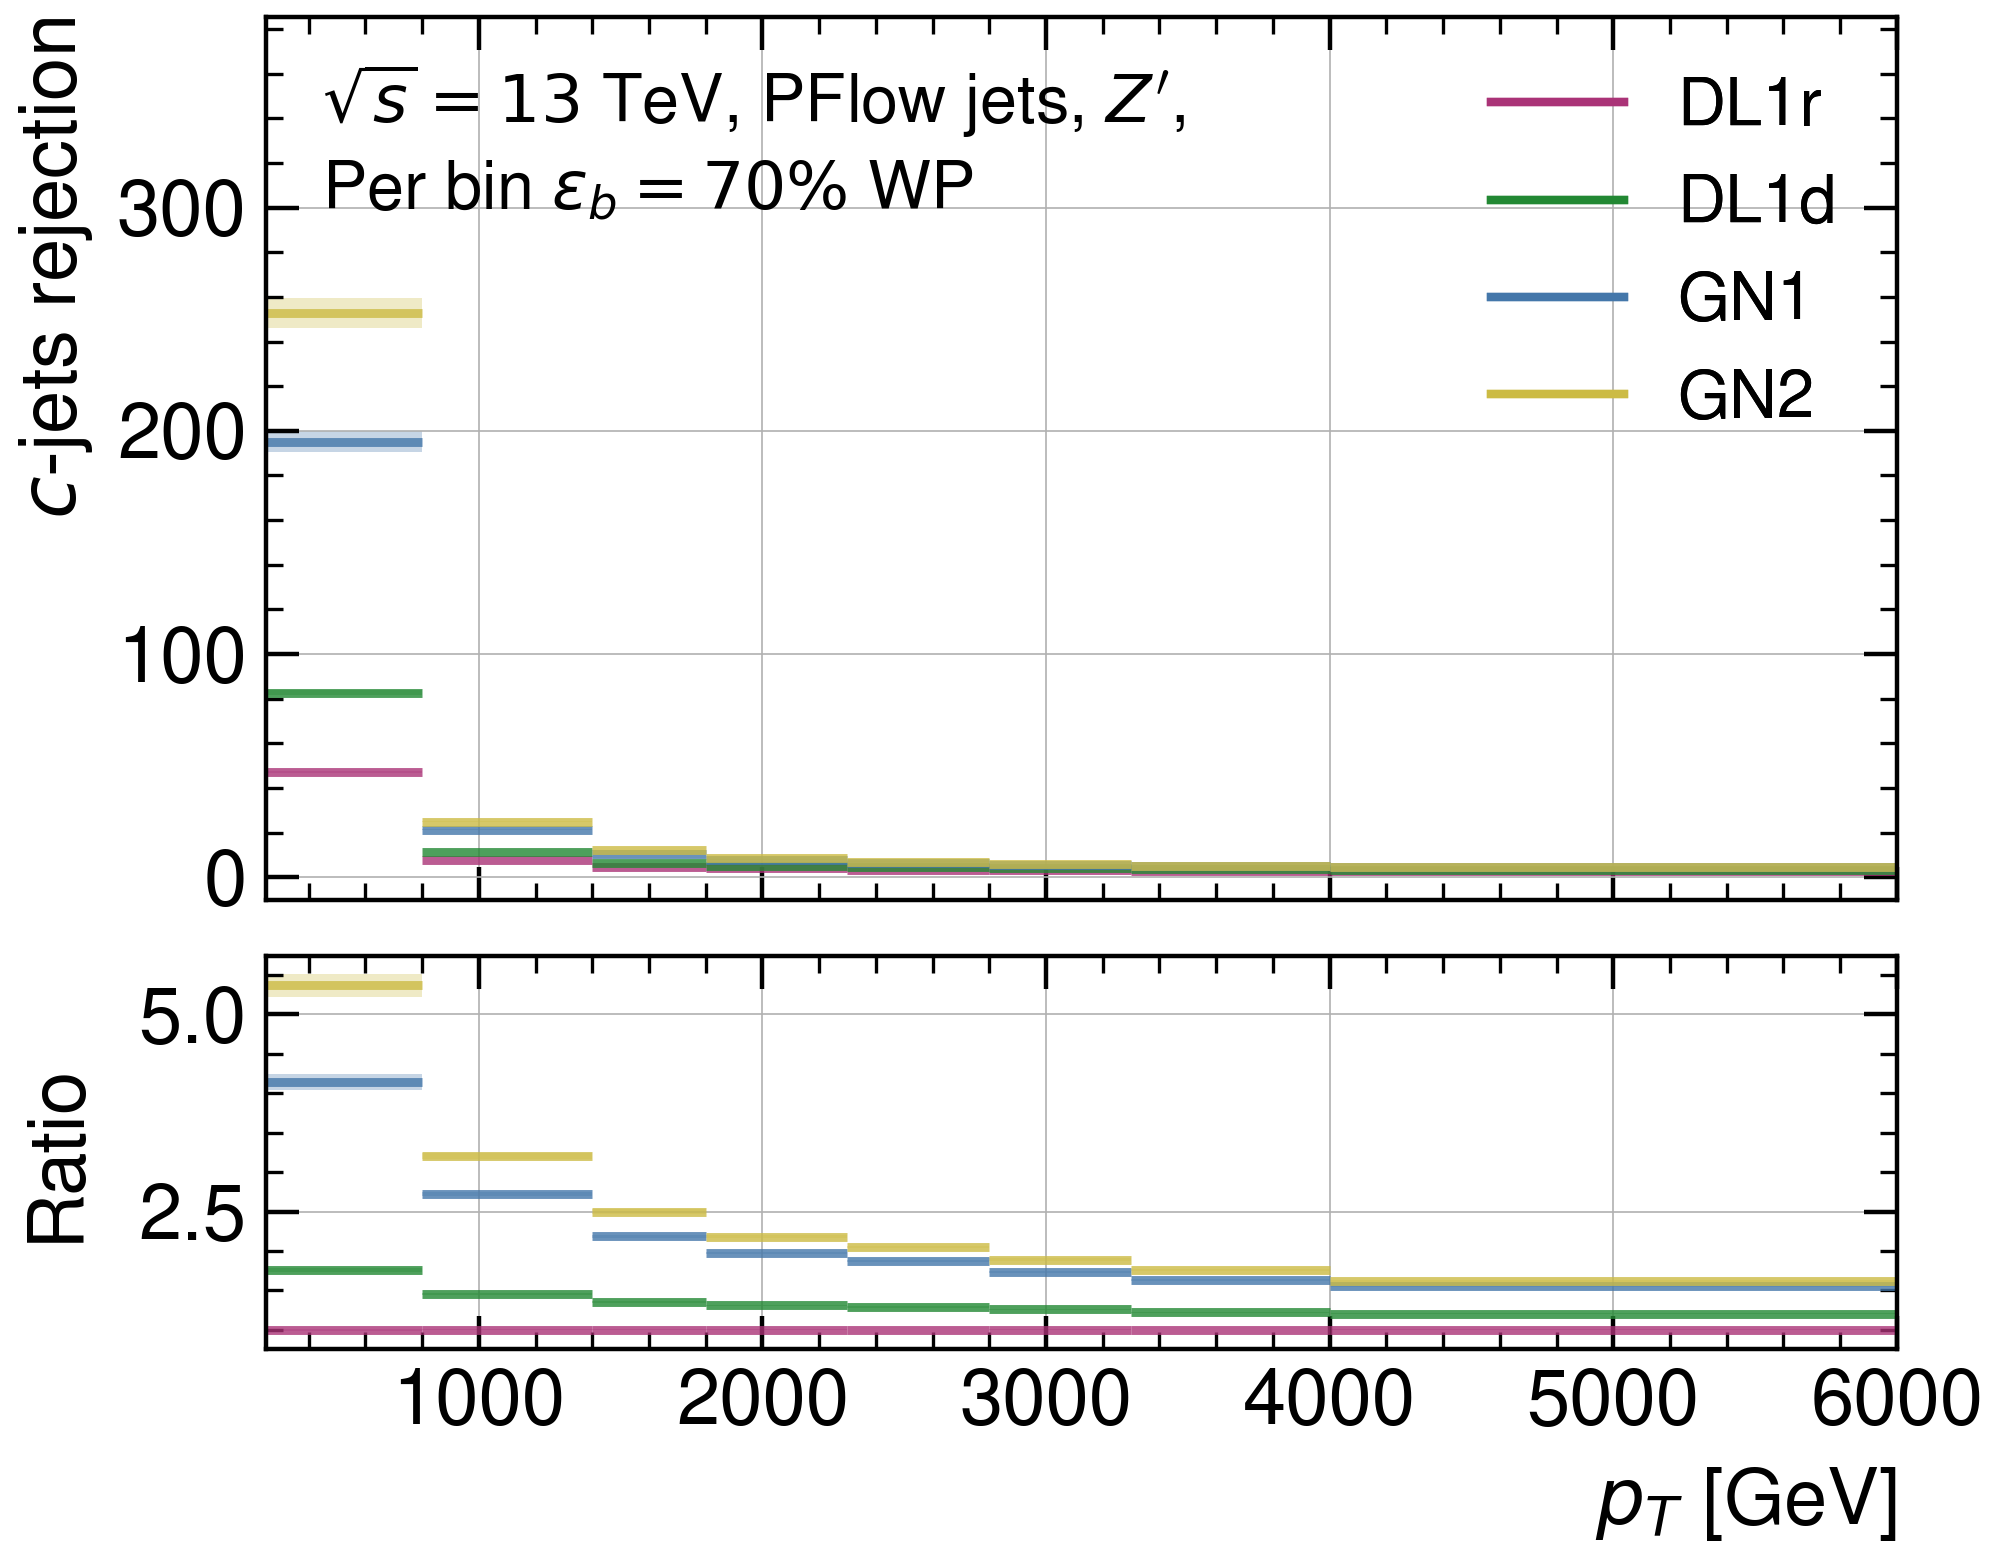
\includegraphics[width=0.48\textwidth]{Images/FTAG/GN/GN2/pt_plots/pt_zp_flat_light_rej.png}
  \caption{Comparing the different models light-rejection as a function of jet $p_T$ for the $b$-tagging 70\% \gls{wp} per bin on the $t\bar{t}$ (left) and the 30\% \gls{wp} per bin on $Z'$ (right). The flavour fraction is set at $f^b_c = 0.018$ for DL1r and DL1d, 0.05 for GN1, and 0.1 for GN2.}
  \label{fig:GNxptb_urejflat}
\end{figure} 

%%%

% Rej b - flat ctagging
\begin{figure}[h!]
  \centering
  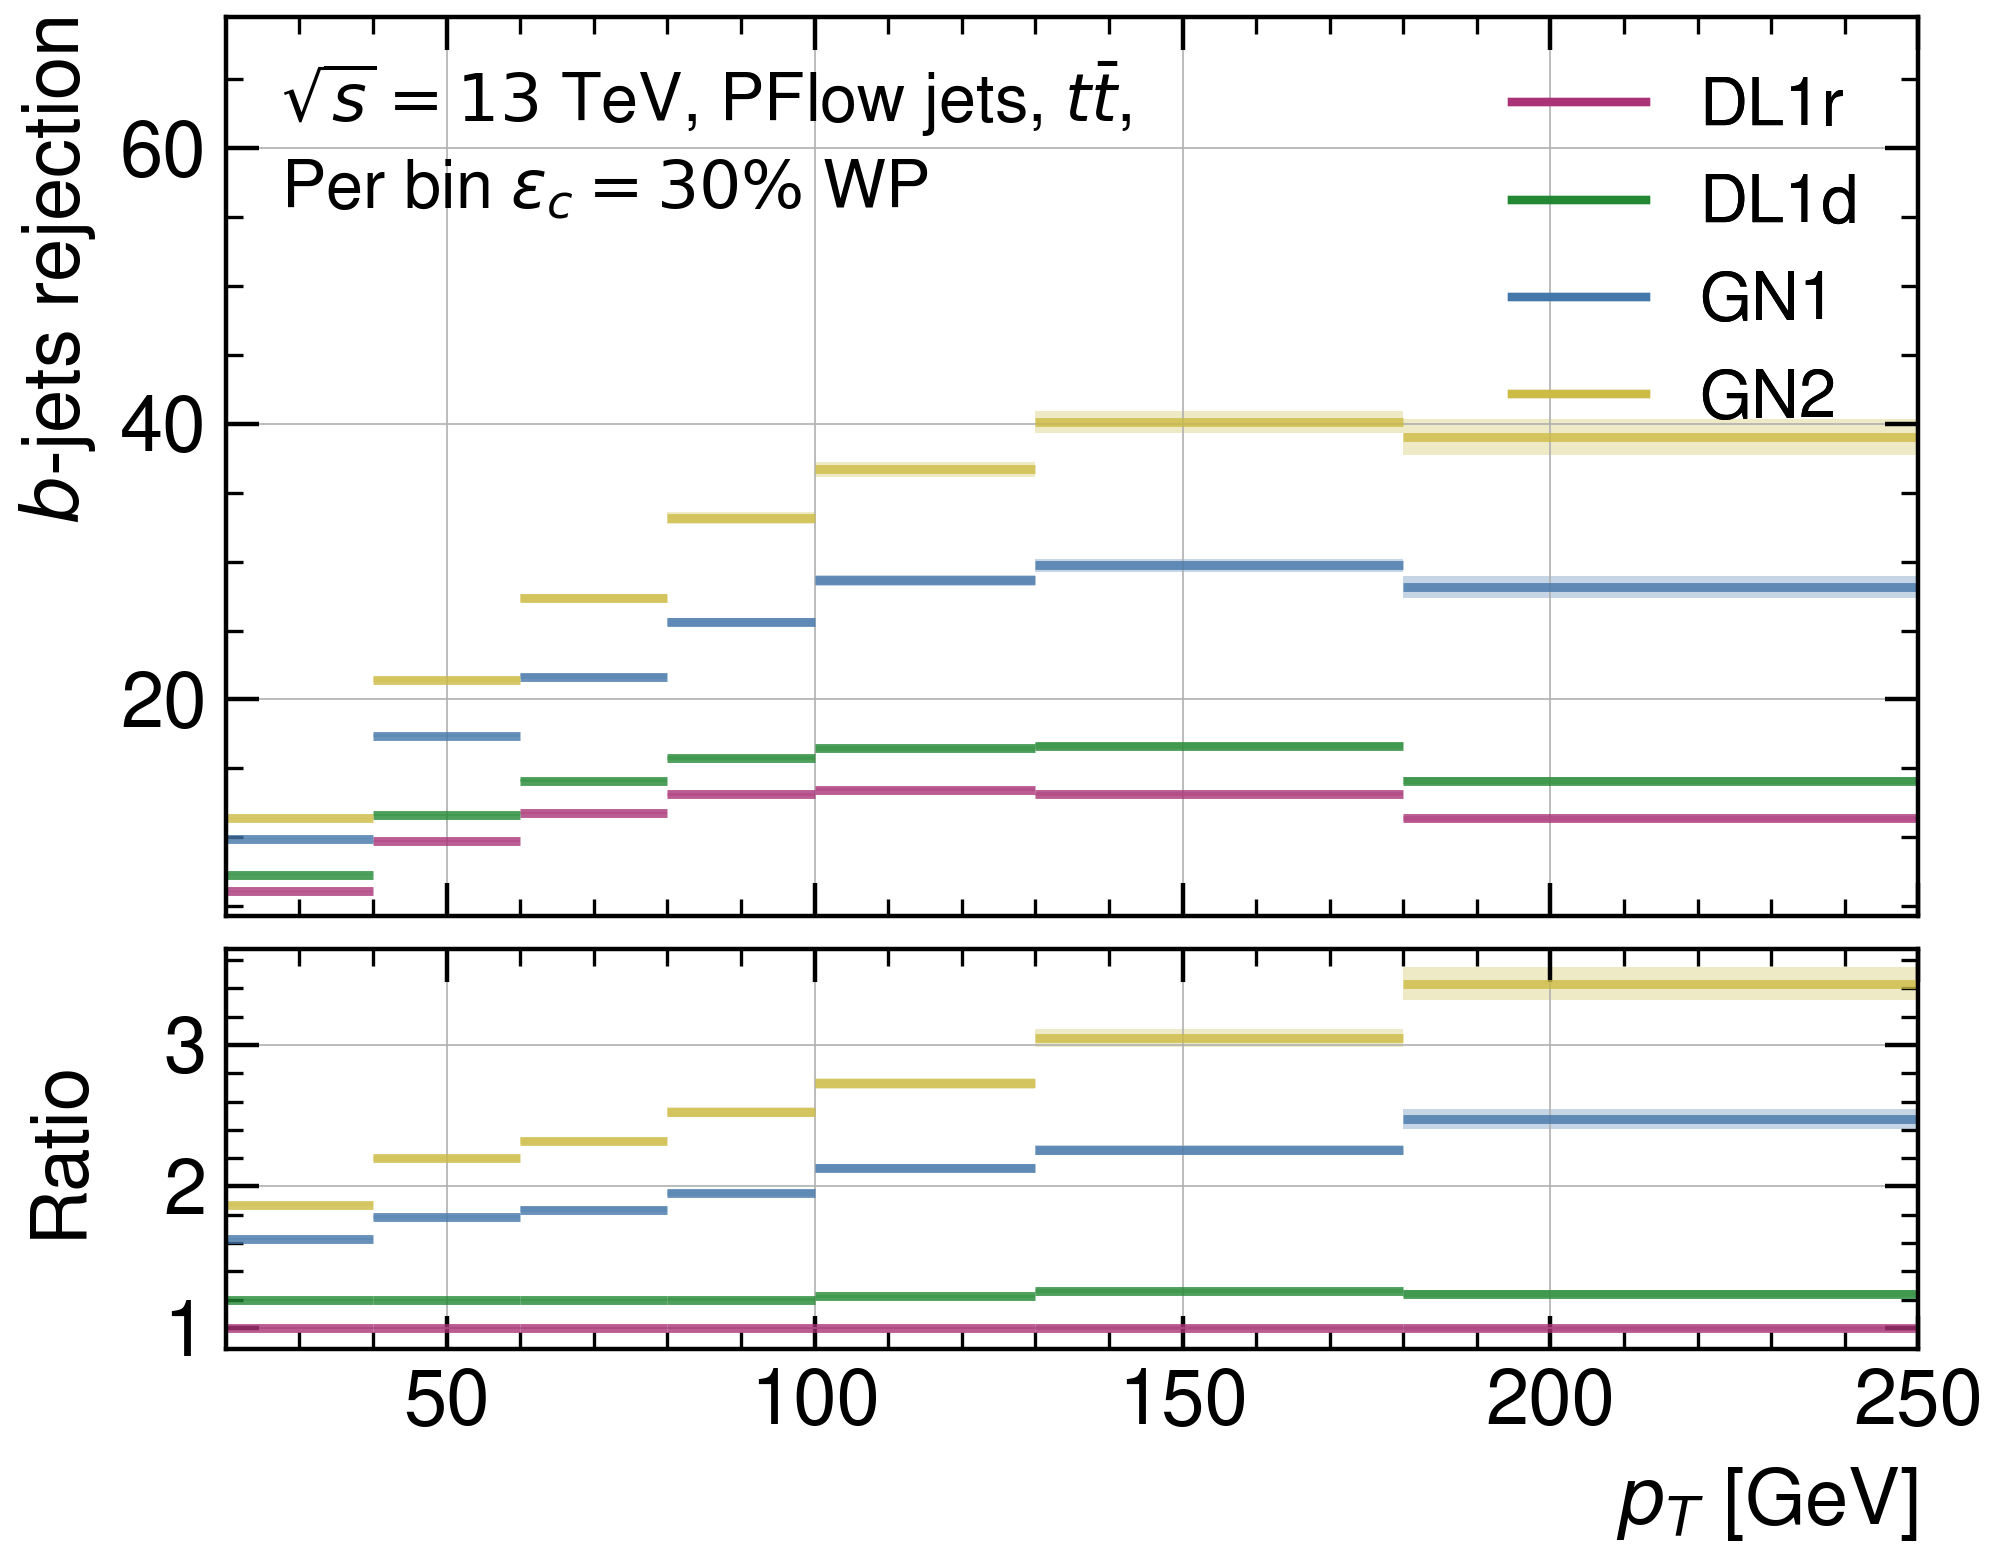
\includegraphics[width=0.48\textwidth]{Images/FTAG/GN/GN2/pt_plots/pt_ttbar_flat_b_rej_c.png}
  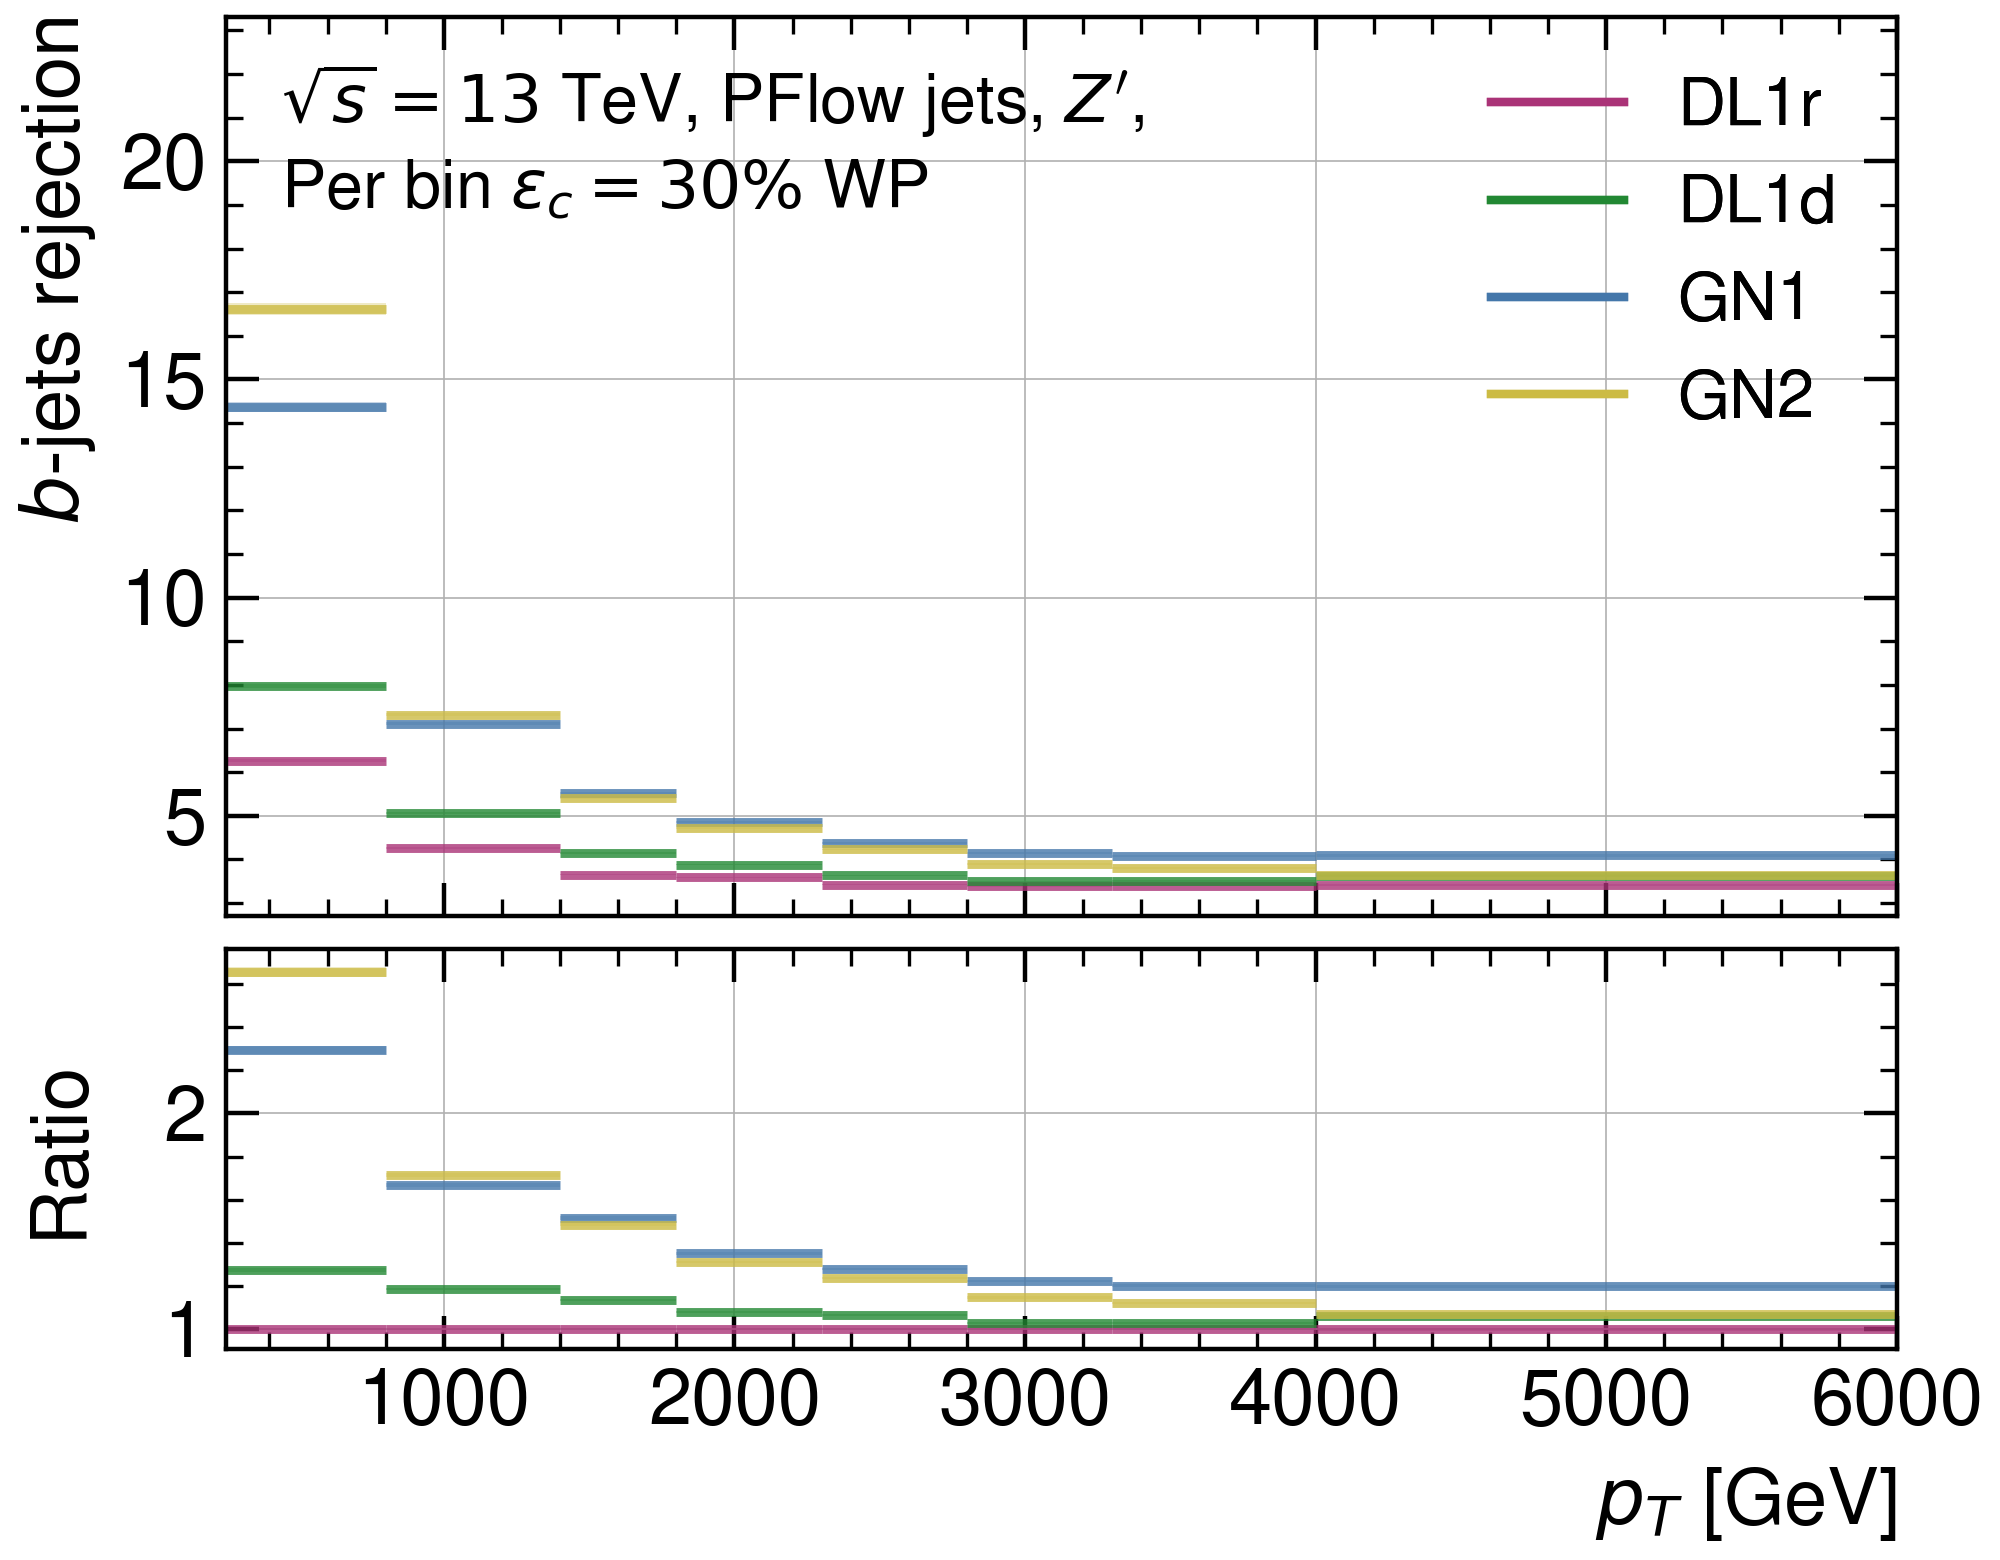
\includegraphics[width=0.48\textwidth]{Images/FTAG/GN/GN2/pt_plots/pt_zp_flat_b_rej_c.png}
  \caption{Comparing the different models $b$-rejection as a function of jet $p_T$ for the $c$-tagging 30\% \gls{wp} per bin on the $t\bar{t}$ (left) and $Z'$ (right). The flavour fraction is set at $f^c_b = 0.2$ for all taggers.}
  \label{fig:GNxptc_brejflat}
\end{figure} 

% Rej light -flat  ctagging
\begin{figure}[h!]
  \centering
  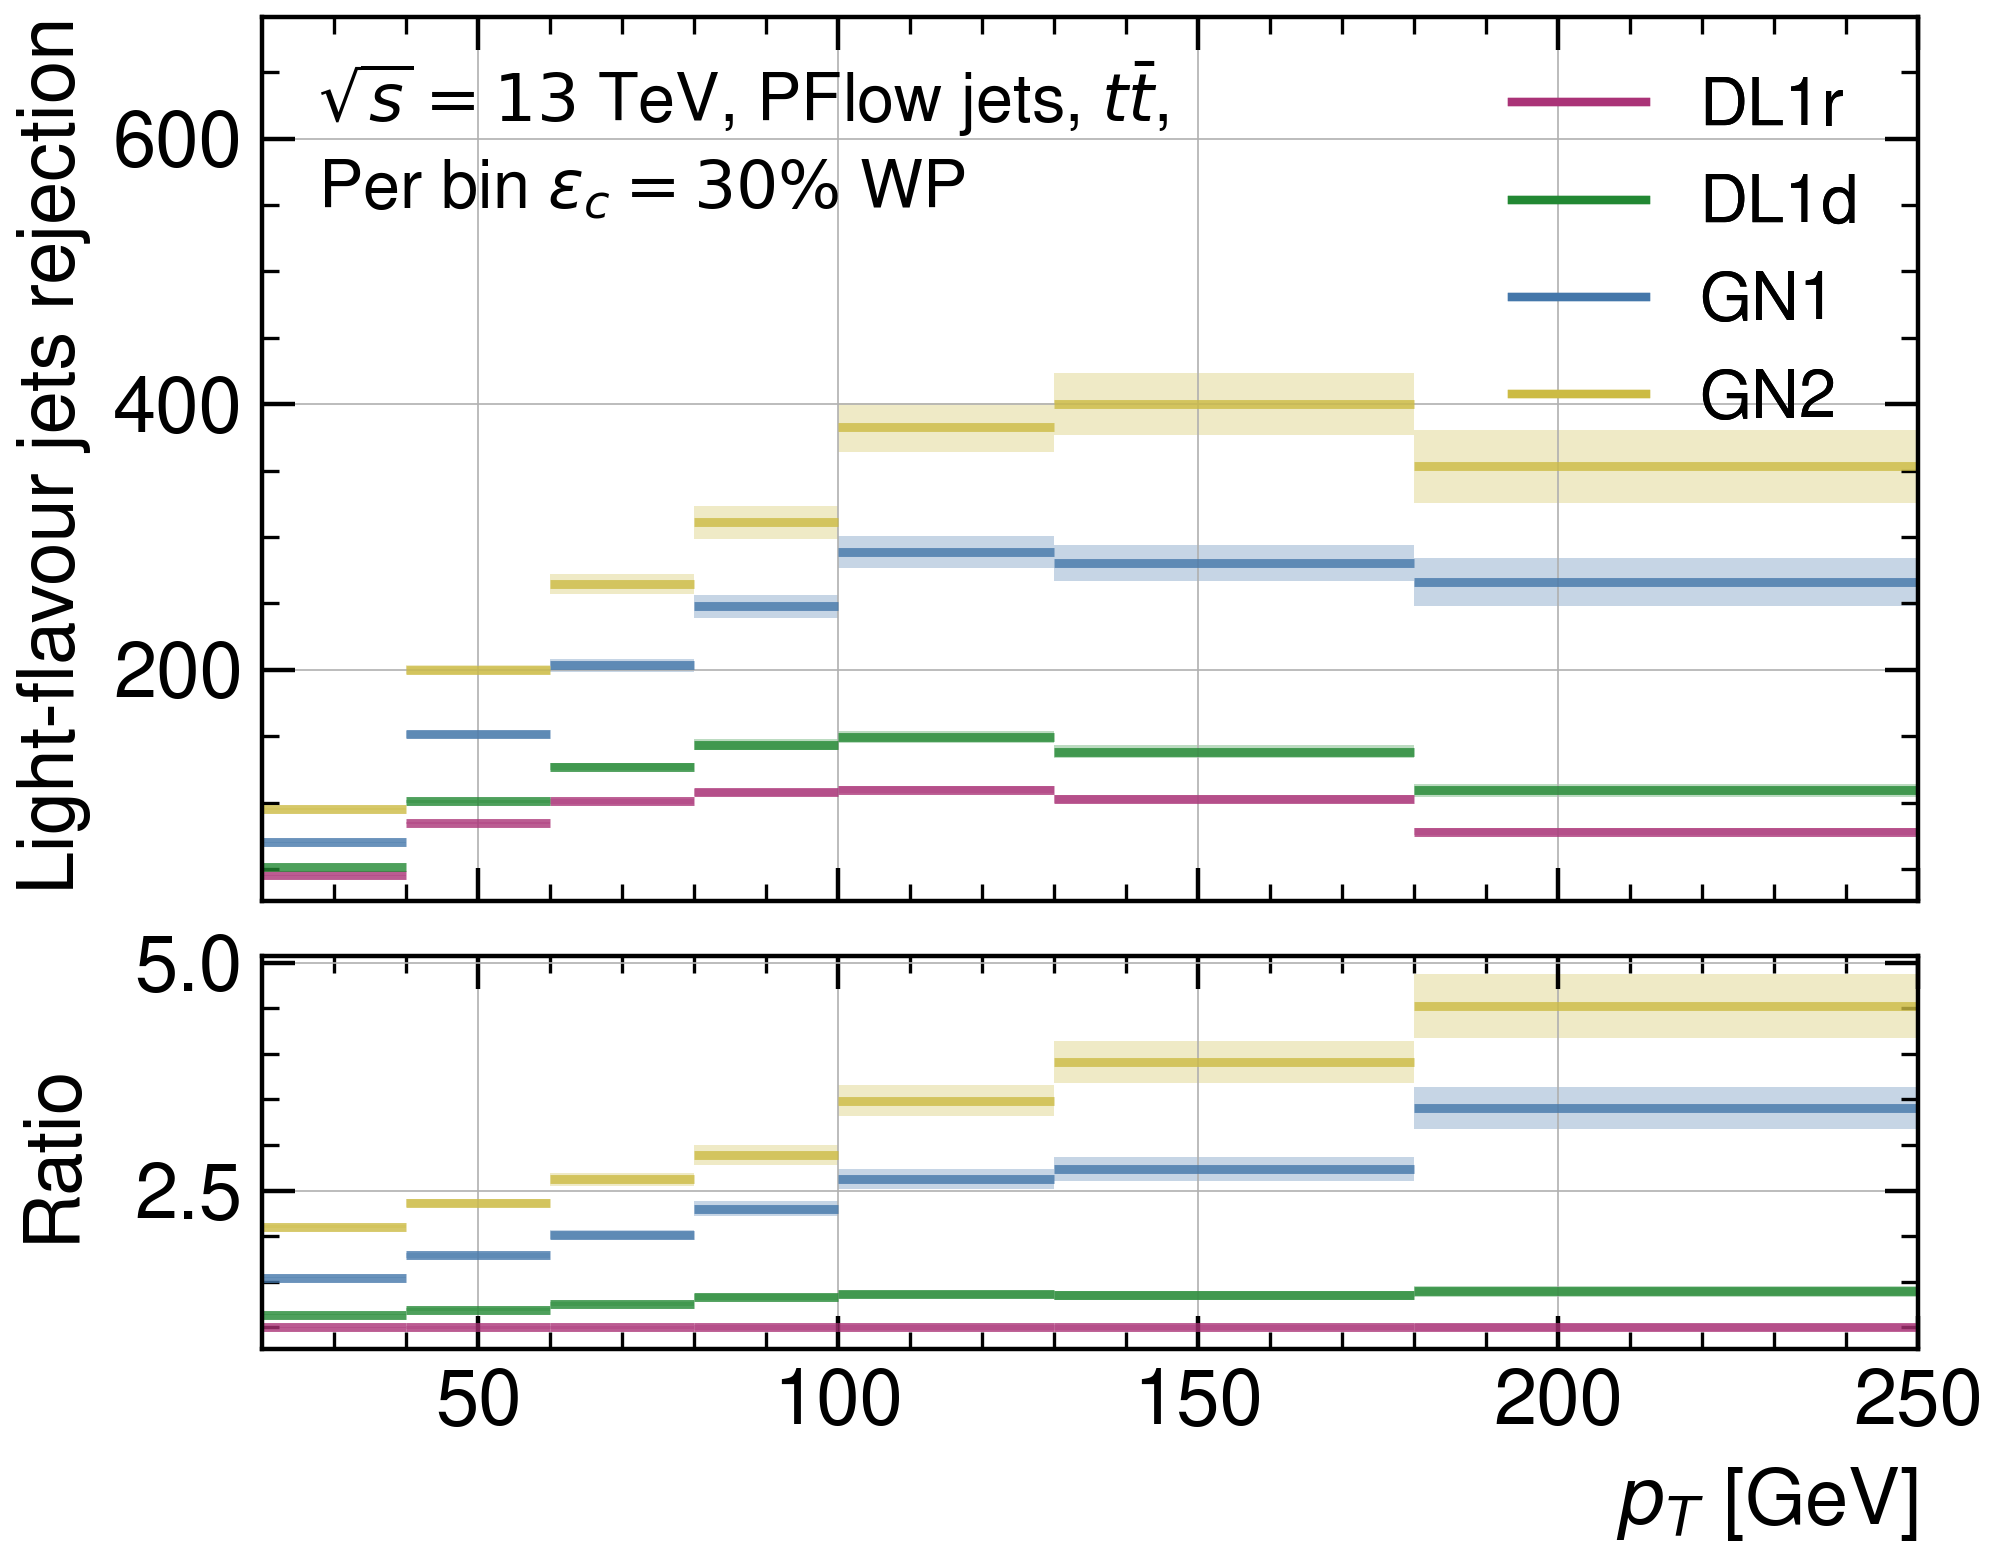
\includegraphics[width=0.48\textwidth]{Images/FTAG/GN/GN2/pt_plots/pt_ttbar_flat_light_rej_c.png}
  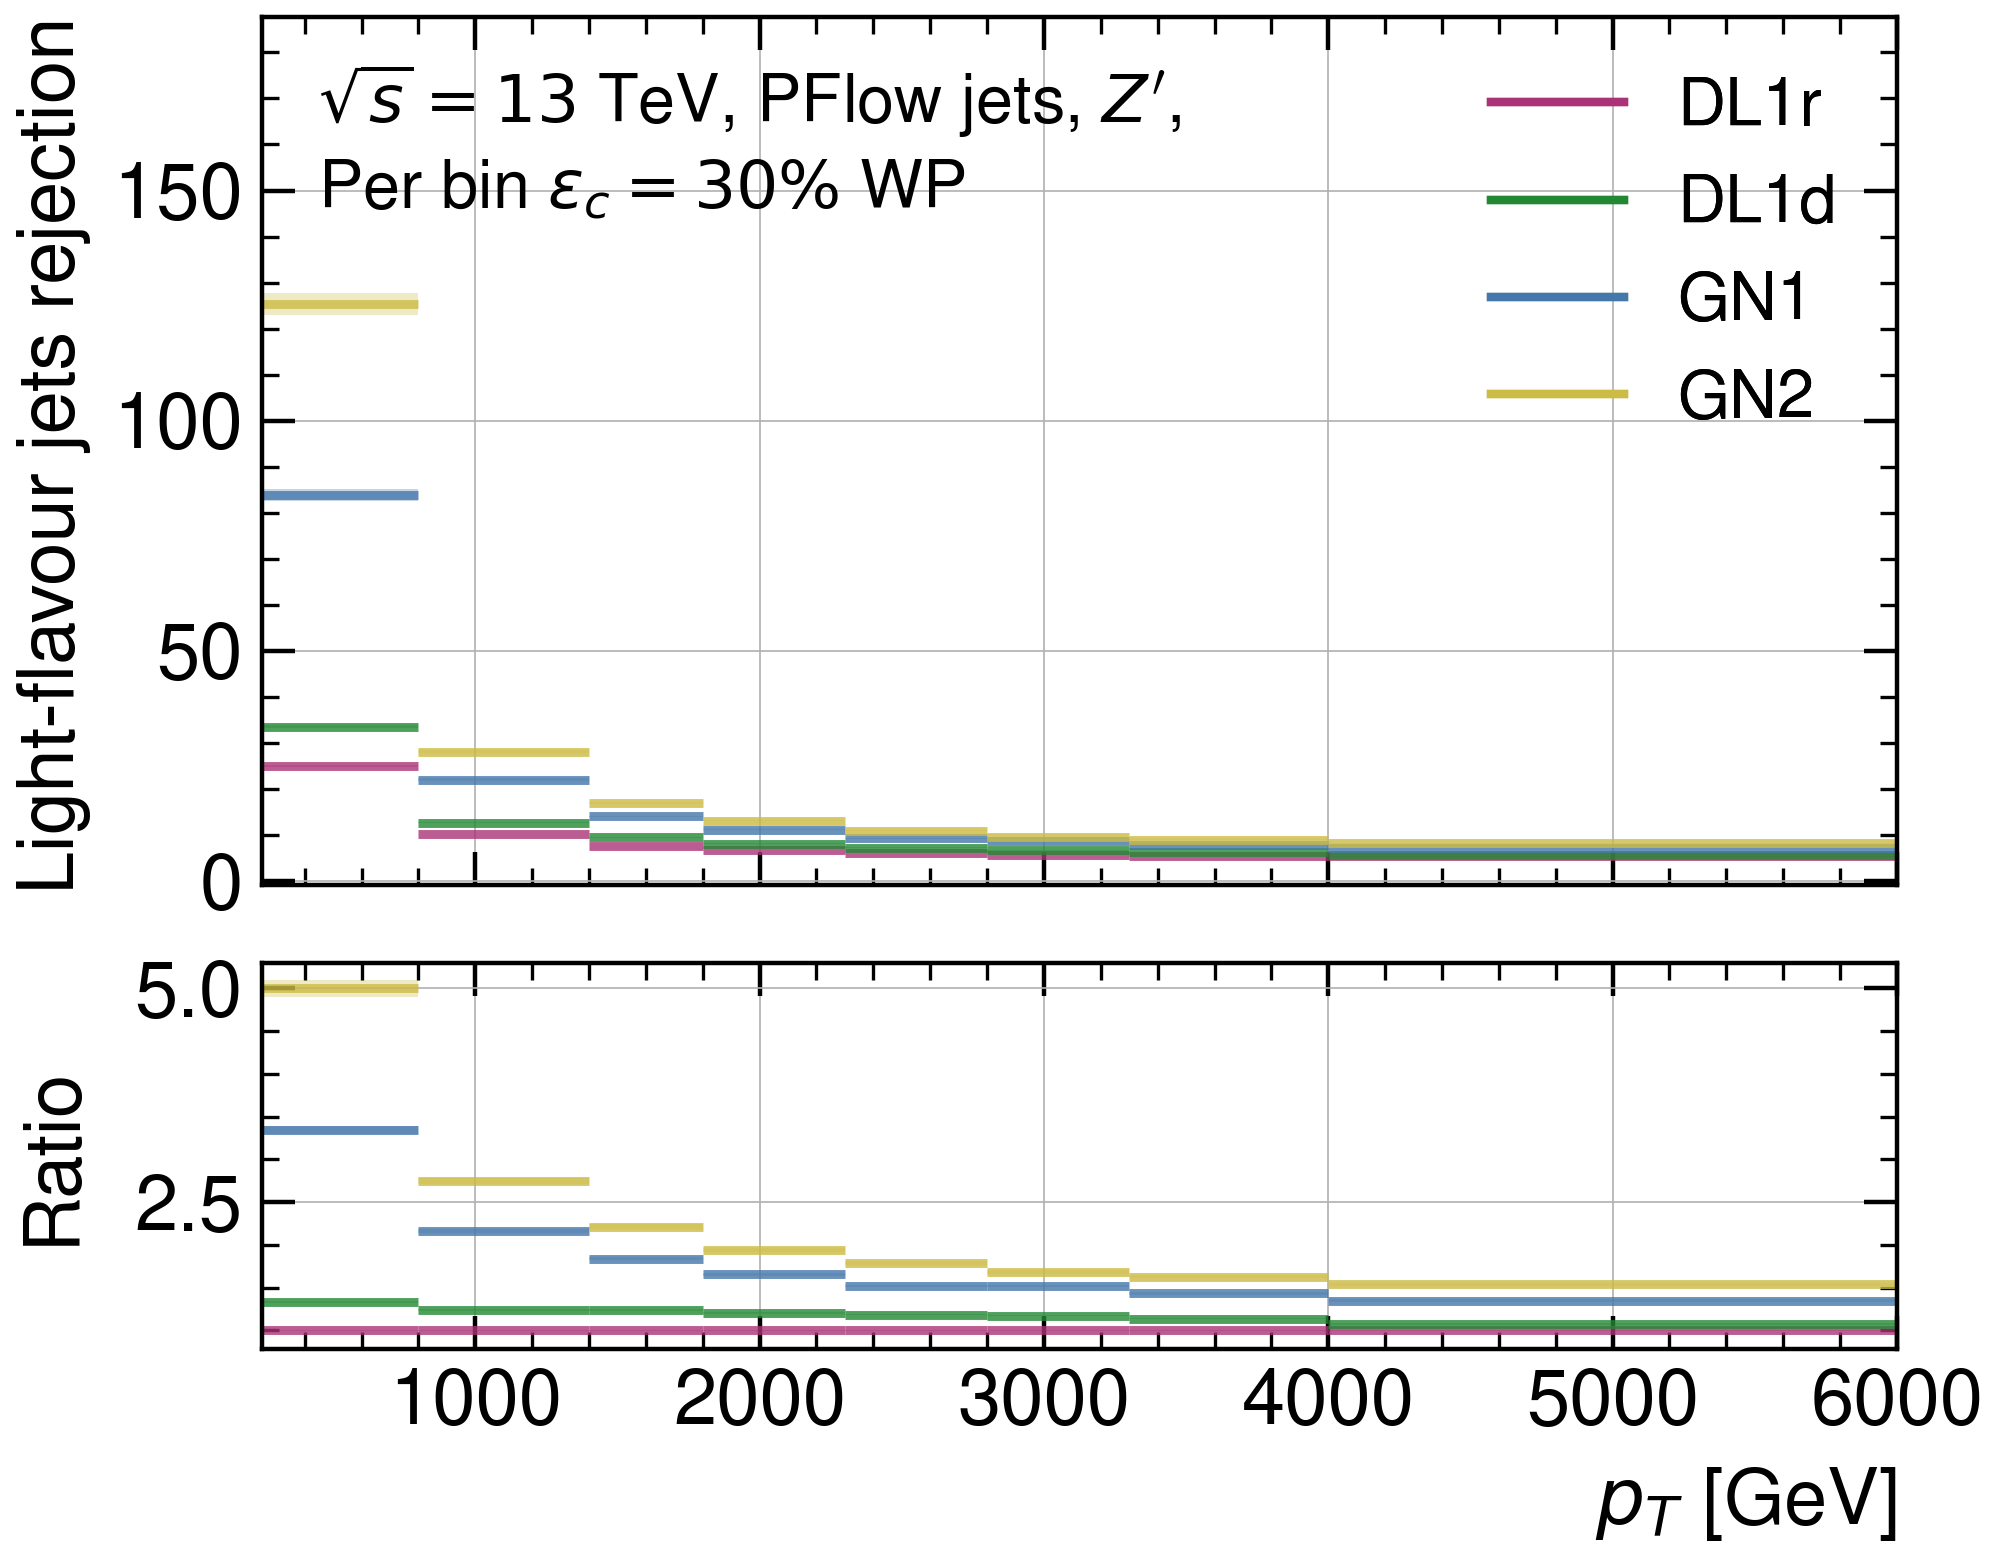
\includegraphics[width=0.48\textwidth]{Images/FTAG/GN/GN2/pt_plots/pt_zp_flat_light_rej_c.png}
  \caption{Comparing the different models light-rejection as a function of jet $p_T$ for the $c$-tagging 30\% \gls{wp} per bin on the $t\bar{t}$ (left) and $Z'$ (right). The flavour fraction is set at $f^c_b = 0.2$ for all taggers.}
  \label{fig:GNxptc_urejflat}
\end{figure} 

These results, albeit intermediary as the development of the new tagger is still underway at the time of writing, are highly suggestive of the promised performance unleashed by the now ATLAS state-of-the-art \gls{gn2} model. Leveraging a simpler design and a more parallelisable architecture, \gls{gn2} can effectively grow to a larger amount of parameters and process larger datasets with no significant overtraining occurring. \gls{rnnip} and \gls{dips} required 50-60k parameters which, once introduced in the high-level algorithm to form \gls{dl1r} and \gls{dl1d}, give rise to models with $\sim$130k parameters. \gls{gn1} revolutionises the approach by adopting a single powerful architecture with a total of $\sim$800k parameters. \gls{gn2} modifies this radical new design to adopt a highly efficient, regularised, and parallelisable model that easily scales the number of parameters to $\sim$1200k, being the first flavour tagger to cross the 1 million parameters threshold. The latest design of \gls{gn2} uses 2.6M parameters, and some tests have raised this number to $\sim$70M parameters. Expert knowledge is passed to the latest generation of models using supervised attention, framing the physics intuition as learnable tasks enforced during training instead of as subtechniques that need to be manually optimised and maintained. Thanks to the flexibility of the \textsc{salt} software \cite{SaltCite}, \gls{gn2} has been successfully optimised for boosted object tagging, with the GN2X tagger presented in Appendix~\ref{app-chap-GN2X} \cite{ATL-PHYS-PUB-2023-021}.
